\documentclass[compress]{beamer}

%--------------------------------------------------------------------------
% Common packages
%--------------------------------------------------------------------------
\usepackage[english]{babel}
\usepackage{pgfpages} % required for notes on second screen
\usepackage{graphicx}
\usepackage{subfigure}
\usepackage{multicol}
\usepackage[normalem]{ulem}

\usepackage{tabularx,ragged2e}
\usepackage{booktabs}
\usepackage{marvosym}

%--------------------------------------------------------------------------
% Load theme
%--------------------------------------------------------------------------
\usetheme{hri}

\usepackage{tikz}
\usetikzlibrary{patterns,shapes,fpu,fit,calc,mindmap,backgrounds,positioning,svg.path}

\tikzset{
  invisible/.style={opacity=0},
  visible on/.style={alt={#1{}{invisible}}},
  alt/.code args={<#1>#2#3}{%
    \alt<#1>{\pgfkeysalso{#2}}{\pgfkeysalso{#3}} % \pgfkeysalso doesn't change the path
  },
}

%% Neat trick to have only one navigation bullet per subsection
%% http://tex.stackexchange.com/questions/64333/one-navigation-bullet-per-subsection-with-subsection-false-in-custom-beamer-them
%\usepackage{etoolbox}
%\makeatletter
%\patchcmd{\slideentry}{\advance\beamer@xpos by1\relax}{}{}{}
%\def\beamer@subsectionentry#1#2#3#4#5{\advance\beamer@xpos by1\relax}%
%\makeatother
%%%%%%%%%%%%%%%%%%%%%%%%%%%%%%%%%%%%%%%

\graphicspath{{figs/}}

% for model of anthopomorphism
\newcommand{\IPA}{{$\mathcal{A}_0$~}}
\newcommand{\SLA}{{$\mathcal{A}_\infty$~}}
\newcommand{\sla}{{\mathcal{A}_\infty}}
\newcommand{\AntMax}{{$\mathcal{A}_{max}$~}}
\newcommand{\antMax}{{\mathcal{A}_{max}}}

% for HATP plans
\newcommand{\hatpaction}[3]{#1\\\textsf{\scriptsize #2,}\\\textsf{\scriptsize #3}}
\newcommand{\stmt}[1]{{\footnotesize \tt  #1}}

% for mutual modelling
\newcommand{\Mmodel}[3]{{\mathcal{M}(#1, #2, #3)}}
\newcommand{\model}[3]{{$\mathcal{M}(#1, #2, #3)$}}
\newcommand{\Model}[3]{{$\mathcal{M}^{\circ}(#1, #2, #3)$}}

% typeset logical concept
\newcommand{\concept}[1]{{\scriptsize \texttt{#1}}}

\newcommand{\backbutton}{\hfill\hyperlink{appendix}{\beamerreturnbutton{Supplementary material}}}
%--------------------------------------------------------------------------
% General presentation settings
%--------------------------------------------------------------------------
\title{Of Cognition and Social Robots}
%\subtitle{towards a theory of artificial social cognition}
\subtitle{}
\date{Plymouth University -- {\bf 14 February 2017}}
\author{Séverin Lemaignan}
\institute{Centre for Robotics and Neural Systems\\{\bf
Plymouth University}}

%--------------------------------------------------------------------------
% Notes settings
%--------------------------------------------------------------------------
%\setbeameroption{show notes on second screen}
%\setbeameroption{hide notes}

\begin{document}


%%%%%%%%%%%%%%%%%%%%%%%%%%%%%%%%%%%%%%%%%%%%%%%%%%%%%%%%


%%%%%%%%%%%%%%%%%%%%%%%%%%%%%%%%%%%%%%%%%%%%%%%%%%%%%%%%

\maketitle

%%%%%%%%%%%%%%%%%%%%%%%%%%%%%%%%%%%%%%%%%%%%%%%%%%%%%%%%

\section*{Curriculum \& Teaching}

\imageframe{europe_map}

\begin{frame}{Academic Curriculum overview}
    \begin{itemize}
        \item<1-> Joint French (ParisTech) German (Karlsruhe Institute of Technology) MSc
            in mechanical engineering
            \begin{itemize}
                \item \textbf{top ten student} out of 1000
            \end{itemize}
        \item<1-> MSc in AI for Learning technologies (University Paris 5)
            \begin{itemize}
                \item \textbf{top student} of the year
            \end{itemize}
        \item<2-> Joint French (CNRS LAAS) German (Technical University of Munich)
            PhD in AI \& Cognitive Robotics
            \begin{itemize}
                \item \textbf{Best 2012 CNRS PhD in Robotics}
                \item \textbf{High Distinction} in Germany
            \end{itemize}

    \end{itemize}

    \onslide<3->

    \vspace{2em}
    To date,\\
    
    \large
    \textbf{50+ publications}; \textbf{920+ citations}; \textbf{H-index=15}

\end{frame}

\begin{frame}{Academic Curriculum overview}
    2013-2015: \textbf{post-doc at EPFL}
    \begin{itemize}
        \item<+-> built up a leading group in child-robot interaction
        \item<+-> from 1 PhD to 3 PhD + 2-3 MSc students
        \item<+-> joint supervisions with Portugal, France
        \item<+-> 2 high-visibility projects with large media coverage
        \item<+-> 7 papers in 4 years at high-profile HRI conference, \textbf{2 awards}
    \end{itemize}

    \onslide<6->
    2015: \textbf{EU Marie Skłodowska-Curie fellow} at Plymouth University on
    \textbf{social cognition for robots}

\end{frame}

\imageframe[color=black]{teaching}

\begin{frame}[plain]

        \begin{center}

            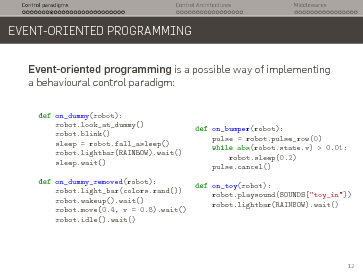
\includegraphics[width=0.3\linewidth]{teaching/events}\hspace{1em}
            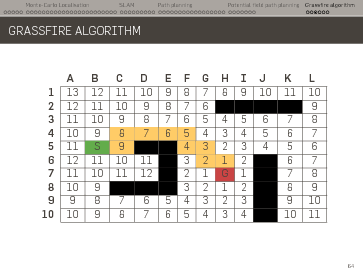
\includegraphics[width=0.3\linewidth]{teaching/grassfire}\hspace{1em}
            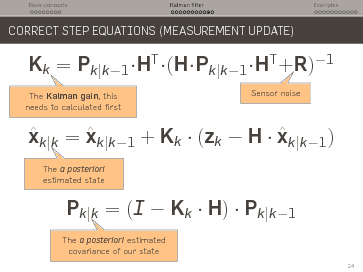
\includegraphics[width=0.3\linewidth]{teaching/kalman}\hspace{1em}

            \pause

            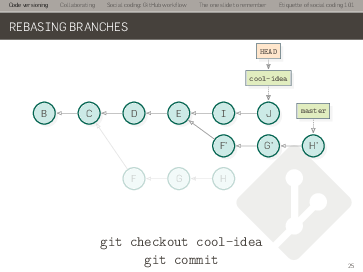
\includegraphics[width=0.3\linewidth]{teaching/git}\hspace{1em}
            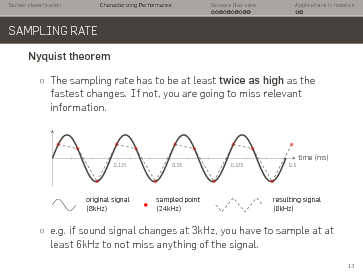
\includegraphics[width=0.3\linewidth]{teaching/nyquist}\hspace{1em}
            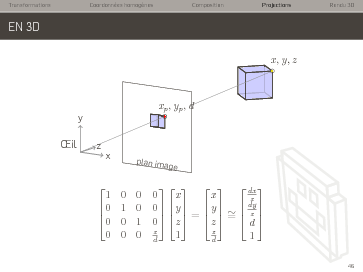
\includegraphics[width=0.3\linewidth]{teaching/3d}\hspace{1em}

            \pause

            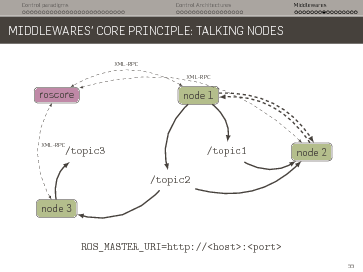
\includegraphics[width=0.3\linewidth]{teaching/ros}\hspace{1em}
            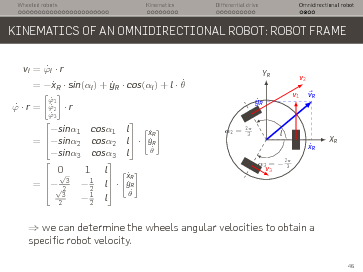
\includegraphics[width=0.3\linewidth]{teaching/omnidirectional}\hspace{1em}
            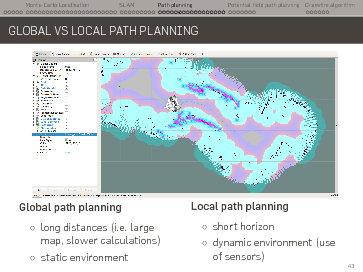
\includegraphics[width=0.3\linewidth]{teaching/costmap}\hspace{1em}

        \end{center}

\end{frame}

\begin{frame}{CS expertise}
%    \only<1> {
%        \begin{itemize}
%            \item Formal teaching position during PhD
%                \begin{itemize}
%                    \item java, prolog, ontologies, ada, databases
%                \end{itemize}
%            \item Guest lectures at undergraduate \& postgraduate level
%                \begin{itemize}
%                    \item ROS, GIT, Python for robotics, robotic simulation, 3D
%                        modelling...
%                \end{itemize}
%            \item Autumn term 2016: \emph{Lecturer at Plymouth University}
%                \begin{itemize}
%                    \item ROCO318 -- Mobile and Humanoid Mobile Robots
%                \end{itemize}
%        \end{itemize}
%    }
%
%    \only<2> {
        Strong track record in ``core'' computer sciences

        \begin{itemize}
            \item \textbf{advanced C++} (C++11, STL, meta-programming)
            \item \textbf{advanced Python} (meta-programming)
            \item \textbf{software engineering} (GIT expertise, coding best practises)
            \item logic programming (Prolog, ontologies)
            \item distributed systems (middlewares)
            \item computer vision \& 3D rendering (OpenGL)
            \item algorithms \& data structures
        \end{itemize}

        \textbf{120+ open-source repositories} on GitHub; \textbf{contributor to major
        open-source projects} like ROS, OpenCV

%    }


\end{frame}

%%%%%%%%%%%%%%%%%%%%%%%%%%%%%%%%%%%%%%%%%%%%%%%%%%%%%%%%

\section{Research background: symbolic social cognition}


\imageframe{pr2-baby-3}


\begin{frame}[plain]

    \centering
    {\bf Situated dialogue} effectively evidences the challenges

    \begin{columns}
        \begin{column}{0.5\linewidth}
            How can the robot make sense of and act upon a command like:
            \vspace{2em}

            \bf
            ``Can you give me that book?''
        \end{column}
        \begin{column}{0.5\linewidth}
            \begin{center}
                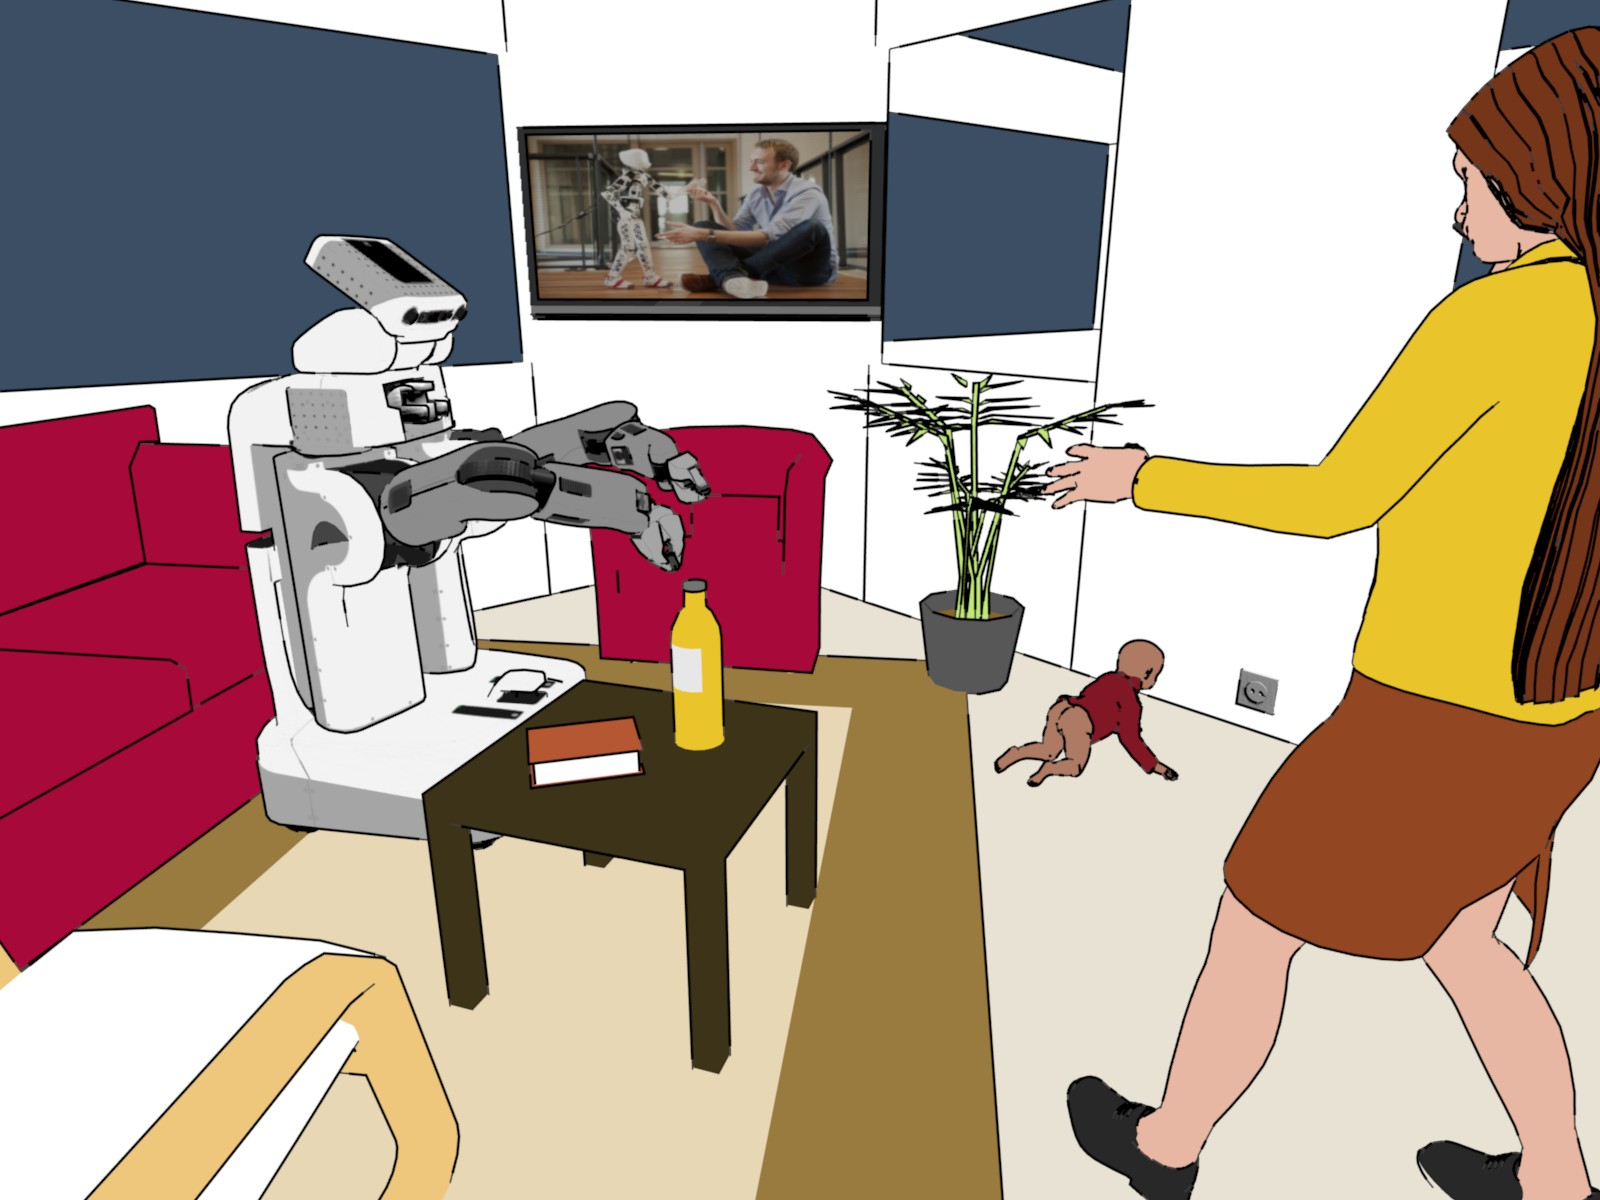
\includegraphics[width=\linewidth]{pr2-baby-3}
            \end{center}
        \end{column}
    \end{columns}

    \pause

    \vspace{2em}
    My PhD: a symbolic approach to this problem
\end{frame}


%%%%%%%%%%%%%%%%%%%%%%%%%%%%%%%%%%%%%%%%%%%%%%%%%%%%%%%%

{
    \paper{Lemaignan et al., {\bf Artificial Cognition for Social Human-Robot
    Interaction: An Implementation}, Artifical Intelligence, 2016}
\begin{frame}<3>{Multi-modal Symbolic situation assessment}

    \begin{columns}
        \begin{column}{0.4\linewidth}
        \centering
        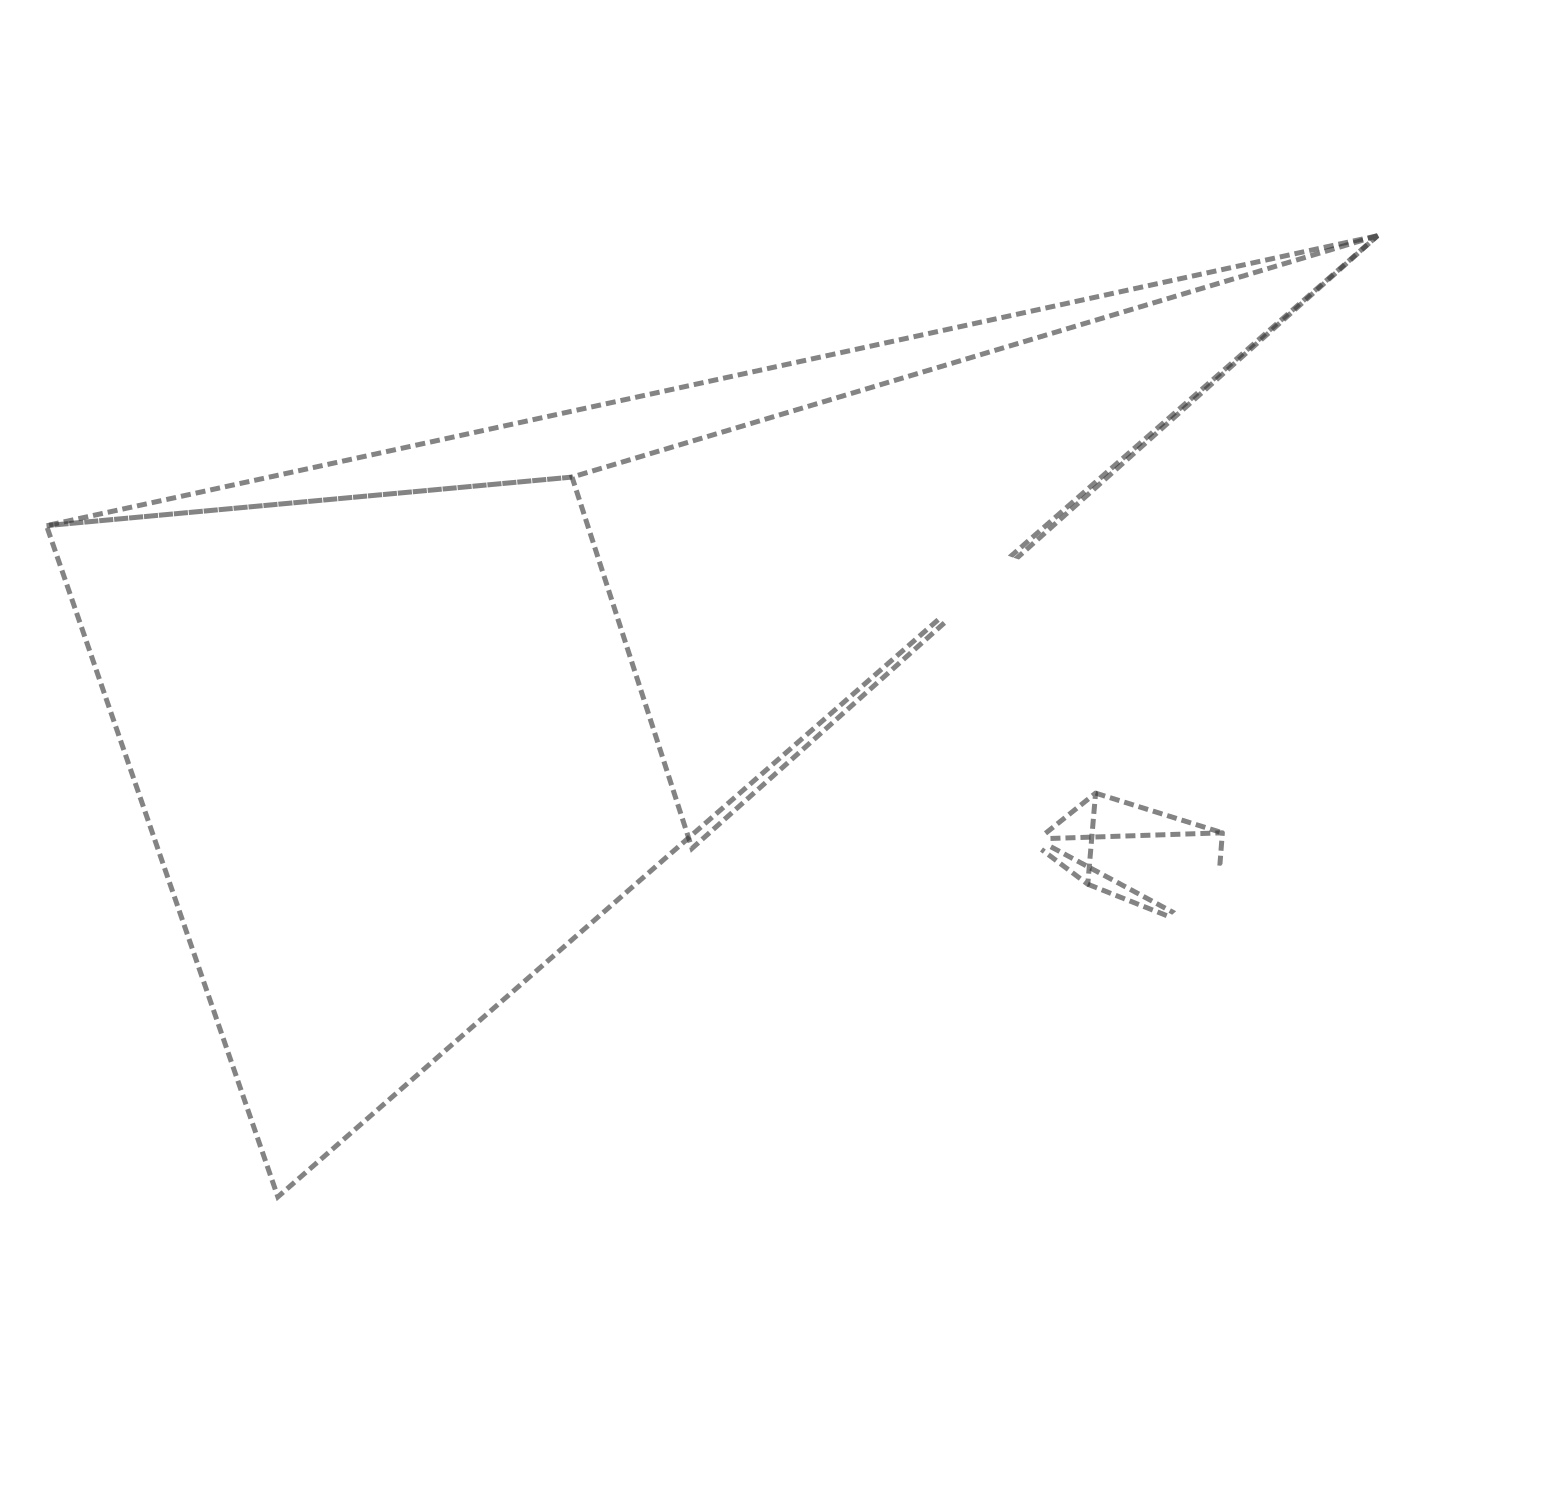
\includegraphics[width=\linewidth]{human-perspective-small}
             
        \end{column}
        \begin{column}{0.6\linewidth}
        
        \begin{figure}

        \resizebox{\columnwidth}{!}{%
        \begin{tikzpicture}[
            yscale=1.3,
            >=latex,
            every edge/.style={<-, draw, very thick},
            every node/.style={draw, font=\sf, node distance=0.5, rounded corners,
            align=center, inner sep=5pt,fill=hriSec2Dark!50},
            classof/.style={<-, draw=black!60, dashed},
            property/.style={<-, draw=hriSec2Comp},
            propname/.style={above, draw=none, fill=none, font=\tt, inner sep=2pt},
            instance/.style={draw=hriSec1Dark, font=\sf, node distance=0.5, rounded corners,
        align=center, inner sep=5pt, fill=none}]

            \node[fill=hriSec2Comp!50] (thing) {\textbf{thing}};
            \node [fill=hriSec3CompDark!50, node distance=1.8, below left=of
            thing](sthing) {place} edge[dashed] (thing);
            \node [fill=hriSec3CompDark!50, below left=of sthing] (agent) {agent} edge (sthing);
                \node [fill=hriSec3CompDark!50, below=of sthing] (artifact) {artifact} edge (sthing);
                \node [fill=hriSec3CompDark!50, below right=of sthing] (location) {physical
                support} edge (sthing);
                \node [fill=hriSec3CompDark!50, below right=of artifact] (table) {table}
                    edge (location) edge (artifact);


            \node [node distance=1, below right=of thing] (tthing) {temporal thing} edge (thing);
                \node [below right=of tthing] (evt) {event} edge[dashed] (tthing);
                            \node [below right=of evt] (act) {action} edge (evt);

        \uncover<2->{
        \draw[dotted, thick] (-8,-3.8) -- +(16, 0);

        \node [instance, below=3 of agent] (human) {human\_1} edge[classof, bend left] (agent);
        \node [instance, above left=of human] (human2) {human\_2} edge[classof, bend left] (agent);
        \node [instance, above right=of human, anchor=south] (robot) {myself} edge[classof, bend left] (agent);
        \node [instance, right=of human, anchor=north west] (book) {book\_game\_thrones}
        edge[classof] (artifact);
        \node [instance, right=2 of robot] (ikea) {ikea\_table} edge[classof, bend
        right] (table);
        \node [instance, right=2 of book] (brown) {brown} edge[property] node[propname] {hasColor} (book);


        }
        \uncover<3>{
        \draw[dotted, thick] (-8,-6.2) -- +(16, 0);

        \node [instance, below=5 of act] (moving) {move\_act\_42} edge[classof] (act);
        \path (moving.west) edge [property, out=180, in=-80, looseness=1] node[propname,below] {currentlyPerforms} (human.230);
        \path (human.280) edge [property, out=-80, in=-90, looseness=3.5] node[propname,right] {looksAt} (robot.south);
        \path (ikea.south) edge [property, out=-90, in=-80, looseness=2.5] node[propname, auto] {isOn} (book.320);
        }
        \end{tikzpicture}
        }

        \end{figure}

       \end{column}
    \end{columns}



        \badge{europe_phd}
\end{frame}
}

%%%%%%%%%%%%%%%%%%%%%%%%%%%%%%%%%%%%%%%%%%%%%%%%%%%%%%%%
%
%{
%\paper{Lemaignan et al. {\bf Grounding the Interaction: Anchoring
%Situated Discourse in Everyday HRI} Intl. J. of Social Robotics 2011}
%\begin{frame}{Dialogue Grounding}
%    \centering
%
%    I keep the NLP details for the questions, but:\\
%
%    \begin{columns}
%        \begin{column}{0.65\linewidth}
%
%    \centering
%    \vspace*{2em}
%    {\bf ``Give me the book on the table''}\\
%
%    \uncover<2-> {
%        $\downarrow$\\
%        {\tt me} $\rightarrow$ {\tt human\_1} \\
%        find({\tt\scriptsize ?obj type table}) $\rightarrow$ {\tt ikea\_table} \\
%        find({\tt\scriptsize ?obj type book, ?obj isOn ikea\_table})
%        $\rightarrow$ {\tt book\_game\_thrones} \\
%    }
%
%    \uncover<3-> {
%        $\downarrow$\\
%        { \tt
%            \textbf{human\_1} desires \textbf{give\_act\_1}, \\
%            \textbf{give\_act\_1} type \textbf{Give}, \\
%            \textbf{give\_act\_1} performedBy \textbf{myself}, \\
%            \textbf{give\_act\_1} actsOnObject \textbf{book}, \\
%            \textbf{give\_act\_1} receivedBy \textbf{human\_1} \\
%        }
%    }
%            
%        \end{column}
%        \begin{column}{0.35\linewidth}
%         \resizebox{\linewidth}{!}{%
% 
% 
%             \begin{tikzpicture}[
%                     >=latex,
%                 every edge/.style={draw, very thick},
%                 skill/.style={draw, rounded corners, align=center, inner sep=5pt, fill=black!20},
%                 label/.style={midway, align=center, font=\scriptsize, above},
%                 subpart/.style={rounded corners, draw, align=center, font=\scriptsize, fill opacity=0.5, text opacity=1, fill=white!50}]
% 
%             %%% PARSING
% 
%             \node at (0,0)[skill, fill=hriSec3CompDark!50] (prepro) {Pre-processing};
%                 \node [left=0.7 of prepro] (input) {\textbf{Input}};
%                 \path (input) edge [->] (prepro);
% 
%                 %\path (spark.100) edge [->, bend right] node[label] {symbolic \\ facts} (oro);
%                 \node [below =0.4 of prepro, skill, fill=hriSec3CompDark!50] (parsing) {Parsing};
%                 \path (prepro) edge [->] (parsing);
% 
%                 \coordinate (base-onto) at (4,0);
% 
%                 %%% RESOLUTION
%                     \node [below=0.4 of parsing, skill, fill=hriSec3!50, minimum height=4cm, minimum width=5cm] (resolution) {};
%                 \node [subpart, below=0.2 of resolution.115] (pron) {Pronouns \& \\ anaphora resolution};
%                 \node [subpart, below=0.2 of pron] (noun) {Noun phrase \\ resolution};
%                 \node [subpart, right=0.3 of noun, anchor=north west] (discr) {Discrimination};
%                 \node [subpart, below=0.2 of noun] (verb) {Verbal phrase \\ resolution};
%                 \node [subpart, cylinder, shape border rotate=90, aspect=0.5, below=0.2 of discr] (actions) {Actions};
%                 \path (pron) edge [->] (noun);
%                 \path (noun) edge [->] (discr);
%                 \path (noun) edge [->] (verb);
%                 \path (verb) edge [dashed, <->] (actions);
%                 \path (pron) edge [dashed, <->] node[label] {queries} (pron -| base-onto);
%                 \path (noun.20) edge [dashed, <->] node[label] {queries} (noun.20 -| base-onto);
%                 \path (discr) edge [<->] (discr -| base-onto);
% 
%                 \node [left=0.2 of resolution.west, rotate=90, anchor=south] {Resolution};
%                 \path (parsing) edge [->] (pron);
% 
%             %%% INTERPRETATION
%                     \node [skill, below=0.4 of resolution,minimum width=5cm, minimum height=3cm] (interp) {};
%                 \node [subpart, below=0.2 of interp.north] (content) {Content analysis};
%                 \node [below=0.6 of content.south west, subpart] (question) {Question \\ handler};
%                 \node [below=0.6 of content.south east, subpart] (stat) {Statement \\ builder};
%                 \path (content) edge [->] node[label, left] {question} (question);
%                 \path (content) edge [->] node [label, right] {goal | statement} (stat);
%                 \path (stat) edge [->] node [label] {asserts} (stat -| base-onto);
% 
%                 \node [left=0.2 of interp.west, rotate=90, anchor=south] {Interpretation};
% 
%                 \path (verb) edge [->] (content);
%                 \path (question) edge [dashed, bend right, <->] node[label] {queries} (question.south -| base-onto);
% 
%             %%% ONTOLOGY
%                     \node at (resolution.north -| base-onto) [rotate=-90, skill, minimum height=2cm, minimum width=7cm, fill=hriSec3!50, anchor=south west] (onto) {Ontology server};
% 
% 
%             %%% VERBALIZATION
%                 \node [below=0.7 of interp, skill, fill=hriSec2Dark!50] (verb) {Verbalization};
%             \path (question) edge [->] (verb);
%             \path (stat) edge [->] (verb);
%             \path (discr.south east) edge [black!50, dashed, bend left, <->] (verb.north east);
%             \node [right=0.7 of verb] (output) {\textbf{Output}};
%             \path (verb) edge [->] (output);
%         \end{tikzpicture}
%         }
%
%        \end{column}
%    \end{columns}
%
%        \badge{europe_phd}
%\end{frame}
%}
%
%%%%%%%%%%%%%%%%%%%%%%%%%%%%%%%%%%%%%%%%%%%%%%%%%%%%%%%%%
%
%{
%    \paper{Lemaignan et al., {\bf Artificial Cognition for Social Human-Robot
%    Interaction: An Implementation}, Artifical Intelligence, 2016}
%\begin{frame}{Multi-modal interaction}
%
%    \begin{columns}
%        \begin{column}{0.4\linewidth}
%        \centering
%        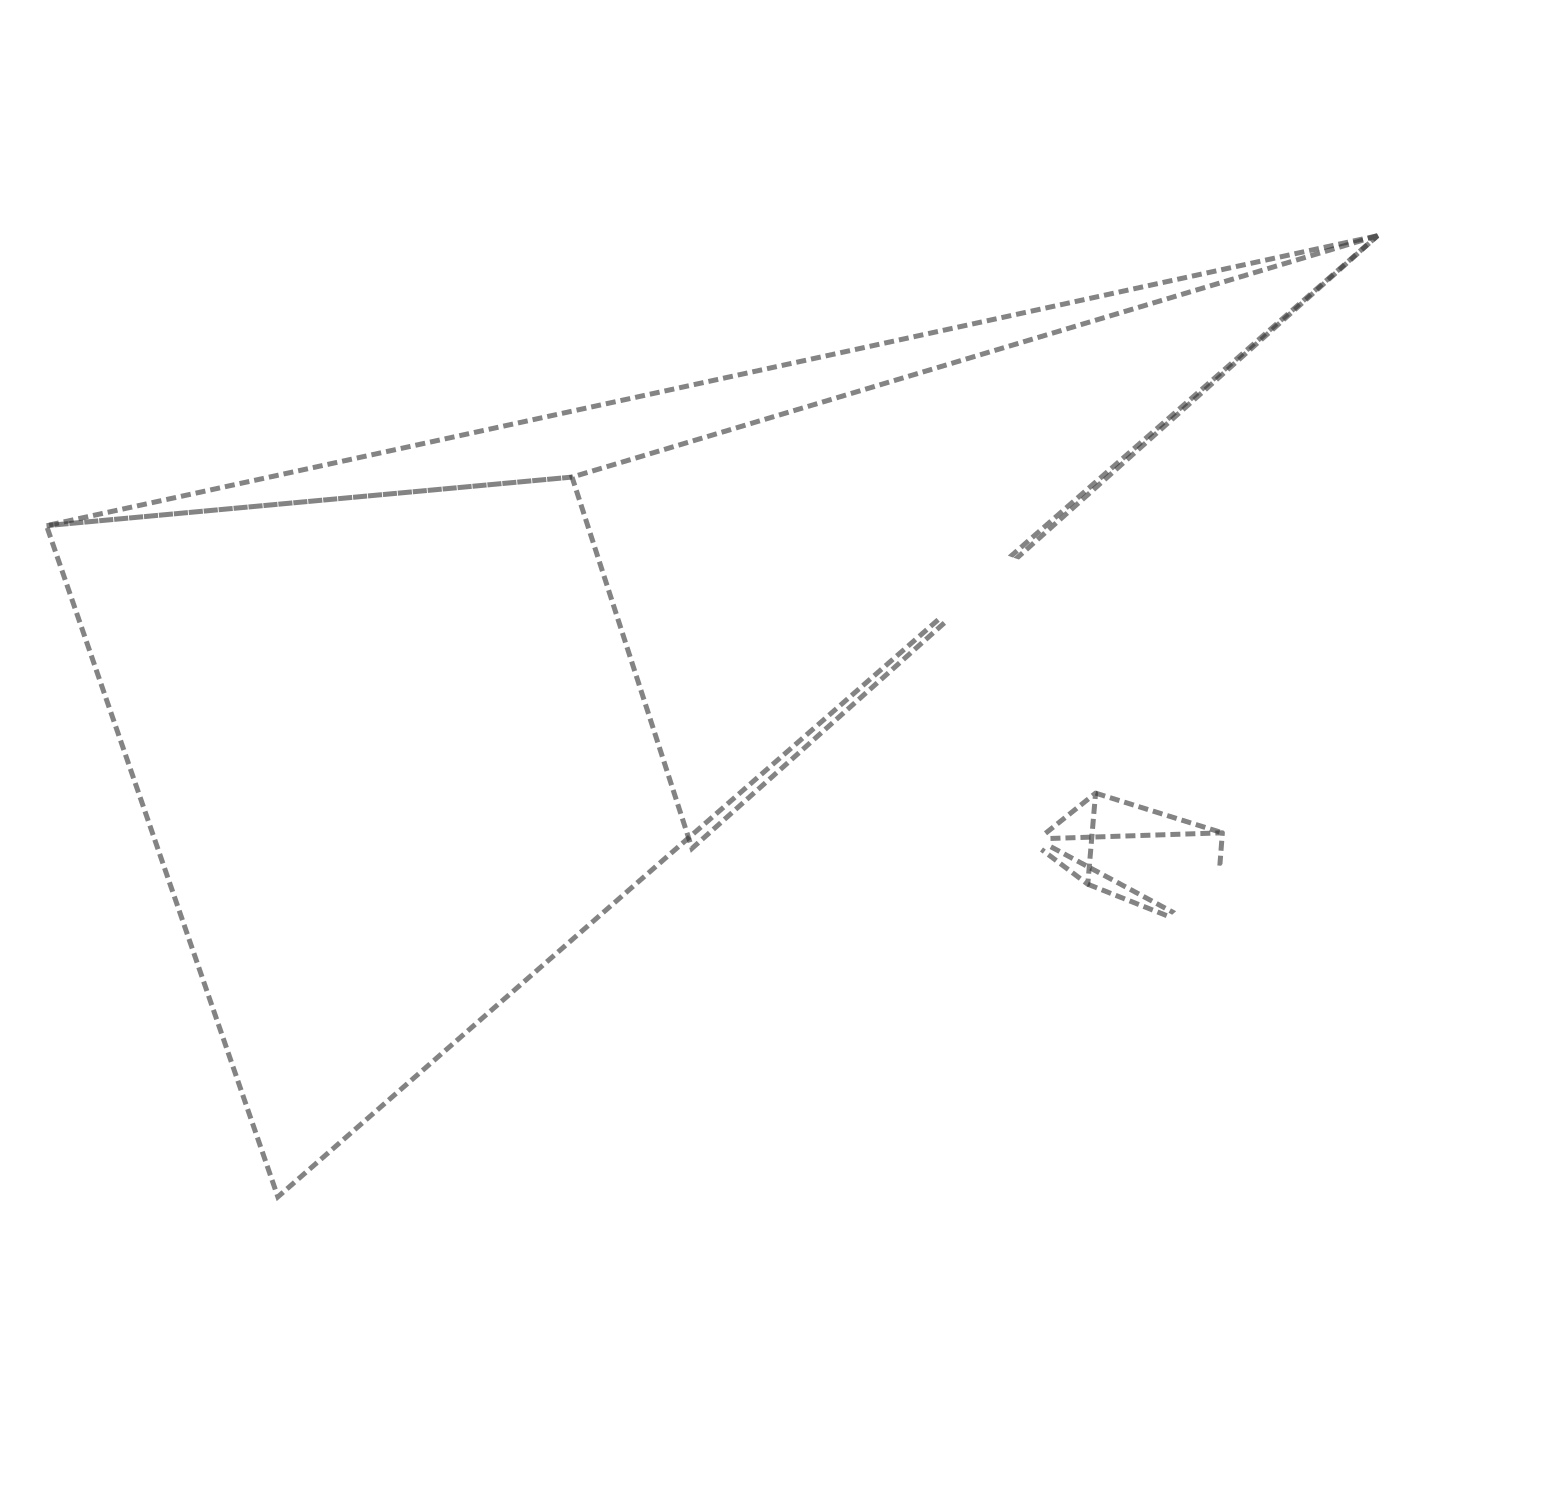
\includegraphics[width=\linewidth]{human-perspective-small}
%             
%        \end{column}
%        \begin{column}{0.6\linewidth}
%        
%    \centering
%    What about
%
%    {\bf ``Give me \emph{that} book''}?
%
%     \footnotesize
%    (or even: {\bf ``Give me \emph{that}!''})
%
%       \end{column}
%    \end{columns}
%
%
%
%        \badge{europe_phd}
%\end{frame}
%}

\videoframe[0.56]{videos/this_box.webm}
%\videoframe[0.56]{videos/this_box.webm?autostart&start=1}


%%%%%%%%%%%%%%%%%%%%%%%%%%%%%%%%%%%%%%%%%%%%%%%%%%%%%%%%%
%
%\section{One step further: Theory of Mind}
%
%%%%%%%%%%%%%%%%%%%%%%%%%%%%%%%%%%%%%%%%%%%%%%%%%%%%%%%%%
%
%\begin{frame}[plain]
%
%    \begin{center}
%        
\includegraphics[width=0.8\linewidth]{videos/this_box_thumb}
%
%        What if I ask for the video tape in the box, but the robot previously
%        moved it somewhere else?
%
%
%    \pause
%
%        {\bf False-belief situation}
%    \end{center}
%\end{frame}
%
%%%%%%%%%%%%%%%%%%%%%%%%%%%%%%%%%%%%%%%%%%%%%%%%%%%%%%%%%
%
%\begin{frame}{The False-Belief Experiment}
%    \centering
%    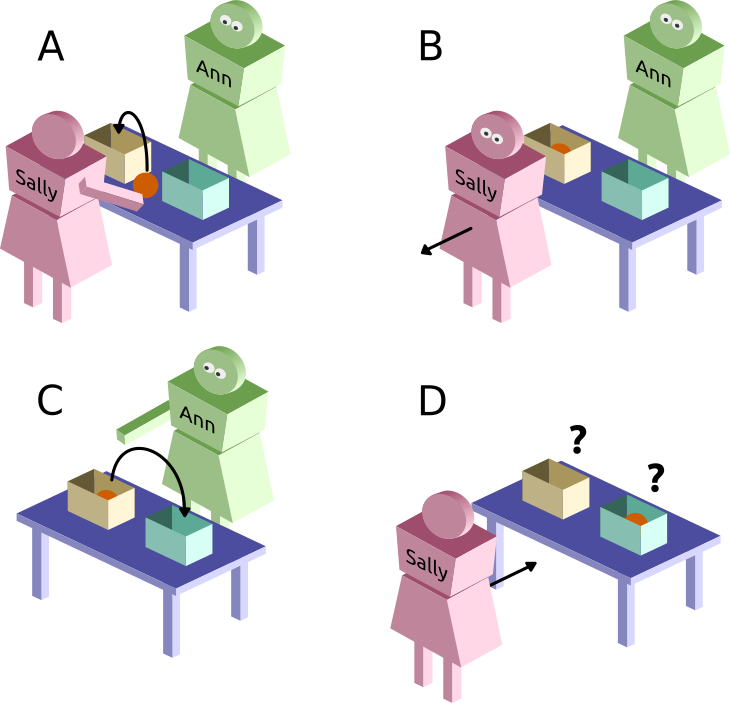
\includegraphics[width=0.7\textwidth]{sally_ann.pdf}
%
%\end{frame}
%
%%%%%%%%%%%%%%%%%%%%%%%%%%%%%%%%%%%%%%%%%%%%%%%%%%%%%%%%%

{
\paper{Ros, Lemaignan et al., {\bf Which One? Grounding the Referent Based on Efficient HRI}, ROMAN 2010}
\begin{frame}{Multiple Symbolic Models}
        \begin{multicols}{2}
            \begin{figure}
                \resizebox{0.4\textwidth}{!}{
                    \begin{tikzpicture}[
                        >=latex,
                        every edge/.style={<-, draw, very thick},
                        every node/.style={draw, font=\sf, node distance=0.5, rounded corners,
                                        align=center, inner sep=5pt,fill=hriSec2Dark!50},
                        classof/.style={<-, draw=black!60, dashed},
                        property/.style={<-, draw=hriSec2Comp},
                        propname/.style={above, draw=none, fill=none, font=\tt, inner sep=2pt},
                        instance/.style={draw=hriSec1Dark, font=\sf, node distance=0.5, rounded corners,
                        align=center, inner sep=5pt, fill=white}]

                    \node[fill=hriSec2Comp!50] (thing) {\textbf{thing}};
                    \node [fill=hriSec3CompDark!50, node distance=1.8, below left=of thing](sthing) {place} edge[dashed] (thing);
                    \node [fill=hriSec3CompDark!50, below left=of sthing] (agent) {agent} edge (sthing);
                        \node [fill=hriSec3CompDark!50, below=of sthing] (artifact) {artifact} edge (sthing);
                        \node [fill=hriSec3CompDark!50, below right=of sthing] (location) {physical
                        support} edge (sthing);
                        \node [fill=hriSec3CompDark!50, below right=of artifact] (table) {table}
                            edge (location) edge (artifact);


                    \node [node distance=1, below right=of thing] (tthing) {temporal thing} edge (thing);
                        \node [below right=of tthing] (evt) {event} edge[dashed] (tthing);
                                    \node [below right=of evt] (act) {action} edge (evt);

                \draw[dotted, thick] (-7,-5) -- (7.5, -5);

                \node [instance, below=3 of agent] (human) {human\_1} edge[classof, bend left] (agent);
                \node [instance, above left=of human] (human2) {human\_2} edge[classof, bend left] (agent);
                \node [instance, above right=of human, anchor=south] (robot) {pr2\_robot} edge[classof, bend left] (agent);
;
                \node [instance, right=of human, anchor=north west] (book) {book\_game\_thrones}
                edge[classof] (artifact);
                \node [instance, right=3 of robot] (ikea) {ikea\_table} edge[classof, bend
                right] (table);
                \node [instance, right=2 of book] (red) {red} edge[property] node[propname] {hasColor} (book);

                \node [instance,right=1 of robot,fill=hriSec2] {myself} edge[property] node[propname, auto,above] {$\equiv$} (robot);

                \draw[dotted, thick] (-7,-8) -- (7.5, -8);

                \path (book.200) edge [property, out=-100, in=-80, looseness=2]
                node[propname,auto] {isNextTo} (human.south);
                \path (book.270) edge [property, out=-100, in=-90, looseness=3.5] node[propname,auto] {looksAt} (robot.south);
                \path (ikea.south) edge [property, out=-90, in=-80, looseness=3] node[propname, auto] {isOn} (book.320);
                \end{tikzpicture}
            }

            \end{figure}
            \begin{figure}
                \resizebox{0.4\textwidth}{!}{
                    \begin{tikzpicture}[
                        >=latex,
                        every edge/.style={<-, draw, very thick},
                        every node/.style={draw, font=\sf, node distance=0.5, rounded corners,
                                        align=center, inner sep=5pt,fill=hriSec2Dark!50},
                        classof/.style={<-, draw=black!60, dashed},
                        property/.style={<-, draw=hriSec2Comp},
                        propname/.style={above, draw=none, fill=none, font=\tt, inner sep=2pt},
                        instance/.style={draw=hriSec1Dark, font=\sf, node distance=0.5, rounded corners,
                        align=center, inner sep=5pt, fill=white}]

                    \node[fill=hriSec2Comp!50] (thing) {\textbf{thing}};
                    \node [fill=hriSec3CompDark!50, node distance=1.8, below left=of thing](sthing) {place} edge[dashed] (thing);
                    \node [fill=hriSec3CompDark!50, below left=of sthing] (agent) {agent} edge (sthing);
                        \node [fill=hriSec3CompDark!50, below=of sthing] (artifact) {artifact} edge (sthing);
                        \node [fill=hriSec3CompDark!50, below right=of sthing] (location) {physical
                        support} edge (sthing);
                        \node [fill=hriSec3CompDark!50, below right=of artifact] (table) {table}
                            edge (location) edge (artifact);


                    \node [node distance=1, below right=of thing] (tthing) {temporal thing} edge (thing);
                        \node [below right=of tthing] (evt) {event} edge[dashed] (tthing);
                                    \node [below right=of evt] (act) {action} edge (evt);

                \draw[dotted, thick] (-7,-5) -- (7.5, -5);

                \node [instance, below=3 of agent] (human) {human\_1} edge[classof, bend left] (agent);
                \node [instance, above left=of human] (human2) {human\_2} edge[classof, bend left] (agent);
                \node [instance, above right=of human, anchor=south] (robot) {pr2\_robot} edge[classof, bend left] (agent);
;
                \node [instance, right=of human, anchor=north west] (book) {book\_game\_thrones}
                edge[classof] (artifact);
                \node [instance, right=3 of robot] (ikea) {ikea\_table} edge[classof, bend
                right] (table);
                \node [instance, right=2 of book] (red) {red} edge[property] node[propname] {hasColor} (book);

                \node [instance,below left=1 of human,fill=hriSec2] {myself} edge[property] node[propname, auto,above] {$\equiv$} (human);

                \draw[dotted, thick] (-7,-8) -- (7.5, -8);

                \path (book.200) edge [property, out=-100, in=-80, looseness=2]
                node[propname,auto] {isNextTo} (human.south);
                \path (book.270) edge [property, out=-100, in=-90, looseness=3.5] node[propname,auto] {looksAt} (robot.south);
                \path (ikea.south) edge [property, out=-90, in=-80, looseness=3] node[propname, auto] {isOn} (book.320);
                \end{tikzpicture}
            }
            \end{figure}
            \begin{figure}
                \resizebox{0.4\textwidth}{!}{
                    \begin{tikzpicture}[
                        >=latex,
                        every edge/.style={<-, draw, very thick},
                        every node/.style={draw, font=\sf, node distance=0.5, rounded corners,
                                        align=center, inner sep=5pt,fill=hriSec2Dark!50},
                        classof/.style={<-, draw=black!60, dashed},
                        property/.style={<-, draw=hriSec2Comp},
                        propname/.style={above, draw=none, fill=none, font=\tt, inner sep=2pt},
                        instance/.style={draw=hriSec1Dark, font=\sf, node distance=0.5, rounded corners,
                        align=center, inner sep=5pt, fill=white}]

                    \node[fill=hriSec2Comp!50] (thing) {\textbf{thing}};
                    \node [fill=hriSec3CompDark!50, node distance=1.8, below left=of thing](sthing) {place} edge[dashed] (thing);
                    \node [fill=hriSec3CompDark!50, below left=of sthing] (agent) {agent} edge (sthing);
                        \node [fill=hriSec3CompDark!50, below=of sthing] (artifact) {artifact} edge (sthing);
                        \node [fill=hriSec3CompDark!50, below right=of sthing] (location) {physical
                        support} edge (sthing);
                        \node [fill=hriSec3CompDark!50, below right=of artifact] (table) {table}
                            edge (location) edge (artifact);


                    \node [node distance=1, below right=of thing] (tthing) {temporal thing} edge (thing);
                        \node [below right=of tthing] (evt) {event} edge[dashed] (tthing);
                                    \node [below right=of evt] (act) {action} edge (evt);

                \draw[dotted, thick] (-7,-5) -- (7.5, -5);

                \node [instance, below=3 of agent] (human) {human\_1} edge[classof, bend left] (agent);
                \node [instance, above left=of human] (human2) {human\_2} edge[classof, bend left] (agent);
                \node [instance, above right=of human, anchor=south] (robot) {pr2\_robot} edge[classof, bend left] (agent);
;
                \node [instance, right=of human, anchor=north west] (book) {book\_game\_thrones}
                edge[classof] (artifact);
                \node [instance, right=3 of robot] (ikea) {ikea\_table} edge[classof, bend
                right] (table);
                \node [instance, right=2 of book] (red) {red} edge[property] node[propname] {hasColor} (book);

                \node [instance,below=1 of human2,fill=hriSec2] {myself} edge[property] node[propname, auto] {$\equiv$} (human2);

                \draw[dotted, thick] (-7,-8) -- (7.5, -8);

                \path (book.200) edge [property, out=-100, in=-80, looseness=2]
                node[propname,auto] {isNextTo} (human.south);
                \path (book.270) edge [property, out=-100, in=-90, looseness=3.5] node[propname,auto] {looksAt} (robot.south);
                \path (ikea.south) edge [property, out=-90, in=-80, looseness=3] node[propname, auto] {isOn} (book.320);
                \end{tikzpicture}
            }
            \end{figure}
            {\vspace*{1.5cm}\hspace*{2.5cm}\huge...}
        \end{multicols}
        \badge{europe_phd}
\end{frame}
}

%%%%%%%%%%%%%%%%%%%%%%%%%%%%%%%%%%%%%%%%%%%%%%%%%%%%%%%%

\videoframe[0.56]{videos/dialogs.webm}

%%%%%%%%%%%%%%%%%%%%%%%%%%%%%%%%%%%%%%%%%%%%%%%%%%%%%%%%%
%
%{
%    \paper{Lemaignan et al., {\bf Artificial Cognition for Social Human-Robot
%    Interaction: An Implementation}, Artifical Intelligence, 2016}
%\begin{frame}<6-7>{Into an control architecture}
%    \begin{figure}
%        \centering
%
%        \resizebox{0.9\paperwidth}{!}{%
%
%            
%            \alt<7>{\newcommand{\dimming}{10}}{\newcommand{\dimming}{50}}
%
%            \tikzset{subpart/.style={draw, font=\scriptsize, fill opacity=0.5, text opacity=1, fill=white!50}}
%
%            \begin{tikzpicture}[
%                    >=latex,
%                    every edge/.style={draw, very thick},
%                    skill/.style={draw, rounded corners, align=center, inner sep=5pt, fill=black!20},
%                label/.style={midway, align=center, font=\scriptsize, fill=white}]
%
%                %%% Separation between deliberative layer and sensori-motor layer
%                \draw[dotted, thick] (-8,-5) -- (12, -5);
%
%                %%% SPARK
%                \uncover<2->{
%                    \node at (4,-3.5)[skill, fill=hriSec3!\dimming] (spark) {%
%                    \begin{tikzpicture}
%                        \node at (0,0) (geom) {Geometric \& Temporal Reasoning -- {\tt spark}};
%                        \node [subpart, below=0.2 of geom.south west, anchor=north west] (world-update) {Sensors fusion};
%                        \node [subpart, right=0.2 of world-update] (geom-model) {Geometric model of the environment};
%                        \node [subpart, right=0.2 of geom-model] (fact-prod) {Symbolic facts production};
%                    \end{tikzpicture}
%                };
%                }
%
%                %%% LOWLEVEL
%                \node [skill, below=0.7 of spark,fill=gray!\dimming] (lowlevel) {%
%                    \begin{tikzpicture}
%                        \node at (0,0) (sensori) {Sensorimotor layer};
%                        %\node [subpart, below=0.2 of sensori.south west, anchor=north west, align=left] (perception) {{\bf Perception} \\ 2D markers, RGB-D, motion capture};
%                        %\node [subpart, align=right, right=0.2 of perception] {{\bf Actuation} \\ Head's pan-tilt unit, grippers, arms, wheels};
%                    \end{tikzpicture}
%                };
%
%                \uncover<2->{
%                \path (lowlevel) edge [->] (spark);
%                }
%
%                %%% ORO
%                \uncover<3->{
%                \node at (0,0)[skill, ultra thick, fill=hriSec2Dark!50] (oro)
%                {Symbolic facts \\ and beliefs management -- {\tt oro}};
%                \path (spark.100) edge [->, bend right] node[label] {symbolic \\ facts} (oro);
%                }
%
%                %%% HATP
%                \uncover<5->{
%                \node at (-6, 2.5)[skill, fill=hriSec1!\dimming] (hatp) {Human-aware
%                symbolic \\task planning -- {\tt hatp}};
%                \path (hatp) edge [<->, bend right] node[label] {world model and \\ agents beliefs} (oro.170);
%                }
%
%                %%% DIALOGS
%                \uncover<4->{
%                \node at (-6, -3) [skill, fill=hriSec3Dark!50] (dialogs)
%                {Dialogue processing\\{\tt dialogs}};
%                \path (dialogs) edge [<->, bend left] node[label] {natural language \\ grounding} (oro.190);
%                }
%                %%% SHARY
%                \uncover<5->{
%                \node at (4,4.5)[skill, fill=hriSec1Comp!\dimming] (shary) {%
%                    \begin{tikzpicture}
%                        \node at (0,0) (exec) {Execution Controller -- {\tt shary} | {\tt pyrobots}};
%                        \node [subpart, below=0.2 of exec.south west, anchor=north west] (plans) {Goal \& Plans \\ management};
%                        \node [subpart, right=0.2 of plans] (sit-asses) {Situation assessment \\ and context management};
%                        \node [subpart, right=0.2 of sit-asses] {Action instantiation, \\ execution and monitoring};
%                    \end{tikzpicture}
%                };
%                \path (shary) edge [<->, bend left] node[label] {events, \\ world model and \\ agents beliefs} (oro);
%                \path (shary) edge [<->, bend left, looseness=0.8] node[label] {action monitoring \\ and management of \\ position hypotheses} (spark);
%                \path (shary.west) edge [<->, bend right] node[label] {shared \\ plans} (hatp);
%                }
%                %%% MHP
%                \uncover<6->{
%                \node at (9,0)[skill, fill=hriSec3CompDark!\dimming] (mhp) {Human-aware Motion \\ and Manipulation Planning\\{\tt mhp}};
%                \path (shary.340) edge [<->, bend left] node[label] {motion plan \\ requests} (mhp);
%                \path (spark.5) edge [->, bend right] node[label] {environment\\model} (mhp);
%                \path (lowlevel.east) edge [<-, bend right=60, looseness=1.3] node[label] {atomic\\actions} (mhp.south east);
%                }
%
%
%
%            \end{tikzpicture}
%        }
%    \end{figure}
%
%        \badge{europe_phd}
%\end{frame}
%}
%
%%%%%%%%%%%%%%%%%%%%%%%%%%%%%%%%%%%%%%%%%%%%%%%%%%%%%%%%%
%
%{
%\paper{Lemaignan et al. {\bf Artificial Cognition for Social Human-Robot
%     Interaction: An Implementation} Artifical Intelligence, 2016}
%\begin{frame}{One example}
%
%    \begin{center}
%
%     Walkthrough one full-stack example in the question
%     \vspace{2em}
%
%     \begin{columns}
%         \begin{column}{0.3\linewidth}
%                 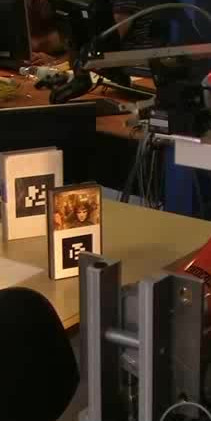
\includegraphics[height=0.6\paperheight]{clean-table}
%         \end{column}
%         \begin{column}{0.7\linewidth}
%             \centering
%             \resizebox{!}{0.6\paperheight}{%
%                 \begin{tikzpicture}[
%                         >=latex,
%                     every edge/.style={draw, ultra thick, ->},
%                     every node/.style={align=center},
%                     robot/.style={fill=hriSec2Comp!50},
%                     plan/.style={draw,
%                      thick,  
%                      circle, 
%                      font=\sf,
%                      align=center,
%                      fill=hriSec3CompDark!50, 
%                      minimum size=1cm, 
%                      inner sep=0.1cm}
%                  ]
%
%                     \coordinate (figbottom) at (-0.5, -28.5);
%
%
%                     \fill[gray!10!white] (4.6,.5) rectangle (figbottom);
%
%                     \path (-0.5,0) edge (figbottom) node[sloped, above left, rotate=90] {\large\bf time};
%
%                     \node at (2,0) (percept) {\bf Perception};
%                     \node[below=0.5 of percept.south west, anchor=mid] {camera};
%                     \node[below=0.5 of percept.south east, anchor=mid] {3D model};
%
%                     \node[right=4 of percept, minimum width=2.5cm] (kb) {\bf Knowledge};
%                     \node[below=0.5 of kb.south west, anchor=mid east] (kbr) {robot};
%                     \node[below=0.5 of kb.south east, anchor=mid west] (kbh) {human};
%                     \draw[dotted] (kbr) to (figbottom -| kbr);
%                     \draw[dotted] (kbh) to (figbottom -| kbh);
%
%                     \fill[gray!10!white] (12,.5) rectangle (17,0 |- figbottom);
%                     \node[right=4.5 of kb] (plan) {\bf Plan};
%                     \node[below=0.5 of plan.south west, anchor=mid east] (probot) {robot};
%                     \node[below=0.5 of plan.south east, anchor=mid west] (phuman) {human};
%                     \draw[dotted] (probot) to (figbottom -| probot);
%                     \draw[dotted] (phuman) to (figbottom -| phuman);
%
%                     \node[right=5 of plan] (action) {\bf Actions};
%                     \node[below=0.5 of action.south west, anchor=mid east] (arobot) {robot};
%                     \node[below=0.5 of action.south east, anchor=west] (ahuman) {human\\(monitoring)};
%                     \draw[dotted] (arobot) to (figbottom -| arobot);
%                     \draw[dotted] (ahuman) to (figbottom -| ahuman);
%
%                     \draw[dashed] (-0.6,-1.2) --(24, -1.2);
%
%                     \node[anchor=east] at (-0.5, -3) (t1) {\Large $t_1$};
%                     \node[anchor=east, below=6 of t1] (t2) {\Large $t_2$};
%                     \node[anchor=east, below=6 of t2] (t3) {\Large $t_3$};
%                     \node[anchor=east, below=4 of t3] (t4) {\Large $t_4$};
%                     \node[anchor=east, below=5 of t4] (t5) {\Large $t_5$};
%
%                     %%%%%%%%%%%%%%%%%%%%%%%%%%%%%%%%%%%%%%%%%%%%%%%%%%%%%%%%%%%%%%%%%%%%%%%%%%%%%%%%%%%%%%%%%%%%
%                     %%% PERCEPTIONS
%                     %%%%%%%%%%%%%%%%%%%%%%%%%%%%%%%%%%%%%%%%%%%%%%%%%%%%%%%%%%%%%%%%%%%%%%%%%%%%%%%%%%%%%%%%%%%%
%
%         \node at (t1 -| percept) (cam1) {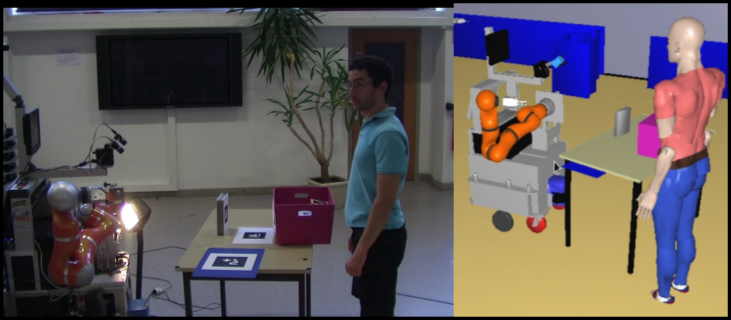
\includegraphics[height=2cm]{cleantable/manip_run_cam1.png}};
%         \node at (t2 -| percept) (cam2) {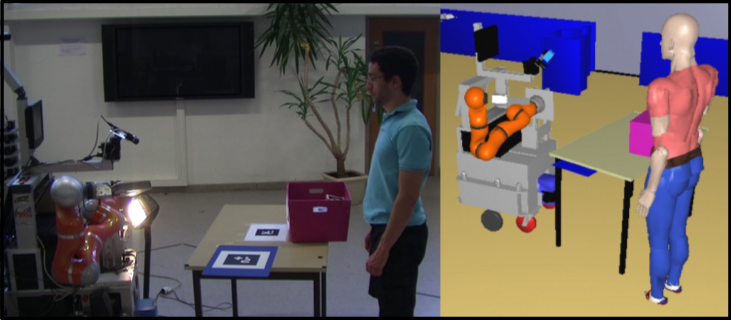
\includegraphics[height=2cm]{cleantable/manip_run_cam2.png}};
%         \node at (t3 -| percept) (cam3) {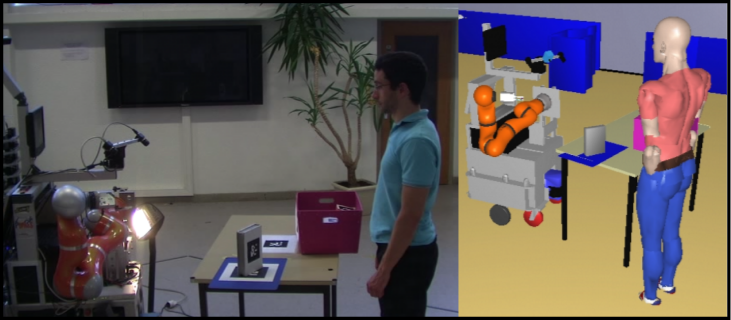
\includegraphics[height=2cm]{cleantable/manip_run_cam3.png}};
%         \node at (t4 -| percept) (cam4) {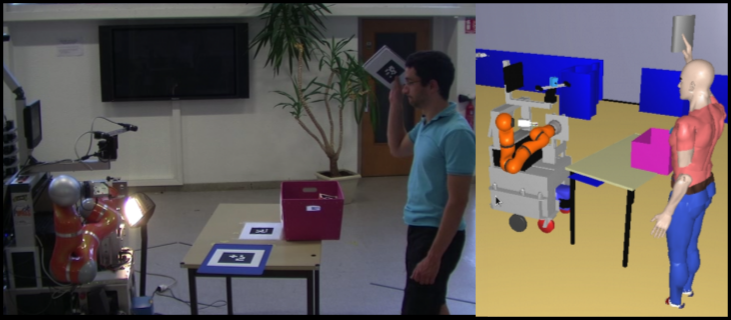
\includegraphics[height=2cm]{cleantable/manip_run_cam4.png}};
%         \node at (t5 -| percept) (cam5) {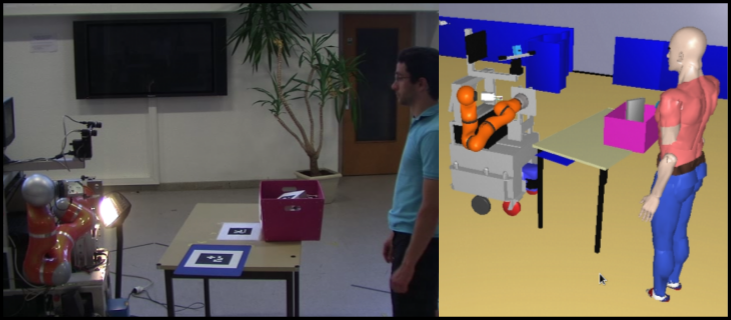
\includegraphics[height=2cm]{cleantable/manip_run_cam5.png}};
%
%         %%%%%%%%%%%%%%%%%%%%%%%%%%%%%%%%%%%%%%%%%%%%%%%%%%%%%%%%%%%%%%%%%%%%%%%%%%%%%%%%%%%%%%%%%%%%
%         %%% KNOWLEDGE
%         %%%%%%%%%%%%%%%%%%%%%%%%%%%%%%%%%%%%%%%%%%%%%%%%%%%%%%%%%%%%%%%%%%%%%%%%%%%%%%%%%%%%%%%%%%%%
%
%         \node[fill=white,align=left] at (cam1 -| kbr) (kb1) {\stmt{TAPE isVisible true}\\
%                                                    \stmt{TAPE isReachable true}\\
%                                                    \stmt{TAPE isOn TABLE}\\
%                                                    \stmt{BIN isVisible true}\\
%                                                    \stmt{BIN isReachable false}};
%
%         \node[fill=white,align=left] at (cam1 -| kbh) {\stmt{TAPE isVisible true}\\
%                                                    \stmt{TAPE isReachable false}\\
%                                                    \stmt{TAPE isOn TABLE}\\
%                                                    \stmt{BIN isVisible true}\\
%                                                    \stmt{BIN isReachable true}};
%
%         \node[fill=white,align=left] at (cam2 -| kbr) (kb2) {\stmt{ROBOT hasInHand TAPE}};
%
%
%         \node[fill=white,align=left] at (cam3 -| kbr) {\stmt{TAPE isReachable true}\\
%                                        \stmt{TAPE isVisible true} \\
%                                        \stmt{TAPE isOn TABLE}};
%
%         \node[fill=white,align=left ] at (cam3 -| kbh) (kb3) {\stmt{TAPE isReachable true}\\
%                                         \stmt{TAPE isVisible true}};
%
%         \node[fill=white,align=left] at (cam4 -| kbh) (kb4) {\stmt{HUMAN hasInHand TAPE}};
%
%         \node[fill=white,align=left] at (cam5 -| kbr)  {\stmt{TAPE isIn BIN}};
%         \node[fill=white,align=left] at (cam5 -| kbh) (kb5) {\stmt{TAPE isIn BIN}};
%
%         %%%%%%%%%%%%%%%% %%%%%%%%%%%%%%%%%%%%%%%%%%%%%%%%%%%%%%%%%%%%%%%%%%%%%%%%%%%%%%%%%%%%%%%%%%%%
%         %%% PLANS
%         %%%%%%%%%%%%%%%%%%%%%%%%%%%%%%%%%%%%%%%%%%%%%%%%%%%%%%%%%%%%%%%%%%%%%%%%%%%%%%%%%%%%%%%%%%%%
%
%         \node[fill=gray!10!white,below=1 of plan] (incoming) {\bf \Large Incoming goal \\ \it Clean the table!};
%
%         \node[anchor=north, plan, robot] at (cam1.south -| probot) (pr1) {\bf TAKE\\TAPE\\TABLE};
%         \node[anchor=north, plan, robot] at (cam2.south -| probot)  (pr2) {\bf PUTRV\\TAPE\\TABLE} edge[<-] (pr1);
%         \node[anchor=north, plan] at (cam3.south -| phuman) (ph1) {\bf TAKE\\TAPE\\TABLE} edge[<-] (pr2);
%         \node[anchor=north, plan]  at (cam4.south -| phuman) (ph2) {\bf PUT\\TAPE\\BIN} edge[<-] (ph1);
%
%         \node[fill=gray!10!white,anchor=north] at (cam5.south -| plan) (done) {\bf \Large Goal completed};
%
%         %%%%%%%%%%%%%%%%%%%%%%%%%%%%%%%%%%%%%%%%%%%%%%%%%%%%%%%%%%%%%%%%%%%%%%%%%%%%%%%%%%%%%%%%%%%%
%         %%% ACTIONS
%         %%%%%%%%%%%%%%%%%%%%%%%%%%%%%%%%%%%%%%%%%%%%%%%%%%%%%%%%%%%%%%%%%%%%%%%%%%%%%%%%%%%%%%%%%%%%
%
%         \only{
%             \node[fill=white] at (pr1 -| arobot) (ep1) {\it evaluate pre-conditions};
%
%         \node[below=0.1 of ep1] (mhp1) {%
%             \begin{tikzpicture}
%                 \node[fill=white] (title) {\bf motion planning};
%                 \node[below=0.1 of title.south west, label=below:{\tt PICK\_GOTO}] (mapg) {
\includegraphics{cleantable/MHP_ARM_PICK_GOTO}};
%                 \node[fill=white,right=of mapg, label=below:{\tt TAKE\_TO\_FREE}] (mattf) {
\includegraphics{cleantable/MHP_ARM_TAKE_TO_FREE}} edge[<-] (mapg);
%             \end{tikzpicture}
%         };
%         \node[fill=white,below=0.1 of mhp1] (me1) {\bf motion execution};
%         \node[fill=white,below=0.1 of me1] (ae1) {\it assess post-conditions};
%     }
%     %%%%%%%%%%%%%%%%%%%%%%%%%%%%%%%%%%%%%%%%%%%%%%%%%%%%%%%%%%%%%%%%%%%%%%%%%%%%%%%%%%%%%%%%%%%%%
%         \only{
%             \node[fill=white] at (pr2 -| arobot) (ep2) {\it evaluate pre-conditions};
%
%         \node[below=0.1 of ep2] (mhp2) {%
%             \begin{tikzpicture}
%                 \node[fill=white] (title) {\bf motion planning};
%                 \node[fill=white,below=0.1 of title, label=below:{\tt ESCAPE}] (maeo) {
\includegraphics{cleantable/MHP_ARM_ESCAPE_OBJECT}};
%                 \node[left=of maeo, label=below:{\tt PLACE\_FROM\_FREE}] (mapff) {
\includegraphics{cleantable/MHP_ARM_PLACE_FROM_FREE}} edge (maeo);
%                 \node[fill=white,right=of maeo, label=below:{\tt TO\_FREE}] (maf) {
\includegraphics{cleantable/MHP_ARM_FREE}} edge[<-] (maeo);
%             \end{tikzpicture}
%         };
%         \node[fill=white,below=0.1 of mhp2] (me2) {\bf motion execution};
%         \node[fill=white,below=0.1 of me2] (ae2) {\it assess post-conditions};
%     }
%     %%%%%%%%%%%%%%%%%%%%%%%%%%%%%%%%%%%%%%%%%%%%%%%%%%%%%%%%%%%%%%%%%%%%%%%%%%%%%%%%%%%%%%%%%%%%%
%
%         \node[anchor=north] at (ph1 -| ahuman) (wait1) {%
%             \begin{tikzpicture}
%                 \node[fill=white] (title) {\it wait for pick\\ {\tt TAPE} \it from {\tt TABLE}};
%                 \node[below=0.1 of title] {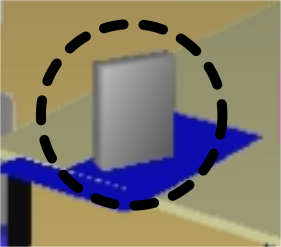
\includegraphics{cleantable/wait_for_pick}};
%             \end{tikzpicture}
%         };
%
%         \node[anchor=north] at (ph2 -| ahuman) (wait2) {%
%             \begin{tikzpicture}
%                 \node[fill=white] (title) {\it wait for put\\ {\tt TAPE} \it into {\tt BIN}};
%                 \node[below=0.1 of title] {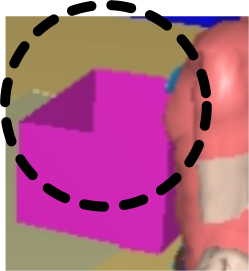
\includegraphics{cleantable/wait_for_throw}};
%             \end{tikzpicture}
%         };
%
%
%         %%%%%%%%%%%%%%%%%%%%%%%%%%%%%%%%%%%%%%%%%%%%%%%%%%%%%%%%%%%%%%%%%%%%%%%%%%%%%%%%%%%%%%%%%%%%
%         %%% FLOW
%         %%%%%%%%%%%%%%%%%%%%%%%%%%%%%%%%%%%%%%%%%%%%%%%%%%%%%%%%%%%%%%%%%%%%%%%%%%%%%%%%%%%%%%%%%%%%
%         \draw[dotted, ->, in=45, out=180] (incoming.west) to (kb1);
%         \draw[dotted, ->, bend right] (kb1) to (pr1);
%         \draw[dotted, ->, bend left] (pr1) to (ep1);
%         \draw[dotted, ->, in=45, out=180] (ae1.west) to (kb2);
%         \draw[dotted, ->, bend right] (kb2) to (pr2);
%         \draw[dotted, ->, bend left] (pr2) to (ep2);
%         \draw[dotted, ->, in=45, out=180] (ae2.west) to (kb3);
%         \draw[dotted, ->, bend right] (kb3) to (ph1);
%         \draw[dotted, ->, bend left] (ph1) to (wait1);
%         \draw[dotted, ->, in=-20, out=180] (wait1.west) to (kb4.east);
%         \draw[dotted, ->, bend right] (kb4) to (ph2);
%         \draw[dotted, ->, bend left] (ph2) to (wait2);
%         \draw[dotted, ->, in=20, out=180] (wait2.west) to (kb5);
%         \draw[dotted, ->, bend left] (kb5.east) to (done.north);
%
%
%     \end{tikzpicture}
%      }
%         \end{column}
%     \end{columns}
%    \end{center}
%
%\end{frame}
%}
%
%%%%%%%%%%%%%%%%%%%%%%%%%%%%%%%%%%%%%%%%%%%%%%%%%%%%%%%%%

\section*{Field Work}

%%%%%%%%%%%%%%%%%%%%%%%%%%%%%%%%%%%%%%%%%%%%%%%%%%%%%%%%

\imageframe[color=black]{experiments}

%%%%%%%%%%%%%%%%%%%%%%%%%%%%%%%%%%%%%%%%%%%%%%%%%%%%%%%%

\imageframe[color=black]{cowriter/henry}

%%%%%%%%%%%%%%%%%%%%%%%%%%%%%%%%%%%%%%%%%%%%%%%%%%%%%%%%%
%{
%    \paper{Lemaignan et al. {\bf Learning by Teaching a Robot: The Case of Handwriting} -- Robotics and Automation Magazine 2016}
%
%\begin{frame}{The CoWriter project}
%    \badge{europe_epfl}
%
%    Can we address children' hand-writing impairments with robots?
%
%    \begin{itemize}
%        \item<2-> Robots do not know how to write!
%        \item<3-> Learning by Teaching
%        \item<4-> (nice side-effect: we can adapt to each child and each disabilities)
%    \end{itemize}
%\end{frame}
%}
%%%%%%%%%%%%%%%%%%%%%%%%%%%%%%%%%%%%%%%%%%%%%%%%%%%%%%%%

\videoframe[0.56]{figs/cowriter/training-s.mp4}

%%%%%%%%%%%%%%%%%%%%%%%%%%%%%%%%%%%%%%%%%%%%%%%%%%%%%%%%

%{
%    \paper{Hood, Lemaignan et al. {\bf When Children Teach a Robot to Write: An
%    Autonomous Teachable Humanoid [...]} -- HRI 2015}
%
%\begin{frame}{Learning from demonstration}
%    \begin{center}
%    
\includegraphics[width=0.8\textwidth]{cowriter/learningSdemo.png}
%    \end{center}
%\end{frame}
%
%}

%{
%    \paper{Lemaignan et al. {\bf Learning by Teaching a Robot: The Case of Handwriting} -- Robotics and Automation Magazine 2016}
%\begin{frame}{Learning to draw a 5}
%    \begin{center}
%        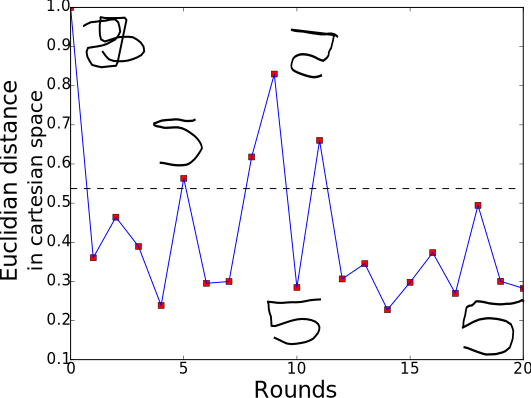
\includegraphics[width=0.8\linewidth]{cowriter/henry5}
%    \end{center}
%    \badge{europe_epfl}
%\end{frame}
%}

%%%%%%%%%%%%%%%%%%%%%%%%%%%%%%%%%%%%%%%%%%%%%%%%%%%%%%%%%
%\imageframe[color=black]{cowriter/diego-correct}
%
%\begin{frame}{Before -- After}
%    \begin{center}
%        \only<1-2>{
%        \includegraphics[width=0.43\linewidth]{cowriter/lettre-base}
%        \uncover<2>{
%            \hspace{1cm}%
%        \includegraphics[width=0.43\linewidth]{cowriter/lettre-final}
%        }
%        }
%        \only<3>{
%        \includegraphics[width=0.43\linewidth]{cowriter/lettre-base-highlight}
%            \hspace{1cm}%
%        \includegraphics[width=0.43\linewidth]{cowriter/lettre-final-highlight}
%        }
%    \end{center}
%        \badge{europe_epfl}
%\end{frame}

%%%%%%%%%%%%%%%%%%%%%%%%%%%%%%%%%%%%%%%%%%%%%%%%%%%%%%%%


%%%%%%%%%%%%%%%%%%%%%%%%%%%%%%%%%%%%%%%%%%%%%%%%%%%%%%%%

{
    \paper{Lemaignan et al. {\bf Learning by Teaching a Robot: The Case of Handwriting} -- Robotics and Automation Magazine 2016}


\begin{frame}{The Robot as a Social Agent}

    \begin{columns}
        \begin{column}{0.5\linewidth}
            \begin{center}
                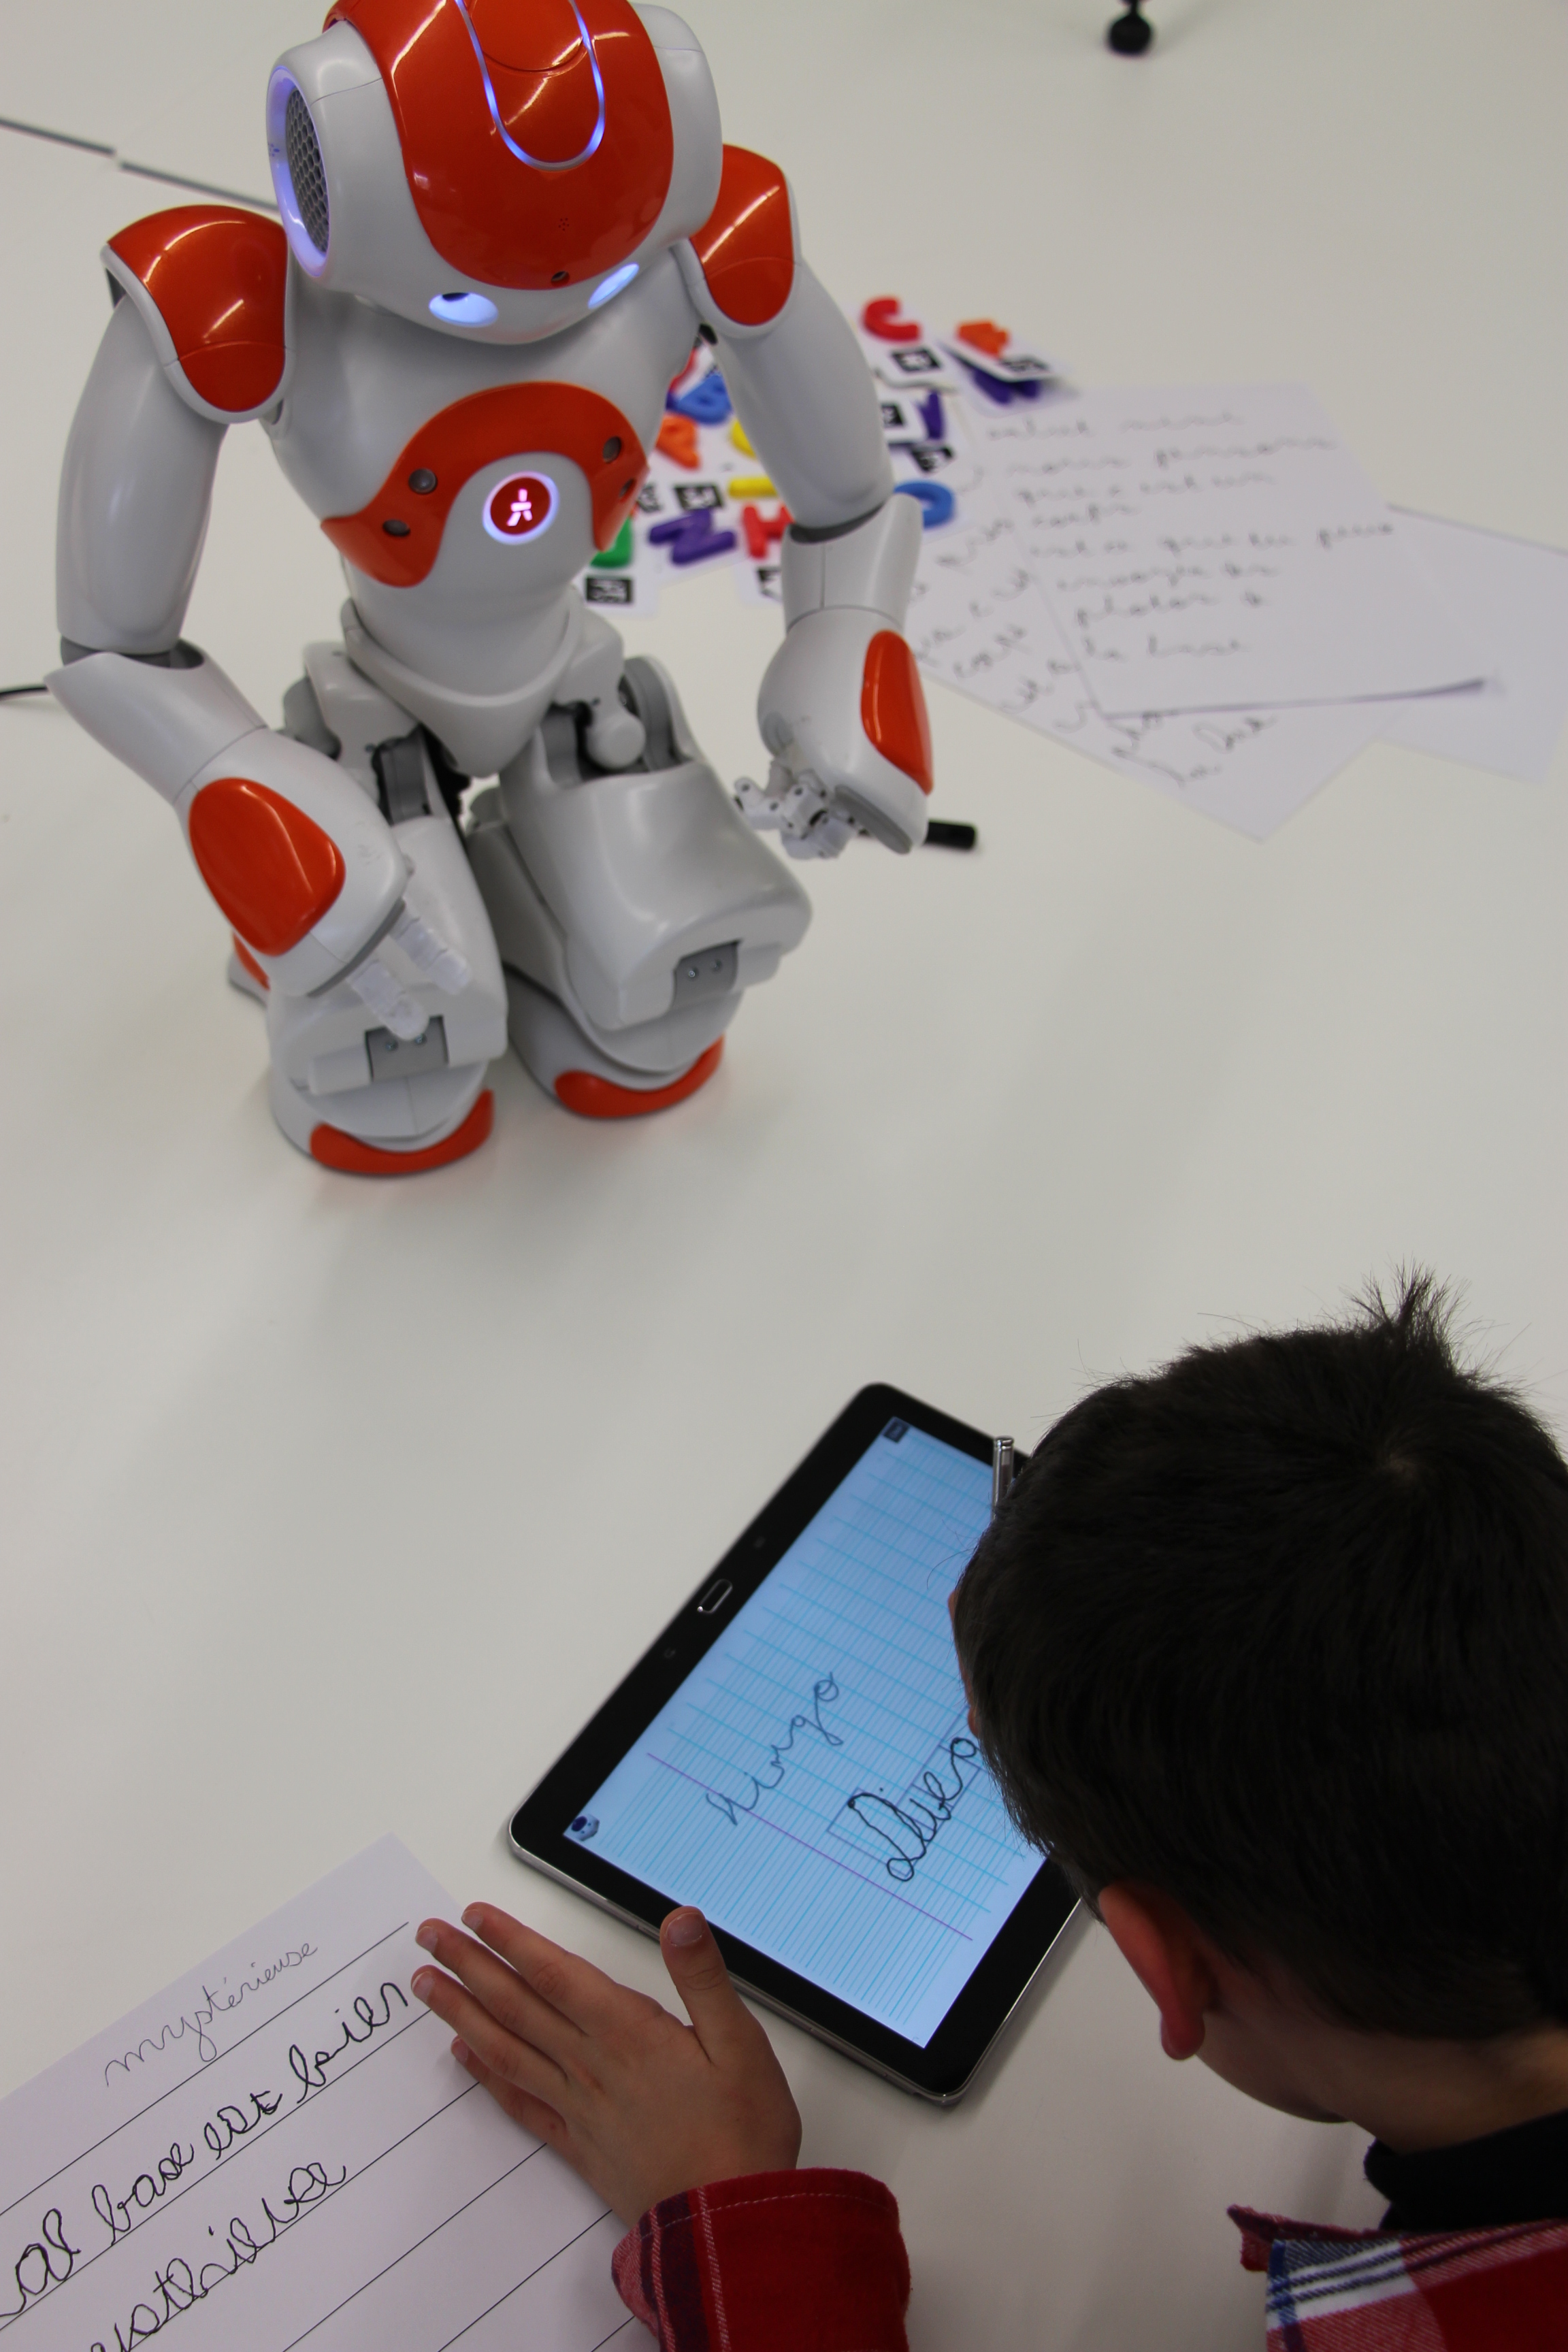
\includegraphics[width=0.8\linewidth]{cowriter/diego-correct}
            \end{center}
        \end{column}
        \begin{column}{0.5\linewidth}
                {\bf The robot as a cognitive agent is key here}
                    \begin{itemize}
                        \item Protégé effect
                        \item metacognition
                    \end{itemize}
        \end{column}
    \end{columns}
    \badge{europe_epfl}
\end{frame}
}

%%%%%%%%%%%%%%%%%%%%%%%%%%%%%%%%%%%%%%%%%%%%%%%%%%%%%%%%

\begin{frame}{Other experimental work}

        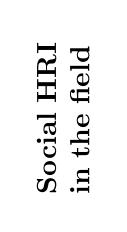
\begin{tikzpicture}
            \node[rotate=90,text width=2cm]{\textbf{Social HRI\\in the field}};
        \end{tikzpicture}
            \hyperlink{croquignole}{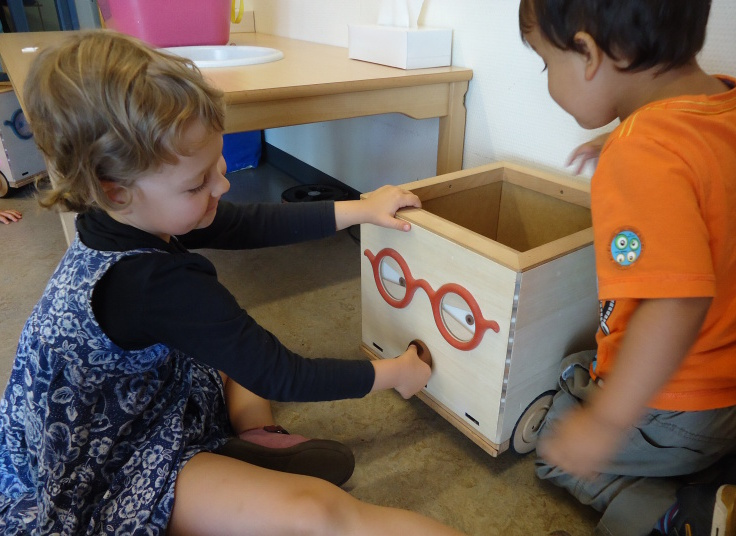
\includegraphics[height=0.2\paperheight]{ranger/croquignole-single}}
            \hspace{0.5em}
            \hyperlink{dominos}{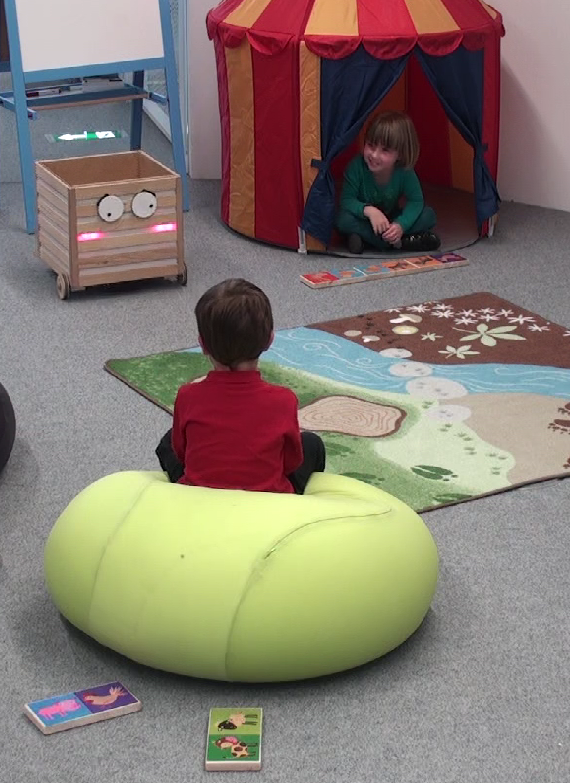
\includegraphics[height=0.2\paperheight]{ranger/domino-mistake}}
            \hspace{0.5em}
            \hyperlink{anthropomorphism}{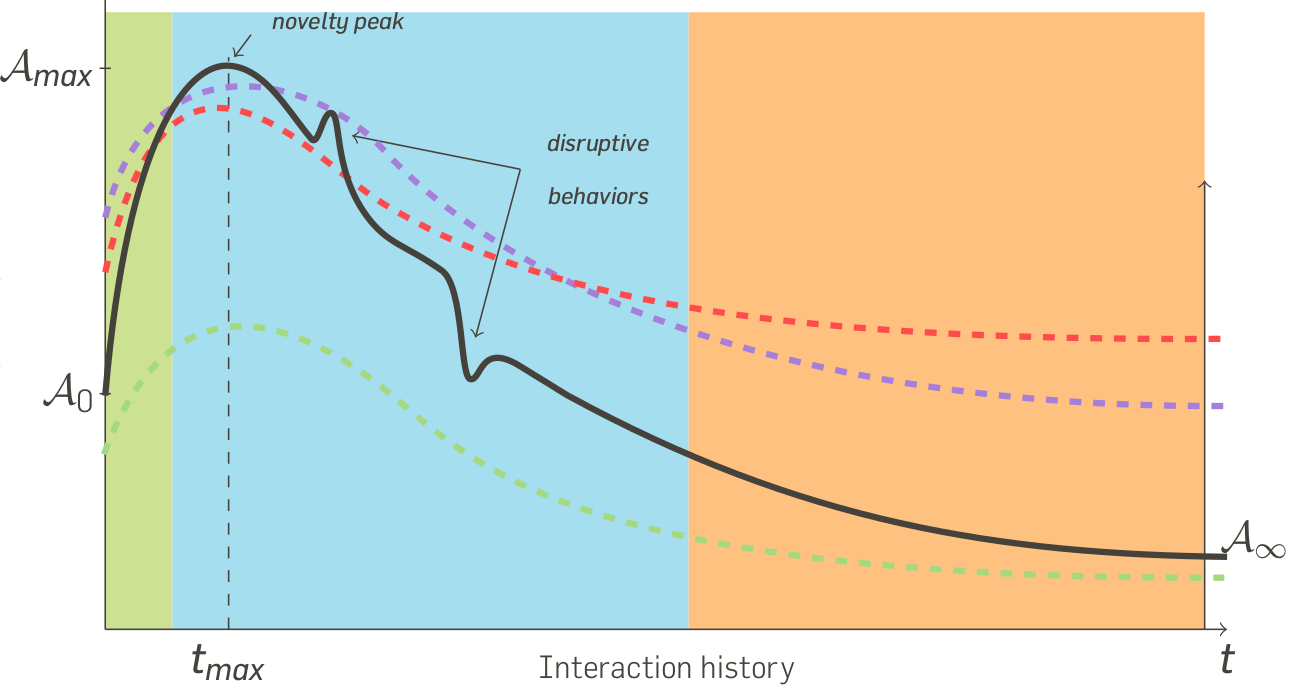
\includegraphics[height=0.2\paperheight]{dynamics_anthropo}}

        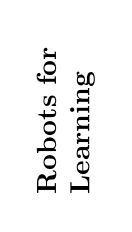
\begin{tikzpicture}
            \node[rotate=90,text width=2cm]{\textbf{Robots for \\Learning}};
        \end{tikzpicture}
            \hyperlink{cellulo}{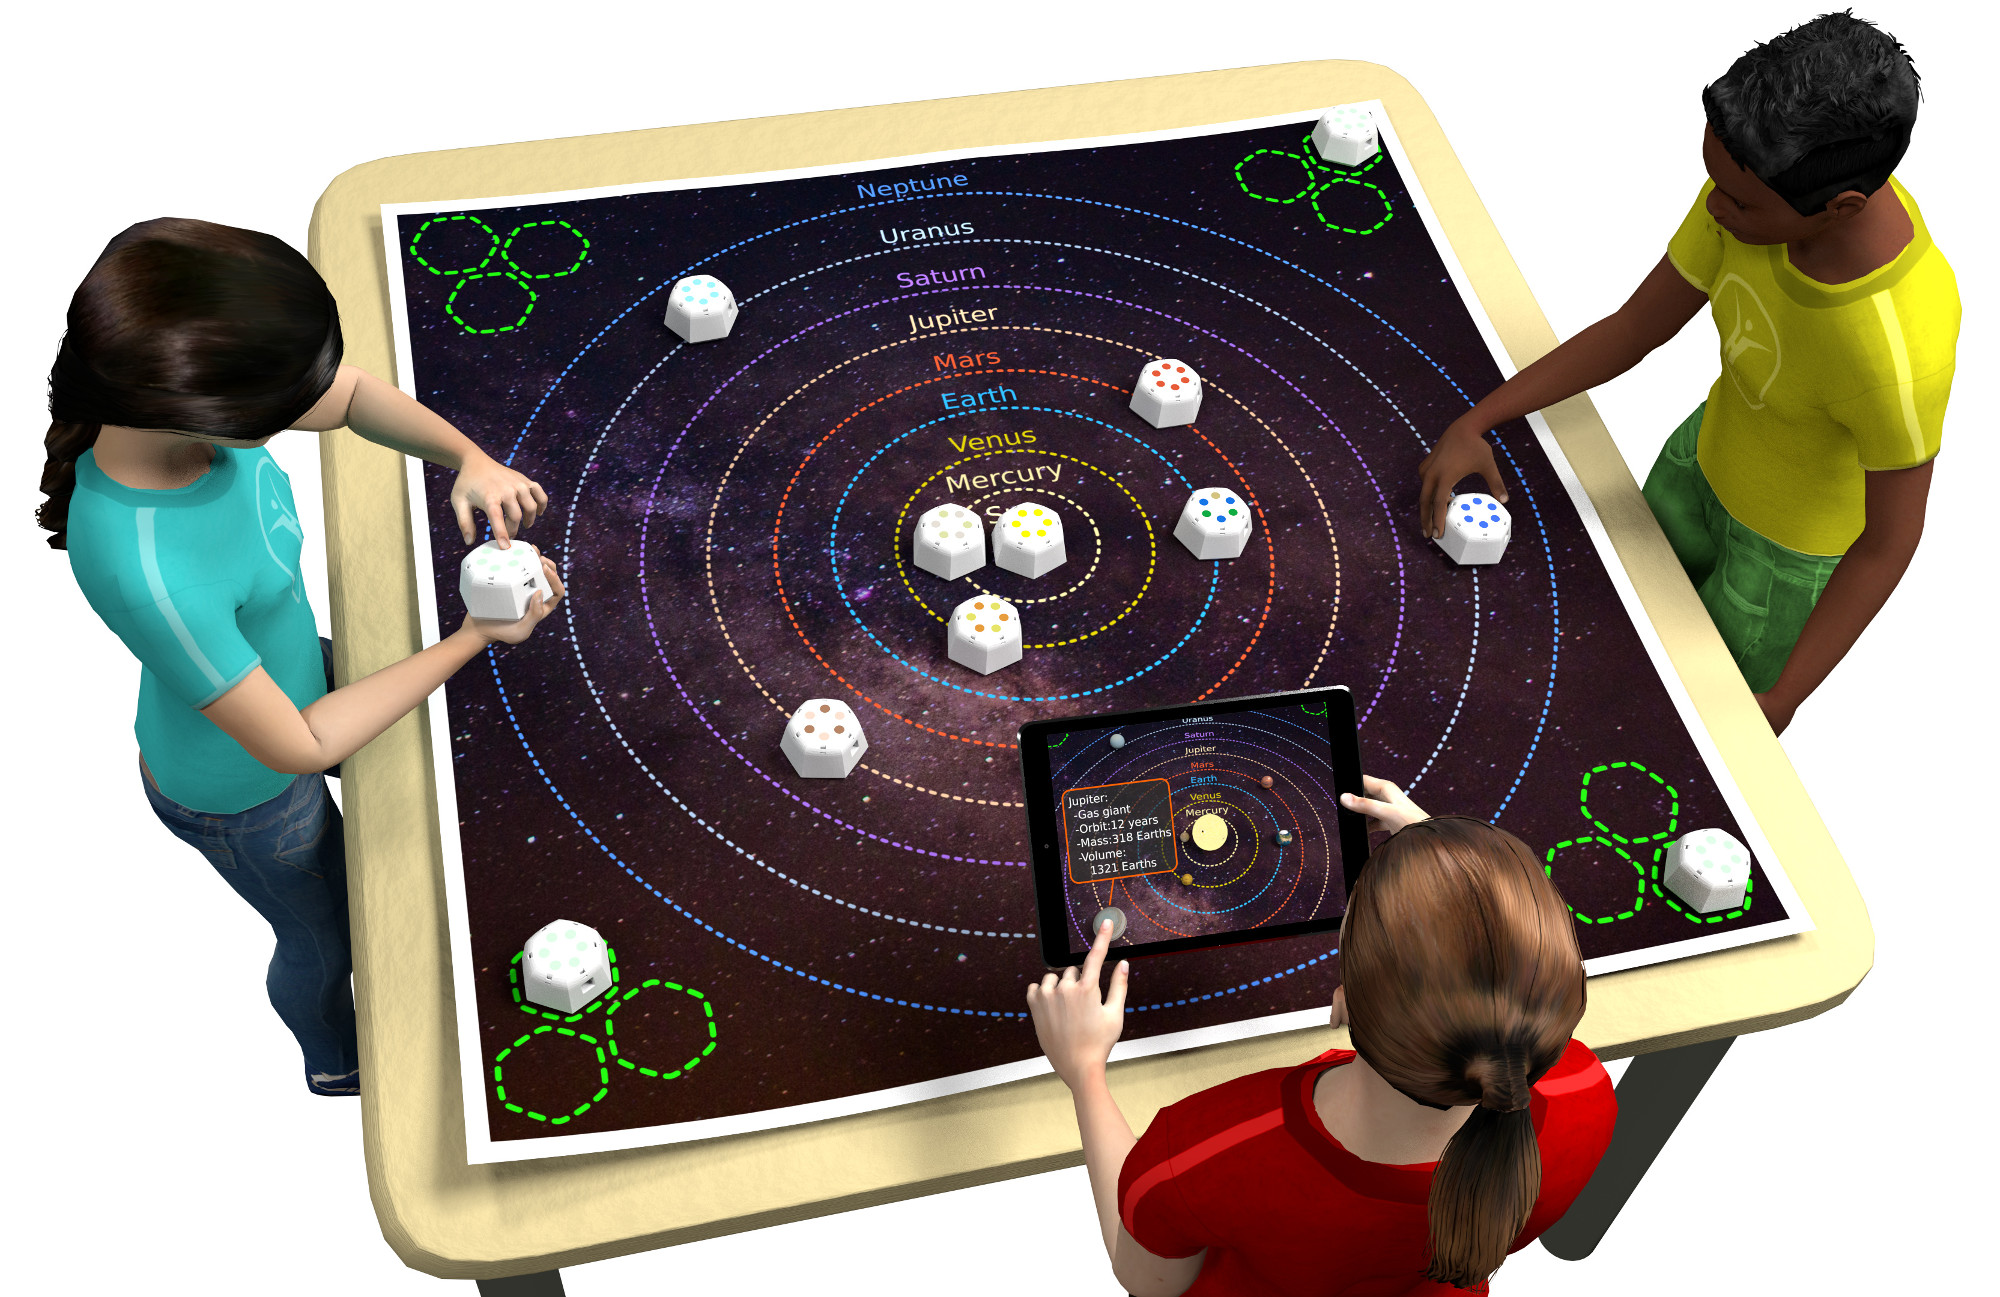
\includegraphics[height=0.2\paperheight]{cellulo/concept-solar-system}}
            \hspace{0.5em}
            \hyperlink{cowriter-impl}{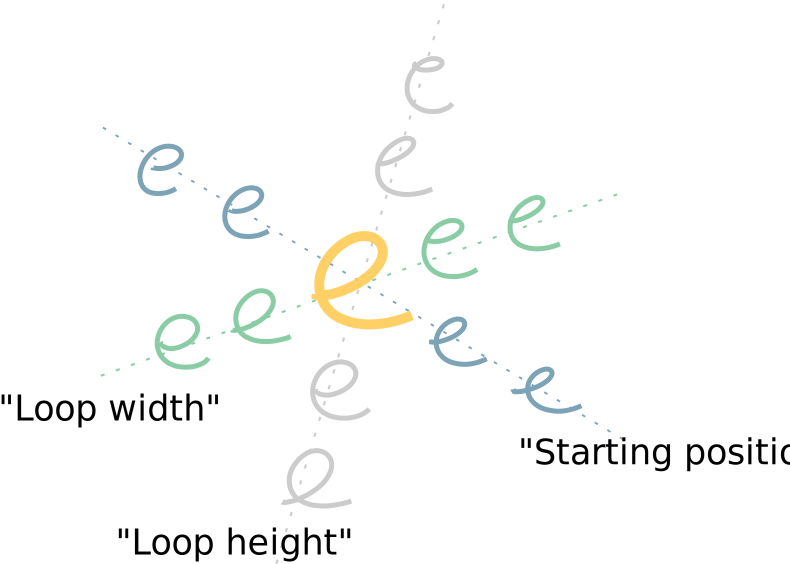
\includegraphics[height=0.2\paperheight]{cowriter/pca}}

        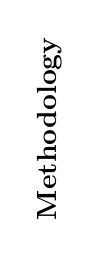
\begin{tikzpicture}
            \node[rotate=90]{\textbf{Methodology}};
        \end{tikzpicture}
            \hyperlink{withmeness}{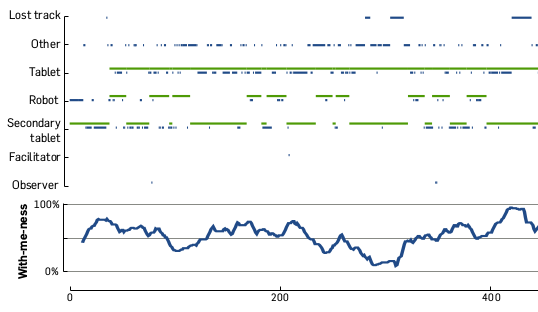
\includegraphics[height=0.2\paperheight]{withmeness/withmeness}}
            \hspace{0.5em}
            \hyperlink{asr}{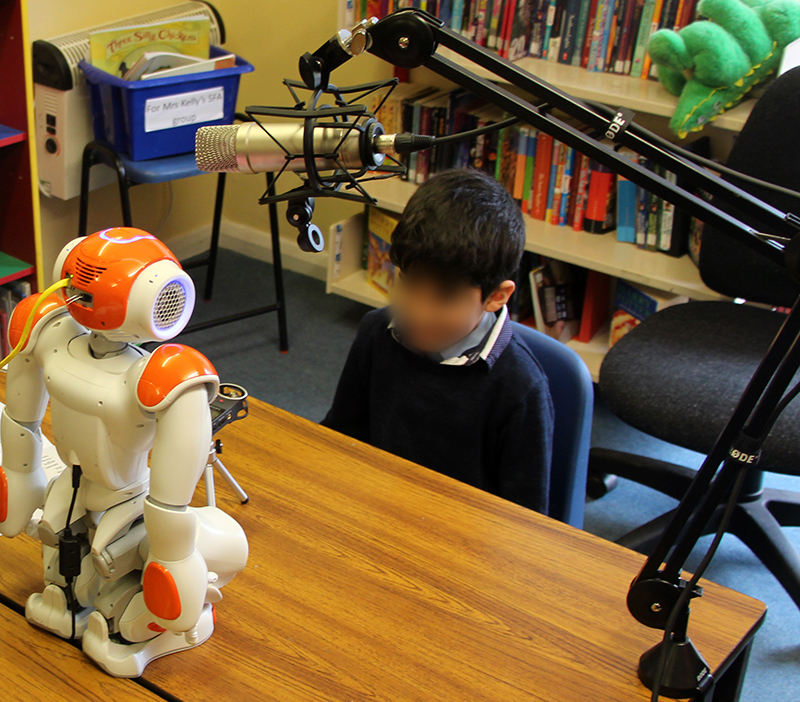
\includegraphics[height=0.2\paperheight]{speech-reco/record_img}}
            \hspace{0.5em}
            \hyperlink{constructs}{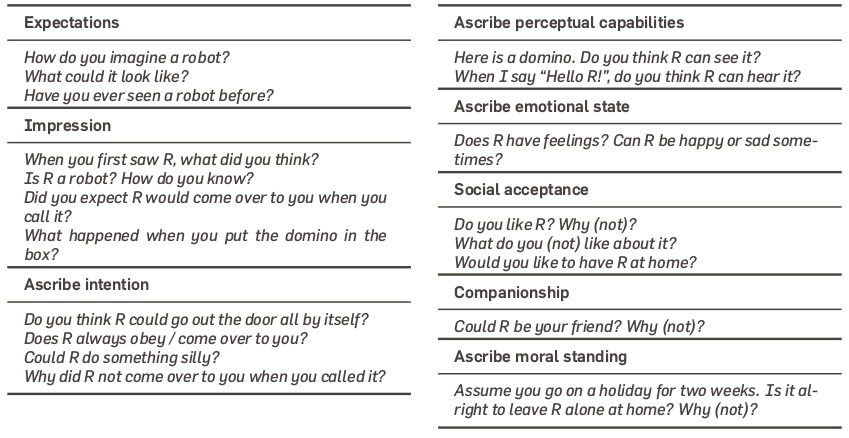
\includegraphics[height=0.2\paperheight]{ranger/questionnaire}}

\end{frame}

%%%%%%%%%%%%%%%%%%%%%%%%%%%%%%%%%%%%%%%%%%%%%%%%%%%%%%%%

\section{Future directions}

%%%%%%%%%%%%%%%%%%%%%%%%%%%%%%%%%%%%%%%%%%%%%%%%%%%%%%%%

\imageframe[color=white]{islands1}

%%%%%%%%%%%%%%%%%%%%%%%%%%%%%%%%%%%%%%%%%%%%%%%%%%%%%%%%

\imageframe[color=white]{islands2}

%%%%%%%%%%%%%%%%%%%%%%%%%%%%%%%%%%%%%%%%%%%%%%%%%%%%%%%%

\imageframe[color=white]{islands3}

%%%%%%%%%%%%%%%%%%%%%%%%%%%%%%%%%%%%%%%%%%%%%%%%%%%%%%%%

\imageframe[color=white]{islands4}
%
%{
%    \paper{Graziano {\bf Consciousness and the Social Brain} -- 2013}
%
%\begin{frame}{Towards a cognitive architecture}
%
%    Guiding research question: \textbf{What are the principles that underpin
%    social cognition?}
%
%    \pause
%
%    One working hypothesis: \textbf{Sociality emerge from interaction}
%
%    $\Rightarrow$ situated \& embodied view on social cognition
%
%    \pause
%
%    \emph{Attention Schemata} theory:
%    \begin{itemize}
%        \item \textbf{Social interaction is mediated by
%    attention}
%        \item \textbf{Modelling other's attention is building a theory of their mind}
%
%    \end{itemize}
%
%    \pause
%
%
%    Fine, but... testable predictions?
%
%    \badge{europe_plym}
%\end{frame}
%}
%%%%%%%%%%%%%%%%%%%%%%%%%%%%%%%%%%%%%%%%%%%%%%%%%%%%%%%%%
%
%\begin{frame}{Operationalising the research}
%
%    \begin{itemize}
%        \item<+-> typical socio-cognitive tasks are to simple and constrainted.
%            Do not reflect the complexity \& dynamics of real-world interactions
%        \item<+-> yet, research \emph{in the wild} is difficult to conduct
%            rigorously and to replicate
%        \item<+-> $\Rightarrow$ {\bf free play as our next horizon}: \emph{rich set of cognitive and
%            social dynamics}; importance of motivation/drive; forces us to deal
%            with uncertain and unexpected situations
%        \item<+-> But challenging as well! What is the action policy? Focus
%            instead on the \textbf{social policy}
%    \end{itemize}
%
%    \badge{europe_plym}
%\end{frame}

%%%%%%%%%%%%%%%%%%%%%%%%%%%%%%%%%%%%%%%%%%%%%%%%%%%%%%%%

\videoframe[0.56]{figs/next/maud-zoe-pilot-edit.mkv}

%%%%%%%%%%%%%%%%%%%%%%%%%%%%%%%%%%%%%%%%%%%%%%%%%%%%%%%%

%{
%    \paper{Parten, {\bf Social participation among preschool children} Journal
%    of Abnormal and Social Psychology 1932}
%\begin{frame}<5>{Theoretical framework: stages of play}
%
%    In developmental psychology, Parten's {\bf stages of play}:
%
%    \begin{enumerate}
%        \item<1-> {\bf Solitary (independent) play}: Playing separately from
%            others, with no reference to what others are doing.
%        \item<2-> {\bf Onlooker play}: Watching others play. May engage in
%            conversation but not engaged in doing. True focus on the children at
%            play.
%        \item<3-> {\bf Parallel play} (adjacent play, social coaction): Playing
%            with similar objects, clearly beside others but not with them (near
%            but not with others.)
%        \item<4-> {\bf Associative play}:  Playing with others without
%            organization of play activity. Initiating or responding to
%            interaction with peers. 
%        \item<5-> {\bf Cooperative play}: Coordinating one’s behavior with that
%            of a peer. Everyone has a role, with the emergence of a sense of
%            belonging to a group. Beginning of "team work."
%    \end{enumerate}
%
%\end{frame}
%}

%%%%%%%%%%%%%%%%%%%%%%%%%%%%%%%%%%%%%%%%%%%%%%%%%%%%%%%%

\imageframe{memory/setup}
%\videoframe[0.56]{figs/next/zoo-builder-proto-smaller.mkv}
%\imageframe[color=black]{memory/zoo+ros+memory}


%%%%%%%%%%%%%%%%%%%%%%%%%%%%%%%%%%%%%%%%%%%%%%%%%%%%%%%%

\begin{frame}{Key Predicted Social Behaviours}


    \begin{itemize}

        \item {\bf behavioural alignment}
            %: each time we play together, our
            %interaction flow improves, becomes more natural

%        \item {\bf recursive awareness}: \emph{being aware of being aware} -- typically
%            evidenced by being able to describe/verbalize its own state of
%            awareness 

        \item {\bf 'natural' (\ie emergent) turn-taking}
            %: I 'just' know when it is my
            %turn to act

        \item {\bf 'natural' protodeclarative pointing}
            %: I 'just' know when I really
            %need to draw your attention on something

        \item ability to pass non-perceptual {\bf false-belief tasks}
            %, including
            %non-perceptual, non-physical, abstract ones,

        \item {\bf replication of Parten's hierarchy}


    \end{itemize}

    \Large
    $\Rightarrow$ \textbf{scientific milestones} for human-robot interaction
\end{frame}

%%%%%%%%%%%%%%%%%%%%%%%%%%%%%%%%%%%%%%%%%%%%%%%%%%%%%%%%

\begin{frame}<2>{Research approach}

    \centering
    \begin{tikzpicture}[
         >=latex,
         every edge/.style={draw, ultra thick, <-}]

        \node (top) {\large In parallel};

        %%%%%%%%%%%%%%%%%%%%%%%%%%%%%%%%%%%%%%%%%%%%%%%%%%%%%%%%%%%%%%%%%
        \node[below left=of top] (practical) {\emph{Practical}} edge (top);
        %%%%%%%%%%%%%%%%%%%%%%%%%%%%%%%%%%%%%%%%%%%%%%%%%%%%%%%%%%%%%%%%%
        \node<1>[below=0.2 of practical,text width=5cm] (practicaldesc) {
            \begin{itemize}
                \item symbolic approach
                \item complete with respect to cognitive capabilities
                \item focus on long-term autonomy
                \item cross-hardware
            \end{itemize} };
        %%%%%%%%%%%%%%%%%%%%%%%%%%%%%%%%%%%%%%%%%%%%%%%%%%%%%%%%%%%%%%%%%
        \node<2>[below=0.2 of practical,text width=5cm] {

            \centering 

            The ``Plymouth Architecture for Socio-Cognitive Robots''

            \resizebox{\linewidth}{!}{%
            \tikzset{subpart/.style={draw, font=\scriptsize, fill opacity=0.5, text opacity=1, fill=white!50}}

            \begin{tikzpicture}[
                    >=latex,
                    every edge/.style={draw, very thick},
                    skill/.style={draw, rounded corners, align=center, inner sep=5pt, fill=black!20},
                label/.style={midway, align=center, font=\scriptsize, fill=none}]

                %%% Separation between deliberative layer and sensori-motor layer
                \draw[dotted, thick] (-8,-5) -- (12, -5);

                %%% SPARK
                    \node at (3,-3.5)[skill, fill=hriSec3!50] (spark) {%
                        Geometric \& Temporal Reasoning
                };

                %%% LOWLEVEL
                \node [skill, below=0.7 of spark,fill=gray!50] (lowlevel) {%
                        Sensorimotor layer;
                };

                \path (lowlevel) edge [->] (spark);

                %%% ORO
                \node at (0,0)[skill, ultra thick, fill=hriSec2Dark!50] (oro)
                {Symbolic facts \\ and beliefs management};
                \path (spark.100) edge [->, bend right] node[label] {symbolic \\ facts} (oro);

                %%% HATP
                \node at (-6, 2.5)[skill, fill=hriSec1!50] (hatp) {Human-aware
                symbolic \\task planning};
                \path (hatp) edge [<->, bend right] node[label] {world model and \\ agents beliefs} (oro.170);

                %%% DIALOGS
                \node at (-6, -3) [skill, fill=hriSec3Dark!50] (dialogs)
                {Dialogue processing};
                \path (dialogs) edge [<->, bend left] node[label] {natural language \\ grounding} (oro.190);
                %%% SHARY
                \node at (3,4.5)[skill, fill=hriSec1Comp!50] (shary) {%
                    \begin{tikzpicture}
                        \node at (0,0) (exec) {Execution Controller};
                    \end{tikzpicture}
                };
                \path (shary) edge [<->, bend left] node[label] {events, \\ world model and \\ agents beliefs} (oro);
                \path (shary) edge [<->, bend left, looseness=0.8] node[label] {action monitoring \\ and management of \\ position hypotheses} (spark);
                \path (shary.west) edge [<->, bend right] node[label] {shared \\ plans} (hatp);
                %%% MHP
                \node at (8,0)[skill, fill=hriSec3CompDark!50] (mhp) {Human-aware Motion \\ and Manipulation Planning};
                \path (shary.340) edge [<->, bend left] node[label] {motion plan \\ requests} (mhp);
                \path (spark.5) edge [->, bend right] node[label] {environment\\model} (mhp);
                \path (lowlevel.east) edge [<-, bend right=60, looseness=1.2] node[label] {atomic\\actions} (mhp.south east);

            \end{tikzpicture}
            }


        };




        %%%%%%%%%%%%%%%%%%%%%%%%%%%%%%%%%%%%%%%%%%%%%%%%%%%%%%%%%%%%%%%%%
        %%%%%%%%%%%%%%%%%%%%%%%%%%%%%%%%%%%%%%%%%%%%%%%%%%%%%%%%%%%%%%%%%
        \node[below right=of top] (basic) {\emph{Basic research}} edge (top);
        %%%%%%%%%%%%%%%%%%%%%%%%%%%%%%%%%%%%%%%%%%%%%%%%%%%%%%%%%%%%%%%%%
        \node<1>[below=0.2 of basic, text width=7cm] (basicdesc) {
            \begin{itemize}
                \item principled approach
                \item emergent paradigm
                \item initially based on the \emph{attention schemata theory}
                \item associative memory networks
            \end{itemize}
        };
        \node<2>[below=0.2 of basic, text width=5cm] {
            \centering 

            Emergent Social Cognition

            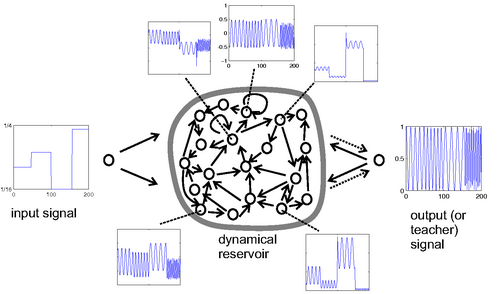
\includegraphics[width=\linewidth]{memory/echostate}

            $\rightarrow$ RNNs; \textbf{deep learning}


        };

        \only<1>{
        \coordinate (bottom) at (top |- practicaldesc.south);
        \node<1>[below=1 of bottom] (hyb) {cross-pollination};
        \draw<1>[<->,thick] (practicaldesc.south) to[bend right] (basicdesc.south);
    }


    \end{tikzpicture}


\end{frame}


%%%%%%%%%%%%%%%%%%%%%%%%%%%%%%%%%%%%%%%%%%%%%%%%%%%%%%%%

\begin{frame}{Scaffolding the research}

            \begin{center}
                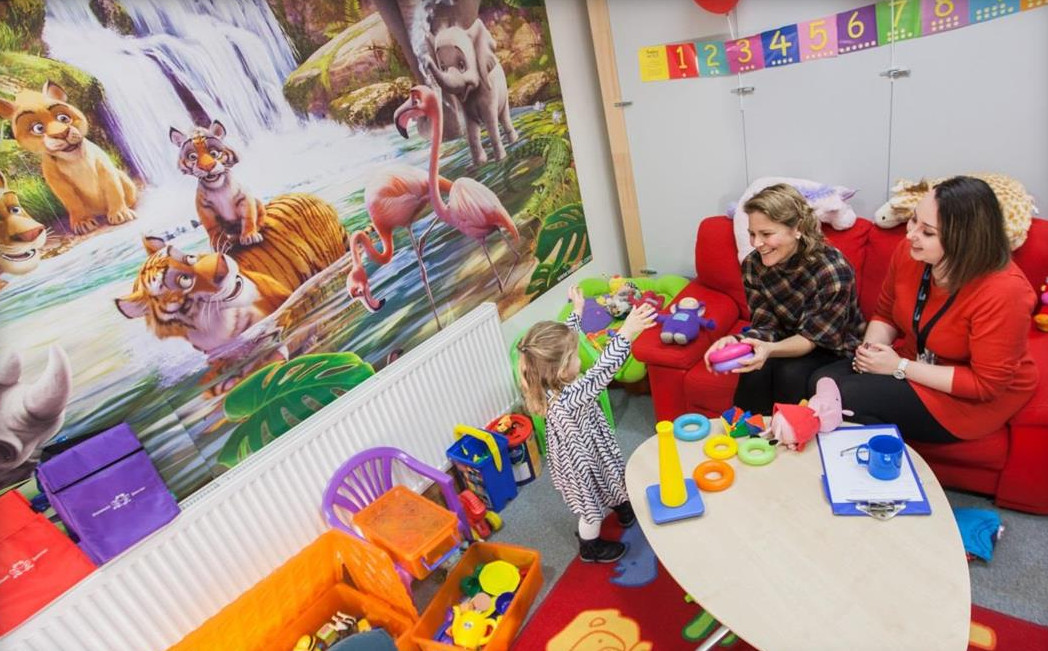
\includegraphics[width=0.6\linewidth]{plymouth/babylab}

            \end{center}

            Build up Plymouth's \textbf{KidsLab}
                \begin{itemize}
                    \item experimental space suited for 5 to 13 years old
                    \item fully equipped (recording, tracking, touch tables)
                    \item in close cooperation with Caroline Floccia \& the
                        BabyLab
                \end{itemize}

\end{frame}

%%%%%%%%%%%%%%%%%%%%%%%%%%%%%%%%%%%%%%%%%%%%%%%%%%%%%%%%

\begin{frame}{Funding}

    \only<1>{
    Short term

    \begin{itemize}
        \item {\bf EPSRC First Grant}
            \begin{itemize}
                \item up to \pounds 125,000
                \item funding for the \textbf{KidsLab} project
                \item equipment + one post-doc
            \end{itemize}
        \item {\bf EPSRC Early Career Fellowship}
            \begin{itemize}
                \item max 5 years
                \item focus on {\bf Emergence of artificial social cognition}
                \item possible partnerships: developmental robotics
                    (\eg INRIA Flowers), cognitive neurosciences (\eg Graziano
                    lab), learning technologies (\eg EPFL CHILI Lab)
            \end{itemize}
    \end{itemize}
    }
    \only<2>{
    Within 2-3 years

    \begin{itemize}
        \item {\bf Co-Investigator on a H2020 project}
            \begin{itemize}
                \item close contacts with IST Lisbon, LAAS-CNRS, EPFL,
                    INRIA Bordeaux
            \end{itemize}
        \item Submit a {\bf EPSRC Standard Research} proposal
            \begin{itemize}
                \item reaching independence
                \item focus on socio-cognitive architecture + long-term field deployment
                \item multi-proposal submission, possibly with
                    Lincoln U. (expertise on Cognitive Architectures)
            \end{itemize}
        \item {\bf ERC Starting Grant}
            \begin{itemize}
                \item up to \EUR 1.5m
                \item within 7 years of PhD completion, \ie before 2019
                \item project on {\bf Emergence of artificial social cognition}
            \end{itemize}
    \end{itemize}
    }

\end{frame}

%%%%%%%%%%%%%%%%%%%%%%%%%%%%%%%%%%%%%%%%%%%%%%%%%%%%%%%%

{
    \fullbackground[color=black]{eeg-headset}
\begin{frame}[plain]

    \vspace{8cm}

\setbeamercolor{hriSec1Demo}{fg=white!70!black}
\begin{beamercolorbox}[wd=\linewidth,ht=6ex,dp=0.7ex]{hriSec1Demo}
    \textbf{Thank you!}\\
    \scriptsize
    Séverin Lemaignan\\
    {\tt severin.lemaignan@plymouth.ac.uk}
\end{beamercolorbox}
    \vfill
\end{frame}
}

%%%%%%%%%%%%%%%%%%%%%%%%%%%%%%%%%%%%%%%%%%%%%%%%%%%%%%%%

\appendix
\begin{frame}[label=appendix]{Supplementary material}
    \small
    \begin{multicols}{2}
    \tableofcontents[hideallsubsections]
    %\tableofcontents
    \end{multicols}
\end{frame}
%%%%%%%%%%%%%%%%%%%%%%%%%%%%%%%%%%%%%%%%%%%%%%%%%%%%%%%%

\section{Performing in Human Environments}

%%%%%%%%%%%%%%%%%%%%%%%%%%%%%%%%%%%%%%%%%%%%%%%%%%%%%%%%

\videoframe[0.7]{figs/cleantable/clean-table.webm}

%%%%%%%%%%%%%%%%%%%%%%%%%%%%%%%%%%%%%%%%%%%%%%%%%%%%%%%%

{
    \paper{Lemaignan et al., {\bf Artificial Cognition for Social Human-Robot
    Interaction: An Implementation}, Artifical Intelligence, 2016}
\begin{frame}{``Cleaning the table''...}
\centering
\resizebox{!}{0.75\paperheight}{%
\begin{tikzpicture}[
        >=latex,
        every edge/.style={draw, ultra thick, ->},
        every node/.style={align=center},
        robot/.style={fill=hriSec2Comp!50},
        plan/.style={draw,
                     thick,  
                     circle, 
                     font=\sf,
                     align=center,
                     fill=hriSec3CompDark!50, 
                     minimum size=1cm, 
                     inner sep=0.1cm}
        ]

        \coordinate<1> (figbottom) at (-0.5, -28.5);
        \coordinate<2-5> (figbottom) at (-0.5, -10.5);
        \node<2-5> at (0,5) {};
        \node<2-5> at ($(figbottom) + (0,-5)$) {};


        \fill[gray!10!white] (4.6,.5) rectangle (figbottom);

        \path (-0.5,0) edge (figbottom) node[sloped, above left, rotate=90] {\large\bf time};

        \node at (2,0) (percept) {\bf Perception};
            \node[below=0.5 of percept.south west, anchor=mid] {camera};
            \node[below=0.5 of percept.south east, anchor=mid] {3D model};

        \node[right=4 of percept, minimum width=2.5cm] (kb) {\bf Knowledge};
            \node[below=0.5 of kb.south west, anchor=mid east] (kbr) {robot};
            \node[below=0.5 of kb.south east, anchor=mid west] (kbh) {human};
            \draw[dotted] (kbr) to (figbottom -| kbr);
            \draw[dotted] (kbh) to (figbottom -| kbh);

        \fill[gray!10!white] (12,.5) rectangle (17,0 |- figbottom);
        \node[right=4.5 of kb] (plan) {\bf Plan};
            \node[below=0.5 of plan.south west, anchor=mid east] (probot) {robot};
            \node[below=0.5 of plan.south east, anchor=mid west] (phuman) {human};
            \draw[dotted] (probot) to (figbottom -| probot);
            \draw[dotted] (phuman) to (figbottom -| phuman);

        \node[right=5 of plan] (action) {\bf Actions};
            \node[below=0.5 of action.south west, anchor=mid east] (arobot) {robot};
            \node[below=0.5 of action.south east, anchor=west] (ahuman) {human\\(monitoring)};
            \draw[dotted] (arobot) to (figbottom -| arobot);
            \draw[dotted] (ahuman) to (figbottom -| ahuman);

        \draw[dashed] (-0.6,-1.2) --(24, -1.2);

        \node<1,2>[anchor=east] at (-0.5, -3) (t1) {\Large $t_1$};
        \node<1,2>[anchor=east, below=6 of t1] (t2) {\Large $t_2$};
        \node<3>[anchor=east] at (-0.5, -3) (t2) {\Large $t_2$};
        \node<1,3>[anchor=east, below=6 of t2] (t3) {\Large $t_3$};
        \node<4>[anchor=east] at (-0.5, -3) (t3) {\Large $t_3$};
        \node<1,4>[anchor=east, below=4 of t3] (t4) {\Large $t_4$};
        \node<5>[anchor=east] at (-0.5, -3) (t4) {\Large $t_4$};
        \node<1,5>[anchor=east, below=5 of t4] (t5) {\Large $t_5$};

        %%%%%%%%%%%%%%%%%%%%%%%%%%%%%%%%%%%%%%%%%%%%%%%%%%%%%%%%%%%%%%%%%%%%%%%%%%%%%%%%%%%%%%%%%%%%
        %%% PERCEPTIONS
        %%%%%%%%%%%%%%%%%%%%%%%%%%%%%%%%%%%%%%%%%%%%%%%%%%%%%%%%%%%%%%%%%%%%%%%%%%%%%%%%%%%%%%%%%%%%

        \node<1,2> at (t1 -| percept) (cam1) {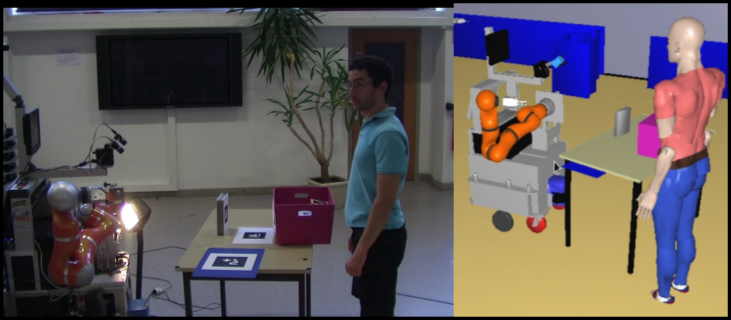
\includegraphics[height=2cm]{cleantable/manip_run_cam1.png}};
        \node<1,3> at (t2 -| percept) (cam2) {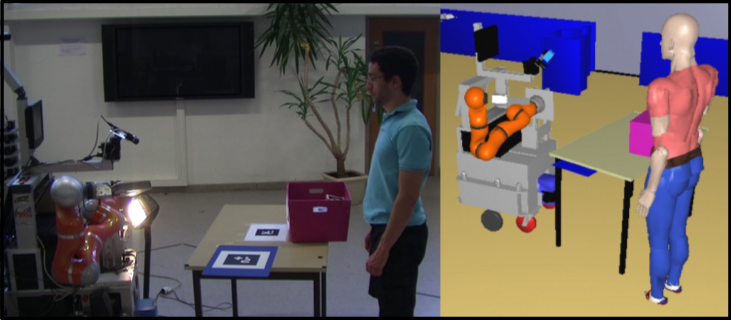
\includegraphics[height=2cm]{cleantable/manip_run_cam2.png}};
        \node<1,4> at (t3 -| percept) (cam3) {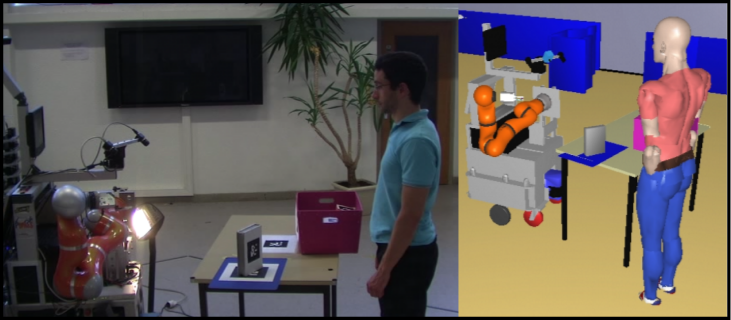
\includegraphics[height=2cm]{cleantable/manip_run_cam3.png}};
        \node<1,5> at (t4 -| percept) (cam4) {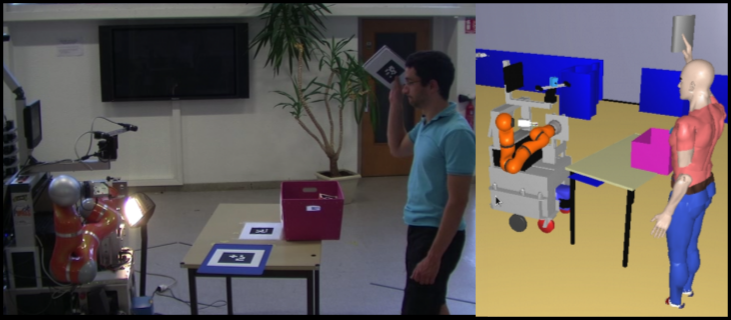
\includegraphics[height=2cm]{cleantable/manip_run_cam4.png}};
        \node<1,5> at (t5 -| percept) (cam5) {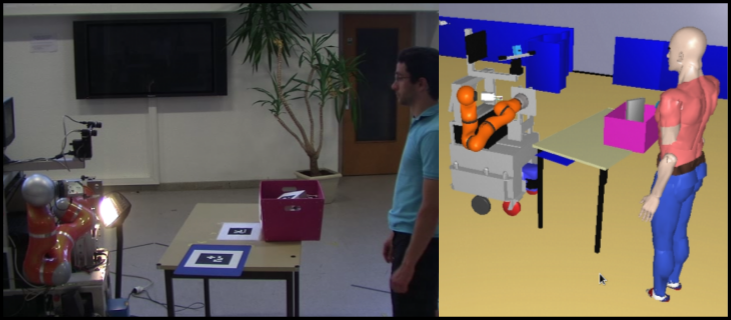
\includegraphics[height=2cm]{cleantable/manip_run_cam5.png}};

        %%%%%%%%%%%%%%%%%%%%%%%%%%%%%%%%%%%%%%%%%%%%%%%%%%%%%%%%%%%%%%%%%%%%%%%%%%%%%%%%%%%%%%%%%%%%
        %%% KNOWLEDGE
        %%%%%%%%%%%%%%%%%%%%%%%%%%%%%%%%%%%%%%%%%%%%%%%%%%%%%%%%%%%%%%%%%%%%%%%%%%%%%%%%%%%%%%%%%%%%

        \node<1,2>[fill=white,align=left] at (cam1 -| kbr) (kb1) {\stmt{TAPE isVisible true}\\
                                                        \stmt{TAPE isReachable true}\\
                                                        \stmt{TAPE isOn TABLE}\\
                                                        \stmt{BIN isVisible true}\\
                                                        \stmt{BIN isReachable false}};

        \node<1,2>[fill=white,align=left] at (cam1 -| kbh) {\stmt{TAPE isVisible true}\\
                                                        \stmt{TAPE isReachable false}\\
                                                        \stmt{TAPE isOn TABLE}\\
                                                        \stmt{BIN isVisible true}\\
                                                        \stmt{BIN isReachable true}};

        \node<1,3>[fill=white,align=left] at (cam2 -| kbr) (kb2) {\stmt{ROBOT hasInHand TAPE}};


        \node<1,4>[fill=white,align=left] at (cam3 -| kbr) {\stmt{TAPE isReachable true}\\
                                            \stmt{TAPE isVisible true} \\
                                            \stmt{TAPE isOn TABLE}};

        \node<1,4>[fill=white,align=left ] at (cam3 -| kbh) (kb3) {\stmt{TAPE isReachable true}\\
                                             \stmt{TAPE isVisible true}};

        \node<1,5>[fill=white,align=left] at (cam4 -| kbh) (kb4) {\stmt{HUMAN hasInHand TAPE}};

        \node<1,5>[fill=white,align=left] at (cam5 -| kbr)  {\stmt{TAPE isIn BIN}};
        \node<1,5>[fill=white,align=left] at (cam5 -| kbh) (kb5) {\stmt{TAPE isIn BIN}};

        %%%%%%%%%%%%%%%% %%%%%%%%%%%%%%%%%%%%%%%%%%%%%%%%%%%%%%%%%%%%%%%%%%%%%%%%%%%%%%%%%%%%%%%%%%%%
        %%% PLANS
        %%%%%%%%%%%%%%%%%%%%%%%%%%%%%%%%%%%%%%%%%%%%%%%%%%%%%%%%%%%%%%%%%%%%%%%%%%%%%%%%%%%%%%%%%%%%

        \node<1,2>[fill=gray!10!white,below=1 of plan] (incoming) {\bf \Large Incoming goal \\ \it Clean the table!};

        \node<1,2>[anchor=north, plan, robot] at (cam1.south -| probot) (pr1) {\bf TAKE\\TAPE\\TABLE};
        \node<1,3>[anchor=north, plan, robot] at (cam2.south -| probot)  (pr2) {\bf PUTRV\\TAPE\\TABLE} edge[<-] (pr1);
        \node<1,4>[anchor=north, plan] at (cam3.south -| phuman) (ph1) {\bf TAKE\\TAPE\\TABLE} edge[<-] (pr2);
        \node<1,5>[anchor=north, plan]  at (cam4.south -| phuman) (ph2) {\bf PUT\\TAPE\\BIN} edge[<-] (ph1);

        \node<1,5>[fill=gray!10!white,anchor=north] at (cam5.south -| plan) (done) {\bf \Large Goal completed};

        %%%%%%%%%%%%%%%%%%%%%%%%%%%%%%%%%%%%%%%%%%%%%%%%%%%%%%%%%%%%%%%%%%%%%%%%%%%%%%%%%%%%%%%%%%%%
        %%% ACTIONS
        %%%%%%%%%%%%%%%%%%%%%%%%%%%%%%%%%%%%%%%%%%%%%%%%%%%%%%%%%%%%%%%%%%%%%%%%%%%%%%%%%%%%%%%%%%%%

        \only<1,2>{
        \node[fill=white] at (pr1 -| arobot) (ep1) {\it evaluate pre-conditions};

        \node[below=0.1 of ep1] (mhp1) {%
            \begin{tikzpicture}
                \node[fill=white] (title) {\bf motion planning};
                \node[below=0.1 of title.south west, label=below:{\tt PICK\_GOTO}] (mapg) {
\includegraphics{cleantable/MHP_ARM_PICK_GOTO}};
                \node[fill=white,right=of mapg, label=below:{\tt TAKE\_TO\_FREE}] (mattf) {\includegraphics{cleantable/MHP_ARM_TAKE_TO_FREE}} edge[<-] (mapg);
            \end{tikzpicture}
        };
        \node[fill=white,below=0.1 of mhp1] (me1) {\bf motion execution};
        \node[fill=white,below=0.1 of me1] (ae1) {\it assess post-conditions};
        }
        %%%%%%%%%%%%%%%%%%%%%%%%%%%%%%%%%%%%%%%%%%%%%%%%%%%%%%%%%%%%%%%%%%%%%%%%%%%%%%%%%%%%%%%%%%%%%
        \only<1,3>{
        \node[fill=white] at (pr2 -| arobot) (ep2) {\it evaluate pre-conditions};

        \node[below=0.1 of ep2] (mhp2) {%
            \begin{tikzpicture}
                \node[fill=white] (title) {\bf motion planning};
                \node[fill=white,below=0.1 of title, label=below:{\tt ESCAPE}] (maeo) {\includegraphics{cleantable/MHP_ARM_ESCAPE_OBJECT}};
                \node[left=of maeo, label=below:{\tt PLACE\_FROM\_FREE}] (mapff) {\includegraphics{cleantable/MHP_ARM_PLACE_FROM_FREE}} edge (maeo);
                \node[fill=white,right=of maeo, label=below:{\tt TO\_FREE}] (maf) {\includegraphics{cleantable/MHP_ARM_FREE}} edge[<-] (maeo);
            \end{tikzpicture}
        };
        \node[fill=white,below=0.1 of mhp2] (me2) {\bf motion execution};
        \node[fill=white,below=0.1 of me2] (ae2) {\it assess post-conditions};
        }
        %%%%%%%%%%%%%%%%%%%%%%%%%%%%%%%%%%%%%%%%%%%%%%%%%%%%%%%%%%%%%%%%%%%%%%%%%%%%%%%%%%%%%%%%%%%%%

        \node<1,4>[anchor=north] at (ph1 -| ahuman) (wait1) {%
            \begin{tikzpicture}
                \node[fill=white] (title) {\it wait for pick\\ {\tt TAPE} \it from {\tt TABLE}};
                \node[below=0.1 of title] {\includegraphics{cleantable/wait_for_pick}};
            \end{tikzpicture}
        };

        \node<1,5>[anchor=north] at (ph2 -| ahuman) (wait2) {%
            \begin{tikzpicture}
                \node[fill=white] (title) {\it wait for put\\ {\tt TAPE} \it into {\tt BIN}};
                \node[below=0.1 of title] {\includegraphics{cleantable/wait_for_throw}};
            \end{tikzpicture}
        };


        %%%%%%%%%%%%%%%%%%%%%%%%%%%%%%%%%%%%%%%%%%%%%%%%%%%%%%%%%%%%%%%%%%%%%%%%%%%%%%%%%%%%%%%%%%%%
        %%% FLOW
        %%%%%%%%%%%%%%%%%%%%%%%%%%%%%%%%%%%%%%%%%%%%%%%%%%%%%%%%%%%%%%%%%%%%%%%%%%%%%%%%%%%%%%%%%%%%
        \draw<1,2>[dotted, ->, in=45, out=180] (incoming.west) to (kb1);
        \draw<1,2>[dotted, ->, bend right] (kb1) to (pr1);
        \draw<1,2>[dotted, ->, bend left] (pr1) to (ep1);
        \draw<1,2>[dotted, ->, in=45, out=180] (ae1.west) to (kb2);
        \draw<1,3>[dotted, ->, bend right] (kb2) to (pr2);
        \draw<1,3>[dotted, ->, bend left] (pr2) to (ep2);
        \draw<1>[dotted, ->, in=45, out=180] (ae2.west) to (kb3);
        \draw<1,4>[dotted, ->, bend right] (kb3) to (ph1);
        \draw<1,4>[dotted, ->, bend left] (ph1) to (wait1);
        \draw<1>[dotted, ->, in=-20, out=180] (wait1.west) to (kb4.east);
        \draw<1,5>[dotted, ->, bend right] (kb4) to (ph2);
        \draw<1,5>[dotted, ->, bend left] (ph2) to (wait2);
        \draw<1,5>[dotted, ->, in=20, out=180] (wait2.west) to (kb5);
        \draw<1,5>[dotted, ->, bend left] (kb5.east) to (done.north);


 \end{tikzpicture}
 }
\end{frame}
}

%%%%%%%%%%%%%%%%%%%%%%%%%%%%%%%%%%%%%%%%%%%%%%%%%%%%%%%%

\begin{frame}{Planning for the Human}

    \begin{figure}
        \centering

        \resizebox{0.7\paperwidth}{!}{%
            \begin{tikzpicture}[
                    >=latex,
                    robot/.style={fill=hriSec1CompDark!50},
                    every edge/.style={<-, draw, ultra thick},
                    every node/.style={ draw, 
                        thick,  
                        circle, 
                        font=\sf,
                        align=center,
                        node distance=2cm,
                        fill=hriSec3CompDark!50, 
                        minimum size=2cm, 
                inner sep=0.1cm}]

                \node[font=\large, draw=none, fill=none, rotate=90] at (-2, 0) {Human\\actions};
                \node[font=\large, draw=none, fill=none, rotate=90] at (-2, -3.5) {Robot\\actions};

                \node (h1) {\hatpaction{TAKE}{GREY\_TAPE}{TABLE}};
                \node[right=of h1] (h2) {\hatpaction{PUT}{GREY\_TAPE}{BIN1 }} edge (h1);

                \node[robot, below=1.5 of h1] (r1) {\hatpaction{TAKE}{BLACK\_TAPE}{TABLE }};
                \node[robot, right=of r1] (r2) {\hatpaction{PUT}{BLACK\_TAPE}{BIN2 }} edge (r1);
                \node[robot, right=of r2] (r3) {\hatpaction{TAKE}{BOTTLE}{TABLE }} edge (r2);
                \node[robot, right=of r3] (r4) {\hatpaction{PUTRV}{BOTTLE}{TABLE}} edge (r3);
                \node[robot, right=of r4] (r5) {\hatpaction{TAKE}{BOOK}{TABLE }} edge (r4);
                \node[robot, right=of r5] (r6) {\hatpaction{PUT}{BOOK}{BIN2 }} edge (r5);

                \node at (r5 |- h1) (h3) {\hatpaction{TAKE}{BOTTLE}{TABLE}} edge (h2) edge (r4);
                \node[right=of h3] (h4) {\hatpaction{PUT}{BOTTLE}{BIN1}} edge (h3);

            \end{tikzpicture}
        }

        \vspace*{1cm}

        \onslide<2>
        \resizebox{0.7\paperwidth}{!}{%
            \begin{tikzpicture}[
                    >=latex,
                    robot/.style={fill=hriSec1CompDark!50},
                    every edge/.style={<-, draw, ultra thick},
                    every node/.style={ draw, 
                        thick,  
                        circle, 
                        font=\sf,
                        align=center,
                        node distance=2cm,
                        fill=hriSec3CompDark!50, 
                        minimum size=2cm, 
                inner sep=0.1cm}]

                \node[font=\large, draw=none, fill=none, rotate=90] at (-2, 0) {Human\\actions};
                \node[font=\large, draw=none, fill=none, rotate=90] at (-2, -3.5) {Robot\\actions};


                \node (h1) {\hatpaction{TAKE}{GREY\_TAPE}{TABLE}};
                \node[right=of h1] (h2) {\hatpaction{PUT}{GREY\_TAPE}{BIN1 }} edge (h1);

                \node[robot, below=1.5 of h1] (r3) {\hatpaction{TAKE}{BOTTLE}{TABLE }};
                \node[robot, right=of r3] (r4) {\hatpaction{PUTRV}{BOTTLE}{TABLE}} edge (r3);
                \node[robot, right=of r4] (r1) {\hatpaction{TAKE}{BLACK\_TAPE}{TABLE }} edge (r4);
                \node[robot, right=of r1] (r2) {\hatpaction{PUT}{BLACK\_TAPE}{BIN2 }} edge (r1);
                \node[robot, right=of r2] (r5) {\hatpaction{TAKE}{BOOK}{TABLE }} edge (r2);
                \node[robot, right=of r5] (r6) {\hatpaction{PUT}{BOOK}{BIN2 }} edge (r5);

                \node[right=of h2] (h3) {\hatpaction{TAKE}{BOTTLE}{TABLE}} edge (h2) edge (r4);
                \node[right=of h3] (h4) {\hatpaction{PUT}{BOTTLE}{BIN1}} edge (h3);

            \end{tikzpicture}
        }

    \end{figure}
\end{frame}

%%%%%%%%%%%%%%%%%%%%%%%%%%%%%%%%%%%%%%%%%%%%%%%%%%%%%%%%

\begin{frame}{Planning for the Human}

    \begin{figure}
        \centering
        \includegraphics[width=0.6\textwidth]{cleantable.jpg}\\

        \vspace*{1em}

        \resizebox{0.7\paperwidth}{!}{%
            \begin{tikzpicture}[
                    >=latex,
                    robot/.style={fill=hriSec1CompDark!50},
                    every edge/.style={<-, draw, ultra thick},
                    every node/.style={ draw, 
                        thick,  
                        circle, 
                        font=\sf,
                        align=center,
                        node distance=2cm,
                        fill=hriSec3CompDark!50, 
                        minimum size=2cm, 
                inner sep=0.1cm}]

                \node[font=\large, draw=none, fill=none, rotate=90] at (-2, 0) {Human\\actions};
                \node[font=\large, draw=none, fill=none, rotate=90] at (-2, -3.5) {Robot\\actions};

                \node (h1) {\hatpaction{TAKE}{GREY\_TAPE}{TABLE}};
                \node[right=of h1] (h2) {\hatpaction{PUT}{GREY\_TAPE}{BIN1 }} edge (h1);

                \node[robot, below=1.5 of h1] (r1) {\hatpaction{TAKE}{BLACK\_TAPE}{TABLE }};
                \node[robot, right=of r1] (r2) {\hatpaction{PUT}{BLACK\_TAPE}{BIN2 }} edge (r1);
                \node[robot, right=of r2] (r3) {\hatpaction{TAKE}{BOTTLE}{TABLE }} edge (r2);
                \node[robot, right=of r3] (r4) {\hatpaction{PUTRV}{BOTTLE}{TABLE}} edge (r3);
                \node[robot, right=of r4] (r5) {\hatpaction{TAKE}{BOOK}{TABLE }} edge (r4);
                \node[robot, right=of r5] (r6) {\hatpaction{PUT}{BOOK}{BIN2 }} edge (r5);

                \node at (r5 |- h1) (h3) {\hatpaction{TAKE}{BOTTLE}{TABLE}} edge (h2) edge (r4);
                \node[right=of h3] (h4) {\hatpaction{PUT}{BOTTLE}{BIN1}} edge (h3);

            \end{tikzpicture}
        }

    \end{figure}

\end{frame}

%%%%%%%%%%%%%%%%%%%%%%%%%%%%%%%%%%%%%%%%%%%%%%%%%%%%%%%%

\videoframe[0.56]{videos/variations-splitscreen.mpg}

%%%%%%%%%%%%%%%%%%%%%%%%%%%%%%%%%%%%%%%%%%%%%%%%%%%%%%%%

\videoframe{videos/roboscopie.webm}

%%%%%%%%%%%%%%%%%%%%%%%%%%%%%%%%%%%%%%%%%%%%%%%%%%%%%%%%

{
\paper{Lemaignan, Gharbi, Mainprice, Herrb, Alami {\bf Roboscopie: A Theatre Performance for a Human and a Robot} -- HRI 2012}
\begin{frame}{}
    \begin{multicols}{4}
\scriptsize

{\tt amit\_give} \\
{\tt arms\_against\_torso} \\
{\tt attachobject} \\
{\tt basicgive} \\
{\tt basicgrab} \\
{\tt basictake} \\
{\tt basket} \\
{\tt cancel\_follow} \\
{\tt cancel\_track} \\
{\tt cancel} \\
{\tt carry} \\
{\tt close\_gripper} \\
{\tt configure\_grippers} \\
{\tt detect\_and\_grab} \\
{\tt detect} \\
{\tt disabledevileye} \\
{\tt display} \\
{\tt dock} \\
{\tt enabledevileye} \\
{\tt extractpose} \\
{\tt follow} \\
{\tt glance\_to} \\
{\tt goto} \\
{\tt grab\_gripper} \\
{\tt grab} \\
{\tt gym} \\
{\tt handover} \\
{\tt handsup\_folded} \\
{\tt handsup\_folded2} \\
{\tt handsup\_folded3} \\
{\tt handsup} \\
{\tt hide} \\
{\tt idle} \\
{\tt init} \\
{\tt larm\_swinging} \\
{\tt lock\_object} \\
{\tt look\_at\_ros} \\
{\tt look\_at\_xyz} \\
{\tt look\_at} \\
{\tt looksat} \\
{\tt manipose} \\
{\tt move\_head} \\
{\tt movearm} \\
{\tt moveclose} \\
{\tt open\_gripper} \\
{\tt pick} \\
{\tt place\_agent} \\
{\tt place\_object} \\
{\tt pointsat} \\
{\tt put\_accessible} \\
{\tt put} \\
{\tt rarm\_swinging} \\
{\tt release\_gripper} \\
{\tt release} \\
{\tt restpose} \\
{\tt rotate} \\
{\tt satisfied} \\
{\tt say} \\
{\tt setpose} \\
{\tt settorso} \\
{\tt setup\_scenario} \\
{\tt show} \\
{\tt slow\_arms\_swinging} \\
{\tt sorry} \\
{\tt speed\_arms\_swinging} \\
{\tt sweep\_look} \\
{\tt sweep} \\
{\tt switch\_cameras} \\
{\tt take} \\
{\tt track\_human} \\
{\tt track} \\
{\tt translate} \\
{\tt tuckedpose} \\
{\tt unlock\_object} \\
{\tt wait} \\
{\tt waypoints} \\
    \end{multicols}
\end{frame}
}

%%%%%%%%%%%%%%%%%%%%%%%%%%%%%%%%%%%%%%%%%%%%%%%%%%%%%%%%

\section[pyRobots]{pyRobots Example}

%%%%%%%%%%%%%%%%%%%%%%%%%%%%%%%%%%%%%%%%%%%%%%%%%%%%%%%%

\begin{frame}[fragile]
\begin{pythoncode}
    from robots import GenericRobot
    from robots.concurrency import action, ActionCancelled
    from robots.resources import Resource, lock

    class MyRobot(GenericRobot):
        # ... state + lowlevel action

    WHEELS = Resource("wheels")

    @lock(WHEELS)
    @action
    def move_forward(robot):
        target = [1.0, 0., 0., "base_link"]

        try:
            robot.goto(target)

            while(robot.dist_to(target) > 0.1):
                robot.sleep(0.5)

        except ActionCancelled:
            robot.stop()

\end{pythoncode}
\end{frame}

%%%%%%%%%%%%%%%%%%%%%%%%%%%%%%%%%%%%%%%%%%%%%%%%%%%%%%%%

\begin{frame}[fragile]
\begin{pythoncode}
    with MyRobot() as robot:

        robot.whenever("my_bumper", True).do(move_forward)

        try:
            while True:
                time.sleep(0.5)
        except KeyboardInterrupt:
            pass
\end{pythoncode}
\end{frame}

%%%%%%%%%%%%%%%%%%%%%%%%%%%%%%%%%%%%%%%%%%%%%%%%%%%%%%%%

\section{Dialogue Grounding}

%%%%%%%%%%%%%%%%%%%%%%%%%%%%%%%%%%%%%%%%%%%%%%%%%%%%%%%%

{
\paper{Lemaignan et al. {\bf Grounding the Interaction: Anchoring
Situated Discourse in Everyday HRI} -- Intl. J. of Social Robotics 2011}

\begin{frame}{Dialogue Grounding}
    \begin{figure}
        \centering

        \resizebox{0.4\paperwidth}{!}{%


            \begin{tikzpicture}[
                    >=latex,
                every edge/.style={draw, very thick},
                skill/.style={draw, rounded corners, align=center, inner sep=5pt, fill=black!20},
                label/.style={midway, align=center, font=\scriptsize, above},
                subpart/.style={rounded corners, draw, align=center, font=\scriptsize, fill opacity=0.5, text opacity=1, fill=white!50}]

            %%% PARSING

            \node at (0,0)[skill, fill=hriSec3CompDark!50] (prepro) {Pre-processing};
                \node [left=0.7 of prepro] (input) {\textbf{Input}};
                \path (input) edge [->] (prepro);

                %\path (spark.100) edge [->, bend right] node[label] {symbolic \\ facts} (oro);
                \node [below =0.4 of prepro, skill, fill=hriSec3CompDark!50] (parsing) {Parsing};
                \path (prepro) edge [->] (parsing);

                \coordinate (base-onto) at (4,0);

                %%% RESOLUTION
                \uncover<2->{
                    \node [below=0.4 of parsing, skill, fill=hriSec3!50, minimum height=4cm, minimum width=5cm] (resolution) {};
                \node [subpart, below=0.2 of resolution.115] (pron) {Pronouns \& \\ anaphora resolution};
                \node [subpart, below=0.2 of pron] (noun) {Noun phrase \\ resolution};
                \node [subpart, right=0.3 of noun, anchor=north west] (discr) {Discrimination};
                \node [subpart, below=0.2 of noun] (verb) {Verbal phrase \\ resolution};
                \node [subpart, cylinder, shape border rotate=90, aspect=0.5, below=0.2 of discr] (actions) {Actions};
                \path (pron) edge [->] (noun);
                \path (noun) edge [->] (discr);
                \path (noun) edge [->] (verb);
                \path (verb) edge [dashed, <->] (actions);
                \path (pron) edge [dashed, <->] node[label] {queries} (pron -| base-onto);
                \path (noun.20) edge [dashed, <->] node[label] {queries} (noun.20 -| base-onto);
                \path (discr) edge [<->] (discr -| base-onto);

                \node [left=0.2 of resolution.west, rotate=90, anchor=south] {Resolution};
                \path (parsing) edge [->] (pron);
            }

            %%% INTERPRETATION
                \uncover<3->{
                    \node [skill, below=0.4 of resolution,minimum width=5cm, minimum height=3cm] (interp) {};
                \node [subpart, below=0.2 of interp.north] (content) {Content analysis};
                \node [below=0.6 of content.south west, subpart] (question) {Question \\ handler};
                \node [below=0.6 of content.south east, subpart] (stat) {Statement \\ builder};
                \path (content) edge [->] node[label, left] {question} (question);
                \path (content) edge [->] node [label, right] {goal | statement} (stat);
                \path (stat) edge [->] node [label] {asserts} (stat -| base-onto);

                \node [left=0.2 of interp.west, rotate=90, anchor=south] {Interpretation};

                \path (verb) edge [->] (content);
                \path (question) edge [dashed, bend right, <->] node[label] {queries} (question.south -| base-onto);
            }

            %%% ONTOLOGY
                \uncover<2->{
                    \node at (resolution.north -| base-onto) [rotate=-90, skill, minimum height=2cm, minimum width=7cm, fill=hriSec3!50, anchor=south west] (onto) {Ontology server};

                }

            %%% VERBALIZATION
            \uncover<4->{
                \node [below=0.7 of interp, skill, fill=hriSec2Dark!50] (verb) {Verbalization};
            \path (question) edge [->] (verb);
            \path (stat) edge [->] (verb);
            \path (discr.south east) edge [black!50, dashed, bend left, <->] (verb.north east);
            \node [right=0.7 of verb] (output) {\textbf{Output}};
            \path (verb) edge [->] (output);
        }
        \end{tikzpicture}
        }
    \end{figure}

    \badge{europe_phd}
\end{frame}
}

%%%%%%%%%%%%%%%%%%%%%%%%%%%%%%%%%%%%%%%%%%%%%%%%%%%%%%%%

{
\paper{Lemaignan et al. {\bf Grounding the Interaction: Anchoring
Situated Discourse in Everyday HRI} -- Intl. J. of Social Robotics 2011}


\begin{frame}{Dialogue Grounding}
    \centering

    \vspace*{2em}
    ``Give me the book on the table''\\

    \uncover<2-> {
        $\downarrow$\\
    {\tt me} $\rightarrow$ {\tt baby\_1} \\
    find({\tt\scriptsize ?obj type table}) $\rightarrow$ {\tt ikea\_table} \\
    find({\tt\scriptsize ?obj type book, ?obj isOn ikea\_table}) $\rightarrow$ {\tt harry\_potter} \\
}

    \uncover<3-> {
        $\downarrow$\\
        { \tt
            \textbf{baby\_1} desires \textbf{action1}, \\
            \textbf{action1} type \textbf{Give}, \\
            \textbf{action1} performedBy \textbf{myself}, \\
            \textbf{action1} actsOnObject \textbf{harry\_potter}, \\
            \textbf{action1} receivedBy \textbf{baby\_1} \\
        }
    }
    \badge{europe_phd}
\end{frame}
}

%%%%%%%%%%%%%%%%%%%%%%%%%%%%%%%%%%%%%%%%%%%%%%%%%%%%%%%%

 \section[CRI for Learning]{Child-Robot Interaction for Learning}

%%%%%%%%%%%%%%%%%%%%%%%%%%%%%%%%%%%%%%%%%%%%%%%%%%%%%%%%

 \begin{frame}{Social or not Social?}
     \begin{center}
         \resizebox{\linewidth}{!}{
             
\begin{tikzpicture}[>=latex]
                 \node[double arrow,draw] (spec) {Interaction spectrum};
                 \node<1>[left=of spec] {Non-social};
                 \node<2>[left=of spec] {\bf Cellulo};
                 \node<1>[right=of spec] {Social};
                 \node<2>[right=of spec] {\bf CoWriter};
             \end{tikzpicture}
         }
     \end{center}
        \badge{europe_epfl}
 \end{frame}

%%%%%%%%%%%%%%%%%%%%%%%%%%%%%%%%%%%%%%%%%%%%%%%%%%%%%%%%

 \begin{frame}[label=cellulo]{Non-social interaction}
     What is the most effective learning tool in a classroom?

     \begin{center}
         \includegraphics<2>[width=0.8\linewidth]{cellulo/pencil}
     \end{center}
 \end{frame}

%%%%%%%%%%%%%%%%%%%%%%%%%%%%%%%%%%%%%%%%%%%%%%%%%%%%%%%%

 \imageframe[caption=Pens and paper are pervasive...]{cellulo/classroom}

%%%%%%%%%%%%%%%%%%%%%%%%%%%%%%%%%%%%%%%%%%%%%%%%%%%%%%%%

 \imageframe[caption=...so should the robots]{cellulo/classroom-withcellulo}

%%%%%%%%%%%%%%%%%%%%%%%%%%%%%%%%%%%%%%%%%%%%%%%%%%%%%%%%

{
    \paper{\"Ozg\"ur, Lemaignan et al. {\bf Cellulo: Versatile Handheld Robots
    for Education} -- HRI 2017}
 \begin{frame}{Cellulo: design principles}

     \begin{itemize}
         \item<1-> {\bf ubiquitous}: a pervasive yet unremarkable tool
             that blend into the daily learning routine; has to be
             trustworthy(\ie reliable), readily replaceable (\ie cheap, no
             affective bonding), intuitive (\ie few simple affordances)

         \item<2-> {\bf versatile}: applicable to a broad range of learning
             scenarios; the robots’ hardware, appearance and interaction
             modalities must not imply or be constrained to specific use cases

         \item<3-> {\bf practical}: to gain field
             acceptance in the classrooms, educative robots must critically
             represent a net educative gain and must not incur higher
             workload for the teachers
     \end{itemize}

        \badge{europe_epfl}
 \end{frame}
}

%%%%%%%%%%%%%%%%%%%%%%%%%%%%%%%%%%%%%%%%%%%%%%%%%%%%%%%%

 \begin{frame}{Cellulo: hardware}
     \begin{center}
         \includegraphics[width=0.8\linewidth]{cellulo/hardware-design}
     \end{center}
     \begin{itemize}
         \item Holomonic motion
         \item Sub-mm absolute localisation (no external hardware)
         \item Haptic feedback + tactile RGB LED buttons 
         \item Bluetooth
         \item<2> Affordable (prototype: \EUR125)
     \end{itemize}
        \badge{europe_epfl}
 \end{frame}

%%%%%%%%%%%%%%%%%%%%%%%%%%%%%%%%%%%%%%%%%%%%%%%%%%%%%%%%

 \videoframe[0.56]{figs/cellulo/cellulo-swarm-demo.mp4}

%%%%%%%%%%%%%%%%%%%%%%%%%%%%%%%%%%%%%%%%%%%%%%%%%%%%%%%%

{
    \paper{Hostettler, \"Ozg\"ur, Lemaignan et al. {\bf Real-Time High-Accuracy
    2D Localization with Structured Patterns} -- ICRA 2016}
 \begin{frame}{Interaction with the paper}
     \badge{europe_epfl}
     Critically, Cellulo is meant as an {\bf interaction between
     (classroom-friendly) paper and the robots}.

     \pause

     Achieved through a {\bf paper-based absolute localisation system}

     \begin{center}
         \includegraphics<3>[width=0.8\linewidth]{cellulo/treasure-game-1}
         \includegraphics<4>[width=\linewidth]{cellulo/treasure-game-2}
     \end{center}

     \only<5>{

         \begin{itemize}
             \item even more than 'classroom-friendly', paper is 'teacher-friendly'
             \item easy to manipulate, copy, print, cutout, dispose...
             \item unique activity IDs: drop the robots onto the sheet, it
                 recognizes the activity
         \end{itemize}
     }

 \end{frame}
}

%%%%%%%%%%%%%%%%%%%%%%%%%%%%%%%%%%%%%%%%%%%%%%%%%%%%%%%%

 \imageframe[color=black,caption=Concept 1: chemistry]{cellulo/concept-molecules}

%%%%%%%%%%%%%%%%%%%%%%%%%%%%%%%%%%%%%%%%%%%%%%%%%%%%%%%%

 \imageframe[color=black,caption=Concept 2: solar system]{cellulo/concept-solar-system}

%%%%%%%%%%%%%%%%%%%%%%%%%%%%%%%%%%%%%%%%%%%%%%%%%%%%%%%%

{
    \paper{\"Ozg\"ur, Lemaignan et al. {\bf Cellulo: Versatile Handheld Robots
    for Education} -- HRI 2017}
 \begin{frame}{Interaction Design space}
     \begin{center}
         \includegraphics[width=0.8\linewidth]{cellulo/interaction-space}
     \end{center}
        \badge{europe_epfl}
 \end{frame}
 }

%%%%%%%%%%%%%%%%%%%%%%%%%%%%%%%%%%%%%%%%%%%%%%%%%%%%%%%%

 \begin{frame}[plain]{}
     ...at the other end of the spectrum...
 \end{frame}

%%%%%%%%%%%%%%%%%%%%%%%%%%%%%%%%%%%%%%%%%%%%%%%%%%%%%%%%

\begin{frame}[label=cowriter-impl]{Technical Challenges}
    \badge{europe_epfl}
    \begin{itemize}
        \item<1-> Get a child-proof robot to write...
        \item<2-> ...badly...
        \item<3-> Make it able to learn...
        \item<4-> ...with the help of children
    \end{itemize}
\end{frame}

%%%%%%%%%%%%%%%%%%%%%%%%%%%%%%%%%%%%%%%%%%%%%%%%%%%%%%%%

{
    \paper{Hood, Lemaignan et al. {\bf When Children Teach a Robot to Write: An
    Autonomous Teachable Humanoid [...]} -- HRI 2015}
\begin{frame}{CoWriter implementation}
    \centering

    \only<1>{
        \video{0.9\textwidth}{figs/cowriter/nao-tablet-demo.mp4}
    }

    \only<2>{
        \includegraphics[width=0.8\textwidth]{cowriter/pca}
    }

    \only<3>{
        \includegraphics[width=0.8\textwidth]{cowriter/cowriter-g.png}
    }

    \only<4>{
        \includegraphics[width=0.8\textwidth]{cowriter/learningSdemo}
    }

    \badge{europe_epfl}
\end{frame}
}

%%%%%%%%%%%%%%%%%%%%%%%%%%%%%%%%%%%%%%%%%%%%%%%%%%%%%%%%

\begin{frame}[plain]
    \begin{center}
        \includegraphics[width=0.8\linewidth]{cowriter/cowriter-fsm.png}
    \end{center}

    \backbutton{}
\end{frame}

%%%%%%%%%%%%%%%%%%%%%%%%%%%%%%%%%%%%%%%%%%%%%%%%%%%%%%%%

\section[Practical CRI]{Child-Robot Interaction: the Practical Side}

%%%%%%%%%%%%%%%%%%%%%%%%%%%%%%%%%%%%%%%%%%%%%%%%%%%%%%%%

\imageframe{croquignole.jpg}

%%%%%%%%%%%%%%%%%%%%%%%%%%%%%%%%%%%%%%%%%%%%%%%%%%%%%%%%

{
\paper{Lemaignan, Hosseini, Dillenbourg {\bf pyRobots: a Toolset for Robot Executive Control} -- IROS 2015}
\begin{frame}[label=croquignole]{}
    \centering
    \includegraphics[width=0.8\textwidth]{actions-croquignole.pdf}

    \begin{multicols}{3}
\scriptsize
{\tt lightbar} \\
{\tt on\_toy\_added} \\
{\tt move} \\
{\tt background\_blink} \\
{\tt undock} \\
{\tt pulse\_row} \\
{\tt blink} \\
{\tt on\_lolette} \\
{\tt placeeyes} \\
{\tt on\_bumped} \\
{\tt up\_down\_row} \\
{\tt wakeup} \\
{\tt look\_at\_caresses} \\
{\tt on\_toy\_removed} \\
{\tt sneak\_in} \\
{\tt on\_lolette\_removed} \\
{\tt fall\_asleep} \\
{\tt look\_at\_lolette} \\
{\tt active\_wait} \\
{\tt closeeyes} \\
{\tt lightpattern} \\
{\tt turn} \\
{\tt idle} \\
{\tt playsound} \\
{\tt blush}

    \end{multicols}

    \badge{europe_epfl}
    \backbutton{}
\end{frame}
}

%%%%%%%%%%%%%%%%%%%%%%%%%%%%%%%%%%%%%%%%%%%%%%%%%%%%%%%%

\begin{frame}{}

    \begin{center}

        Can we make the analysis of child-robot interaction {\bf practical}?

        \begin{itemize}
            \item (surface) engagement
            \item cognitive perception/anthropomorphism
            \item child speech recognition
        \end{itemize}

    \end{center}

\end{frame}

%%%%%%%%%%%%%%%%%%%%%%%%%%%%%%%%%%%%%%%%%%%%%%%%%%%%%%%%

{
    \paper{Lemaignan et al. {\bf From Real-time Attention Assessment to “With-me-ness” in Human-Robot Interaction} HRI 2016}
\begin{frame}[label=withmeness]{With-me-ness}

    \Large
    \textbf{``With-me-ness''}: real-time estimation of surface engagement
\end{frame}
}

%%%%%%%%%%%%%%%%%%%%%%%%%%%%%%%%%%%%%%%%%%%%%%%%%%%%%%%%

\imageframe[color=black]{realSetup}

%%%%%%%%%%%%%%%%%%%%%%%%%%%%%%%%%%%%%%%%%%%%%%%%%%%%%%%%

\imageframe[color=black]{no-attention}

%%%%%%%%%%%%%%%%%%%%%%%%%%%%%%%%%%%%%%%%%%%%%%%%%%%%%%%%

\begin{frame}{Expected focus}

    \centering

    Example for the CoWriter task:

        \begin{multicols}{2}
           \scriptsize 
           \begin{tabular}{p{2.5cm}p{2.5cm}}
            \toprule
            {\bf Interaction Phase} & {\bf Expected targets} \\
            \midrule
            Presentation & {\sf robot} \\ 
            \midrule
            Waiting for word & {\sf secondary tablet} \\ 
            \midrule
            Writing word & {\sf tablet}\newline {\sf robot} \\ 
            \midrule
            Waiting for feedback & {\sf tablet}\newline {\sf secondary tablet} \\ 
            \midrule
            Story telling & {\sf robot} \\ 
            \midrule
            Bye & {\sf robot} \\ 
            \bottomrule
        \end{tabular}

            \includegraphics[width=0.95\columnwidth]{experimental_setup}
        \end{multicols}

    \badge{europe_epfl}
\end{frame}

%%%%%%%%%%%%%%%%%%%%%%%%%%%%%%%%%%%%%%%%%%%%%%%%%%%%%%%%

\imageframe[color=black]{head_pose_real_world}

%%%%%%%%%%%%%%%%%%%%%%%%%%%%%%%%%%%%%%%%%%%%%%%%%%%%%%%%

{
\paper{Lemaignan et al. {\bf From Real-time Attention Assessment to “With-me-ness” in Human-Robot Interaction} HRI 2016}
\fullbackground[scale=0.95]{with-me-ness-robot}

\begin{frame}{With-me-ness}
        \badge{europe_epfl}
\end{frame}
}

%%%%%%%%%%%%%%%%%%%%%%%%%%%%%%%%%%%%%%%%%%%%%%%%%%%%%%%%

{
\paper{Lemaignan et al. {\bf From Real-time Attention Assessment to “With-me-ness” in Human-Robot Interaction} HRI 2016}
\begin{frame}{With-me-ness is...}

    {\bf With-me-ness is...}

    \begin{itemize}
        \item An {\bf objective} \& {\bf quantitative} precursor of engagement...
        \item ...based on matching the {\bf user's focus of attention} with a set of
            {\bf prior expectations}
        \item Can be computed {\bf on-line} by the robot...
        \item ...and {\bf sensitive to} the (task-dependent) {\bf set of
            expectations}
        \item $\Rightarrow$ {\bf relative} metric!
    \end{itemize}


    \badge{europe_epfl}
    \backbutton{}
\end{frame}
}

%%%%%%%%%%%%%%%%%%%%%%%%%%%%%%%%%%%%%%%%%%%%%%%%%%%%%%%%

{
    \paper{Lemaignan, Fink, Mondada, Dillenbourg {\bf You're Doing
    It Wrong! Studying Unexpected Behaviors in CRI} ICSR
    2015}
\begin{frame}[label=constructs]{Constructs for Cognitive Perception analysis}
\tiny
    \begin{multicols}{2}
    \begin{table}[]
        \begin{tabularx}{\linewidth}{p{0.9\linewidth}}

    \toprule
    {\bf Expectations} \tabularnewline
    \midrule
    \emph{How do you imagine a robot?} \tabularnewline
    \emph{What could it look like?} \tabularnewline
    \emph{Have you ever seen a robot before?} \tabularnewline

    %%
    \toprule
    {\bf Impression} \tabularnewline
    \midrule


    \emph{When you first saw R, what did you think?} \tabularnewline
    \emph{Is R a robot? How do you know?} \tabularnewline
    \emph{Did you expect R would come over to you when you call it?} \tabularnewline
    \emph{What happened when you put the domino in the box?} \tabularnewline

    %%
    \toprule
    {\bf Ascribe intention} \tabularnewline
    \midrule


    \emph{Do you think R could go out the door all by itself?} \tabularnewline	
    \emph{Does R always obey / come over to you?} \tabularnewline
    \emph{Could R do something silly?} \tabularnewline
    \emph{Why did R not come over to you when you called it?} \tabularnewline

            \bottomrule
        \end{tabularx}
        \label{tab:options}
    \end{table}

    \begin{table}[]
        \begin{tabularx}{\linewidth}{p{0.9\linewidth}}


    %%
    \toprule
    {\bf Ascribe perceptual capabilities} \tabularnewline
    \midrule


    \emph{Here is a domino. Do you think R can see it?} \tabularnewline 
    \emph{When I say \textit{``Hello R!''}, do you think R can hear it?} \tabularnewline

    %%
    \toprule
    {\bf Ascribe emotional state} \tabularnewline
    \midrule


    \emph{Does R have feelings? Can R be happy or sad sometimes?}
    \tabularnewline

    %%
    \toprule
    {\bf Social acceptance} \tabularnewline
    \midrule


    \emph{Do you like R? Why (not)?} \tabularnewline
    \emph{What do you (not) like about it?} \tabularnewline
    \emph{Would you like to have R at home?} \tabularnewline

    %%
    \toprule
    {\bf Companionship} \tabularnewline
    \midrule


    \emph{Could R be your friend? Why (not)?}\tabularnewline

    %%
    \toprule
    {\bf Ascribe moral standing} \tabularnewline
    \midrule


    \emph{Assume you go on a holiday for two weeks. Is it alright to leave R
    alone at home? Why (not)?} \tabularnewline


            \bottomrule
        \end{tabularx}
        \label{tab:options}
    \end{table}
    \end{multicols}

    \badge{europe_epfl}
    \backbutton{}
\end{frame}
}

%%%%%%%%%%%%%%%%%%%%%%%%%%%%%%%%%%%%%%%%%%%%%%%%%%%%%%%%

{
    \paper{Lemaignan, Fink, Mondada, Dillenbourg {\bf You're Doing
    It Wrong! Studying Unexpected Behaviors in CRI} ICSR
    2015}

\begin{frame}[label=dominos]{Behaviour vs Perception?}
    \centering
    Any relation between the behavioural and perceptual measurements?

    \only<1>{
        \includegraphics[width=0.7\linewidth]{ranger/domino-setup}
    }
    \only<2>{
        \includegraphics[width=0.5\linewidth]{ranger/interactions}

        We can compute for each pair an ``anthropomorphic perception'' score based on
        the cognitive ascriptions, and...
    }

\end{frame}

}

%%%%%%%%%%%%%%%%%%%%%%%%%%%%%%%%%%%%%%%%%%%%%%%%%%%%%%%%

{
    \paper{Lemaignan, Fink, Mondada, Dillenbourg {\bf You're Doing
    It Wrong! Studying Unexpected Behaviors in CRI} ICSR
    2015}
\fullbackground{ranger-background}

\begin{frame}{Anthropomorphism != Engagement}

    \begin{figure}
        \hspace*{5cm}\includegraphics[width=0.6\linewidth]{ranger/domino-correlation}
    \end{figure}

    \badge{europe_epfl}
    \backbutton{}
\end{frame}
}

%%%%%%%%%%%%%%%%%%%%%%%%%%%%%%%%%%%%%%%%%%%%%%%%%%%%%%%%

{
    \paper{Kennedy, Lemaignan et al. {\bf Child Speech Recognition in Human-Robot Interaction[...]} HRI 2017}
\begin{frame}[label=asr]{Automatic Speech Recognition with Children}
    \badge{europe_plym}
    \begin{center}
        \includegraphics<1>[width=0.7\linewidth]{speech-reco/record_img}
         
         \only<2>{
             \footnotesize
\begin{tabular}{@{}rcccccccc@{}}
\toprule
\multicolumn{1}{l}{}                                                                        & \multicolumn{2}{c}{\textbf{Google}}                                                               & \multicolumn{2}{c}{\textbf{Bing}}                                                             & \multicolumn{2}{c}{\textbf{Sphinx}}                                                          & \multicolumn{2}{c}{\textbf{Nuance}}                                                 \\
\multicolumn{1}{l}{}                                                                        & \textit{M} LD    & \textit{\% rec.}                                                  & \textit{M} LD   & \textit{\% rec.}                                              & \textit{M} LD    & \textit{\% rec.}                                             & \textit{M} LD    & \textit{\% rec.}                                    \\ \midrule
\begin{tabular}[c]{@{}r@{}}\textbf{fixed}\\ (\textit{n}=34)\end{tabular}                    & {\bf 0.34} & \textit{\begin{tabular}[c]{@{}c@{}}11.8\\ {[}38{]}\end{tabular}}     & 0.64 & \textit{\begin{tabular}[c]{@{}c@{}}0\\ {[}0{]}\end{tabular}}           & 0.68  & \textit{\begin{tabular}[c]{@{}c@{}}0\\ {[}0{]}\end{tabular}}          & 0.76 & \textit{\begin{tabular}[c]{@{}c@{}}0\\ {[}0{]}\end{tabular}} \\ \midrule
\begin{tabular}[c]{@{}r@{}}\textbf{spontaneous}\\ (\textit{n}=222)\end{tabular}             & {\bf 0.39} & \textit{\begin{tabular}[c]{@{}c@{}}6.8\\ {[}17.6{]}\end{tabular}}    & 0.64 & \textit{\begin{tabular}[c]{@{}c@{}}0.5\\ {[}2.4{]}\end{tabular}}       & 0.80  & \textit{\begin{tabular}[c]{@{}c@{}}0\\ {[}0{]}\end{tabular}}          & 0.80 & \textit{\begin{tabular}[c]{@{}c@{}}0\\ {[}0{]}\end{tabular}} \\ \midrule
\begin{tabular}[c]{@{}r@{}}\textbf{spontaneous}\\ clean only\\ (\textit{n}=83)\end{tabular} & {\bf 0.40} & \textit{\begin{tabular}[c]{@{}c@{}}6.0\\ {[}16.9{]}\end{tabular}}    & 0.63 & \textit{\begin{tabular}[c]{@{}c@{}}1.2\\ {[}1.2{]}\end{tabular}}       & 0.78  & \textit{\begin{tabular}[c]{@{}c@{}}0\\ {[}0{]}\end{tabular}}          & 0.78 & \textit{\begin{tabular}[c]{@{}c@{}}0\\ {[}0{]}\end{tabular}} \\ \bottomrule
\end{tabular}

    \textbf{M} LD: mean Levenshtein distance, at word level.
        }
    \end{center}

    \badge{europe_plym}
    \backbutton{}
\end{frame}
}

%%%%%%%%%%%%%%%%%%%%%%%%%%%%%%%%%%%%%%%%%%%%%%%%%%%%%%%%

\section{Reframing the research}

%%%%%%%%%%%%%%%%%%%%%%%%%%%%%%%%%%%%%%%%%%%%%%%%%%%%%%%%

 \begin{frame}{Our starting point}

        {\bf Symbolic artificial social cognition}:
        works rather well as long as:
        \begin{itemize}
            \item we know what we want to do (in terms of task domain
                \& declarative knowledge)
            \item interaction mostly relying on symbolic \emph{perceptual inputs}
                (including visual perspective taking) rather abstract or less
                explicit representations
        \end{itemize}
        \pause

        Good for any practical HRI purposes? {\bf mostly}!
        \pause

        However, intuitively, social modeling goes beyond computing what the human
        perceives or does not perceive $\rightarrow$ Flavell's \emph{cognitive
        connections} vs \emph{mental representations}.

        Symbolic cognition {\bf does not explain much about how social cognition actually
        work}. We need a {\bf principled approach} to social cognition for robots

 \end{frame}

%%%%%%%%%%%%%%%%%%%%%%%%%%%%%%%%%%%%%%%%%%%%%%%%%%%%%%%%

\begin{frame}{A long-term direction}

    Adapting and unifying the large and disparate set of theories on social
    cognition to {\bf build a theory of social cognition for
    robots}

    \pause
    ...or rather, {\bf a computational model of social cognition for robots}

    \pause

    ...or rather, an {\bf embodied} computational model of social cognition?

\end{frame}

%%%%%%%%%%%%%%%%%%%%%%%%%%%%%%%%%%%%%%%%%%%%%%%%%%%%%%%%

\begin{frame}{One question}

    \Large
    \centering

    Can sociality emerge from interaction?

    \pause
    \normalsize
    \vspace{2em}

    Both ``emerge'' as \emph{arise from} and ``emerge`` as in \emph{emergent paradigm of
    cognition}!

    \pause

    ``Social cognition arising in interaction''? certainly looks like a situated \&
    embodied view on cognition

\end{frame}

%%%%%%%%%%%%%%%%%%%%%%%%%%%%%%%%%%%%%%%%%%%%%%%%%%%%%%%%

{
    \paper{cited in Lewandowsky and Farrell, {\bf Computational Modeling In
    Cognition}, 2011}
\begin{frame}{A model?}

    Models attempt to \emph{explain}: 
    \begin{quote}
        ``identifying the causes for an event or phenomenon of interest''
    \end{quote}
    \begin{quote}
        ``unifying disparate phenomena''
    \end{quote}

        A model's value is gained from
    \begin{quote}
        ``predicting facts that, absent the theory, would be antecedently
        improbable''
    \end{quote}

    \pause

    ...we will come back to the predictive power of a model of artifical social
    cognition.

\end{frame}
}

%%%%%%%%%%%%%%%%%%%%%%%%%%%%%%%%%%%%%%%%%%%%%%%%%%%%%%%%

{
    \paper{Baxter, Lemaignan, Trafton {\bf Workshop on Cognitive Architectures for Social
    Human-Robot Interaction} HRI 2016}
\begin{frame}{Cognitive Architecture as a methodology}

    \begin{center}
        \includegraphics[width=\linewidth]{cogarch-methodology}
    \end{center}

        \badge{europe_plym}
\end{frame}
}

%%%%%%%%%%%%%%%%%%%%%%%%%%%%%%%%%%%%%%%%%%%%%%%%%%%%%%%%

\section{Sketching a model}

%%%%%%%%%%%%%%%%%%%%%%%%%%%%%%%%%%%%%%%%%%%%%%%%%%%%%%%%

\begin{frame}{A model of artificial social cognition}

    I postulate {\bf two stages}:

    \begin{enumerate}
        \item building models of others' minds
        \item exploiting these models to socially act:
            \begin{itemize}
                \item prediction, reading others' intentions
                \item adapting own behaviour, alignment
                \item establish join goals
                \item ultimately, performing joint actions
            \end{itemize}
    \end{enumerate}

    \vspace{2em}
    $\rightarrow$ Social analogs of \emph{perception} \& \emph{action}

\end{frame}

%%%%%%%%%%%%%%%%%%%%%%%%%%%%%%%%%%%%%%%%%%%%%%%%%%%%%%%%

{
    \paper{see discussion in Vernon, {\bf Artificial Cognitive Systems: A Primer} 2014}
\begin{frame}{Cognitivist vs Emergent paradigms}

    ``building'', ``exploiting'', ``reading'', ``establishing''... my terminolgy
    denotes a cognitivist approach (`I, the designer of the system, explicitly implement
    these capabilities')

    \pause
    
    Possible `emergent paradigm' rephrasing:

    \begin{enumerate}
        \item developing internal states \emph{connoting} others' minds
        \item perturbing (influencing) actions synthesis with these states
    \end{enumerate}

    \pause

    {\bf Hybrid approaches} are possible -- mapping to ``raw phenomenal experience'' vs
    ``access counciousness''.
\end{frame}
}

%%%%%%%%%%%%%%%%%%%%%%%%%%%%%%%%%%%%%%%%%%%%%%%%%%%%%%%%

{
    \paper{Graziano {\bf Consciousness and the Social Brain} -- 2013}
\begin{frame}{Modeling others' mind?}
    \large
    In cognitive neurosciences: Graziano's \emph{Attention Schemata Theory}

    \begin{columns}

        \begin{column}{0.5\linewidth}

            \begin{center}
                \includegraphics<1>[width=1.3\columnwidth]{playing_together}
                \includegraphics<2>[width=1.3\columnwidth]{playing_together_gaze}
                \includegraphics<3>[width=1.3\columnwidth]{playing_together_awareness}
                \includegraphics<4>[width=1.3\columnwidth]{playing_together_mutual_awareness}
            \end{center}

        \end{column}

        \begin{column}{0.5\linewidth}

            \only<2>{
                \vspace*{1.5cm}
                Attention is more about {\bf representation} than visual perspective

                \vspace{0.7cm}
                ``Awareness is a construct that represents the attentional state
                of a brain''

            }
            \only<3>{
                \vspace*{1.5cm}
                Graziano's postulate that modelling other's state of awareness
                is {\bf mediated by one's own attentional system}, through joint
                attention
            }
            \only<4>{
                \vspace*{1.5cm}
                    It follows that {\bf joint attention is the process that gives
                    rise to social awareness}
            }

        \end{column}

    \end{columns}

\end{frame}
}

%%%%%%%%%%%%%%%%%%%%%%%%%%%%%%%%%%%%%%%%%%%%%%%%%%%%%%%%

\begin{frame}{Sketching a path forward: mentalizing}

    {\bf Hypothesis 1}: Graziano is right: mental representations are snapshots of
    \emph{awareness}, \emph{awareness} being itself a label for the
    \emph{memory-mediated process of attention}.

    \pause

    {\bf Hypothesis 2}: this can be extended to social cognition. \textbf{Modeling one
    other mental representations equates to taking snapshots of their current
    state of awareness}.

    As we do not have direct access to others' process of attention, it has to
    be mediated. Following Graziano, we hypotesise that \textbf{modelling other's
    state of awareness is mediated by one's own attentional system, through
    joint attention mechanisms}.


\end{frame}

%%%%%%%%%%%%%%%%%%%%%%%%%%%%%%%%%%%%%%%%%%%%%%%%%%%%%%%%

{

    \paper{Graziano's Attention Schemata Theory; Desimone and Ducan {\bf Biased Competition
Model of Attention} 1995; Block 1996}

\begin{frame}{In more details}
\footnotesize
    \begin{enumerate} \item<+-> {\bf mental representations} are {\bf snapshots
                of what we are aware of}

        \item<+-> {\bf awareness} is the label we conveniently put on the {\bf
            process of attention}

        \item<+-> attention at time t is the label we put on the set of the {\bf
            activated units} in a (biased) {\bf associative memory network}

        \item<+-> modelling {\bf others’ mental representations} is taking
            snapshots of their own current state of awareness

        \item<+-> modelling other’s state of awareness, \ie their current
            attentional process, is {\bf mediated by one’s own attentional
            system}, typically through {\bf joint attention} mechanisms

        \item<+-> Points 1 to 5 essentially refer to a \emph{phenomenal}
            awareness (a \emph{raw} inner experience). \emph{Phenomenal}
            awareness can be turned into \emph{access consciousness} (the
            abstract, cognitive ability to reflect on the inner experience)

        \item<+-> In AI, \emph{phenomal awareness} maps to connectionist
            approaches, while \emph{access consciousness} maps to {\bf
            symbolic representations}

    \end{enumerate}


\end{frame}
}

%%%%%%%%%%%%%%%%%%%%%%%%%%%%%%%%%%%%%%%%%%%%%%%%%%%%%%%%

\begin{frame}{An hybrid model of cognition}

    \begin{itemize}
        \item \emph{phenomenal experience} modelled in a connectionist
            (sub-symbolic) fashion (associative
    memory network)
\item \emph{access conciousness} in a cognitivist (symbolic) fashion (typically,
    an ontology or epistemic logics)

    \end{itemize}

    $\Rightarrow$ bottom-up, from raw percepts to \emph{accessible}
    representations

    \pause

    The \emph{Biased Competition Model of Attention} supports bottom-up as well
    as {\bf top-down biasing mechanisms}: 
    
    \begin{itemize}
        \item \emph{bottom-up}: if a unit is
            activated longer/stronger, it biases the resulting attention to this
            unit.
        \item \emph{top-down}: abstract cognitive processes can influence the
            memory network at symbolic level to bias the attention process.
            Practically less clear, but also potentially very interesting as it
            {\bf closes the loop between the emergent and cognitivist paradigms}

    \end{itemize}

\end{frame}

%%%%%%%%%%%%%%%%%%%%%%%%%%%%%%%%%%%%%%%%%%%%%%%%%%%%%%%%

{
\paper{Baxter et al., Cognitive Architecture for HRI: Towards Behavioural
    Alignment, 2013}
\begin{frame}{Associative Memory Network}

    \centering
        \resizebox{0.8\linewidth}{!}{%
            \begin{tikzpicture}[
                    >=latex,
                every edge/.style={draw, very thick},
                every node/.style={font=\bf,align=center},
                input/.style={draw,circle, inner sep=0pt,minimum size=0.6cm}
            ]

            % draw the units
                \foreach \x [count=\xi] in {0, 120, 240}
                \foreach \y [count=\yi] in {-.6, 0, .6}
                %\node[input, ball color=orange!\x!blue] at ($(\x:3)!\y!90:(0,0)$) (i\xi\yi) {};
                    \node[input, fill=hriSec3Comp!\x!hriSec1Comp] at ($(\x:3)!\y!90:(0,0)$) (i\xi\yi) {};

                \node[draw,rounded corners, fit=(i11)(i12)(i13)] (modA) {};
                \node[draw,rounded corners, rotate fit=120,fit=(i21)(i22)(i23)] (modB) {};
                \node[draw,rounded corners, rotate fit=60,fit=(i31)(i32)(i33)] (modC) {};

                \uncover<1>{
                    \node at (180:5.5) {Modalities} edge[->] (modB) edge[->] (modC);
                \node at (-40:6) {Input\\units} edge[->] (i13) edge[->] (i31);
                \node at (1,1) {Associative\\links};
            }

                \uncover<2>{
                    \node[above=0.3 of i21]{Bert};
                \node[above=0.3 of i22]{Tony};
                \node[above=0.3 of i23]{Chris};

                \node[right=0.3 of i11]{Green cube in focus};
                \node[right=0.3 of i12]{Red cube in focus};
                \node[right=0.3 of i13]{Board in focus};
            }

                \path[draw,dashed, hriSec3Dark, thick]  (i23) -- (i11) -- (i31) -- (i23);
                \path[draw,dotted, hriSec3Dark, thick] (i23) -- (i12) -- (i32) -- (i23);
                \path[draw, hriSec3Dark] (i21) -- (i13) -- (i33) -- (i21);

            \end{tikzpicture}
    }


\end{frame}
}

%%%%%%%%%%%%%%%%%%%%%%%%%%%%%%%%%%%%%%%%%%%%%%%%%%%%%%%%

\begin{frame}{Many gaps calling for investigation!}

\footnotesize
    \begin{itemize}

        \item<+-> mental representations as instantaneous 'snapshots' is a {\bf strong
            assumption} (and what about representation of lasting situations?)

        \item<+-> if attention is the set of activated units in a memory network,
            {\bf what are the units?} physical entities? social events? situations?
            what is the right level of abstraction: from raw perceptual inputs to
            high-level units like objects, joint gazing, etc.


        \item<+-> {\bf the mapping} between 'phenomenal consciousness' and
            'access consciousness' and, respectively, sub-symbolic and symbolic
            computational structures {\bf might be naive}. This need to be
            better evidenced, if only because the frontier between phenomenal
            and access consciousness is all but clear (as pointed by Graziano).

        \item<+-> what is the {\bf social motivation} for the robot to carry
            over this modeling? What social drives?

        \item<+-> at epistemic level, if access to other's mental
            representations is \emph{mediated} by one's own attentional system,
            these mental representations are subjective. {\bf Can we equate humans'
            and robots' subjectivities?}

    \end{itemize}

\end{frame}

%%%%%%%%%%%%%%%%%%%%%%%%%%%%%%%%%%%%%%%%%%%%%%%%%%%%%%%%

\begin{frame}{Sketching a path forward: social behaviours}

    {\bf Hypothesis 3}: together, representations of one's and others' minds are
    \emph{necessary} and \emph{sufficient} for social behaviours to emerge

    {\bf Hypothesis 3'}: representations of one's and others' minds, along with
    a situation (physical and temporal environment), are \emph{necessary} and
    \emph{sufficient} conditions for social behaviours to emerge

    \pause

    How? ...recruit me to discover ;-)


\end{frame}

%%%%%%%%%%%%%%%%%%%%%%%%%%%%%%%%%%%%%%%%%%%%%%%%%%%%%%%%

\section{Experimental investigation}

%%%%%%%%%%%%%%%%%%%%%%%%%%%%%%%%%%%%%%%%%%%%%%%%%%%%%%%%

\begin{frame}{An experimental framework}

    \begin{itemize}
        \item The ``Zoo design'' play situation
        \item {\bf Free play} with the following constraints:
            \begin{itemize}
                \item initial prompt (``Let's build a zoo!'')
                \item limited set of tokens (cubes, Lego animals)
                \item spatially limited playground
            \end{itemize}
        \item<2-> to make it technically tractable with robots, the physical
            playground is {\bf replaced by a large touchscreen} (sandtray): entirely
            skips the difficult problem of perception and manipulation in a
            dense \& cluttered scene
        \item<2-> the touchscreen strictly
            replace the perception of objects on the playground (exports
            ROS TF frames of each object) and their manipulation (receives
            virtual 'touches' from the robot)
        \item<2-> importantly, perception of the partner and of the global scene
            geometry is genuine
    \end{itemize}
\end{frame}

%%%%%%%%%%%%%%%%%%%%%%%%%%%%%%%%%%%%%%%%%%%%%%%%%%%%%%%%

\imageframe[color=black]{next/zoo-activity2}

%%%%%%%%%%%%%%%%%%%%%%%%%%%%%%%%%%%%%%%%%%%%%%%%%%%%%%%%

\imageframe[color=black]{next/zoo-activity}

%%%%%%%%%%%%%%%%%%%%%%%%%%%%%%%%%%%%%%%%%%%%%%%%%%%%%%%%

\videoframe[0.56]{figs/next/zoo-builder-proto-smaller.mkv}

%%%%%%%%%%%%%%%%%%%%%%%%%%%%%%%%%%%%%%%%%%%%%%%%%%%%%%%%

{
\paper{Lemaignan et al., {\bf From Real-time Attention Assessment to
“With-me-ness” in Human-Robot Interaction} HRI 2016}
\begin{frame}{An experimental framework}

    Open-ended task: more an {\bf experimental framework} than a task.

    \begin{itemize}
        \item free play, yet sufficiently well-defined to be reproducible
        \item focus on abstract socio-cognitive facets (perception is simplified;
            manipulation is mostly avoided)
    \end{itemize}
    
    Besides, well suited for interaction analysis, with tools like:
    \begin{itemize}
        \item behavioural alignment between partners: for instance, using
            Słowinski's \emph{Individual Motor Signature}
        \item Ballard's (and Anderson's extension) coding of children's free-play interactions
        \item \emph{With-me-ness} as a metric of co-engagment
    \end{itemize}
\end{frame}
}

%%%%%%%%%%%%%%%%%%%%%%%%%%%%%%%%%%%%%%%%%%%%%%%%%%%%%%%%

\begin{frame}{Only the start of it!}

    {\bf Which cognitive model? which cognitive architecture?}

    $\rightarrow$ will likely draw from hybrid architectures (CLARION), internal
    simulation (HAMMER), sub-symbolic cognitive architecture (ERA)

    ...but not many cognitive architectures model social interactions! (on BICA
    website, about 0 actually!)

    \pause
    
    {\bf What inputs for a connectionist take on social interactions?} low-level?
    high-level? To reconstruct someone else's attentional state, Graziano suggests:

    \begin{itemize}
        \item gaze direction
        \item facial expression
        \item body language
        \item prior knowledge of person
        \item location of salient objects
    \end{itemize}

    Probably not the end of it, though!

\end{frame}

%%%%%%%%%%%%%%%%%%%%%%%%%%%%%%%%%%%%%%%%%%%%%%%%%%%%%%%%

\section{Theories on theory of mind}

%%%%%%%%%%%%%%%%%%%%%%%%%%%%%%%%%%%%%%%%%%%%%%%%%%%%%%%%

\begin{frame}{}

    \begin{multicols}{2}
        \vspace*{0.6cm}
        \begin{center}
        \includegraphics[width=0.6\columnwidth]{tom/robot_false_beliefs.pdf}
        \end{center}

        \vspace*{1.3cm}
        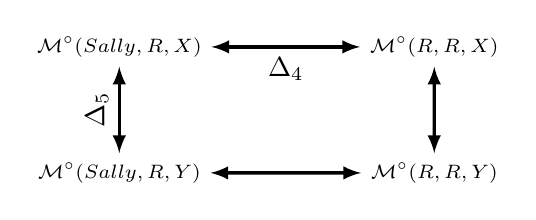
\begin{tikzpicture}[>=latex, scale=0.4]

            \draw(0,0) node (a) {\scriptsize \Model{Sally}{R}{ X}};
            \draw(10,0) node (b) {\scriptsize \Model{R}{R}{ X}};
            \draw(10,-4) node (c) {\scriptsize \Model{R}{R}{ Y}};
            \draw(0,-4) node (d) {\scriptsize \Model{Sally}{R}{ Y}};
            \draw[<->,very thick] (a) -- (b) node[midway, below] {$\Delta_4$};
            \draw[<->,very thick] (b) -- (c);
            \draw[<->,very thick] (c) -- (d);
            \draw[<->,very thick] (d) -- (a) node[midway, sloped, above] {$\Delta_5$};

        \end{tikzpicture}
    \end{multicols}



\end{frame}

%%%%%%%%%%%%%%%%%%%%%%%%%%%%%%%%%%%%%%%%%%%%%%%%%%%%%%%%

\imageframe[caption="Theory of Mind tasks"]{zoo}

%%%%%%%%%%%%%%%%%%%%%%%%%%%%%%%%%%%%%%%%%%%%%%%%%%%%%%%%

{ \paper{Wimmer and Perner, {\bf Beliefs about beliefs: Representation and
constraining function [...]}, Cognition, 1983]\newline
        [Lemaignan, Dillenbourg {\bf Mutual Modelling in Robotics: Inspirations for the Next Steps} -- HRI 2015}

\begin{frame}{1st order ToM: the False-Belief Experiment}

        \begin{center} \includegraphics[width=0.7\textwidth]{sally_ann.pdf}
        \end{center} \end{frame} }

%%%%%%%%%%%%%%%%%%%%%%%%%%%%%%%%%%%%%%%%%%%%%%%%%%%%%%%%

{
\paper{Dillenbourg, Lemaignan et al., {\bf The Symmetry of Partner Modelling}, Intl. J. of Computer Supported Collaborative Learning 2016}
\begin{frame}{The False-Belief Experiment, reloaded}
    \centering
    \only<1>{
        \includegraphics[width=0.7\textwidth]{triadic_false_beliefs.pdf}

    }

    \only<2>{
        \begin{multicols}{2}

            \includegraphics[width=0.9\columnwidth]{triadic_false_beliefs.pdf}

            \columnbreak

            \mbox{}\vfill

            \begin{itemize}
                \item \model{A}{B}{X}
                \item \Model{A}{B}{X}
            \end{itemize}

            \scriptsize
            e.g. {\color{hriSec1} \model{\text{robot}}{\text{Sally}}{plans}}

            \vfill\mbox{}

        \end{multicols}
    }

    \only<3>{
        \begin{itemize}
            \item {\bf Robot is the observer}\\
                \Model{R}{\text{Sally}|\text{Ann}}{plans}? can the human
                verbalise it? i.e. \model{H}{R}{\Mmodel{R}{H}{plans}}?

            \item {\bf Robot is an active participant}\\
                \model{H}{R}{knowledge|plans|goals}? i.e. How Ann interprets the
                behaviour of a robot who moves the ball from the beige box to
                the blue box while Sally is away?

        \end{itemize}
    }
    \only<4>{
        \begin{multicols}{2}
            \vspace*{0.4cm}
            \includegraphics[width=0.9\columnwidth]{triadic_false_beliefs.pdf}



            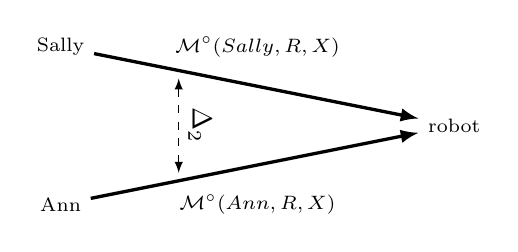
\begin{tikzpicture}[
                    >=latex,
                scale=0.5]

                \draw(0,2) node (A) {\scriptsize Sally};
                \draw(0,-2) node (B) {\scriptsize Ann};
                \draw(10,0) node (C) {\scriptsize robot};

                \draw(5,2) node {\scriptsize \Model{Sally}{ R}{ X}};
                \draw(5,-2) node {\scriptsize \Model{Ann}{ R}{ X}};
                \draw[dashed, <->] (3,1.2) -- (3,-1.2) node[midway, sloped, above] {$\Delta_2$};
                \draw[->,very thick] (A) to (C);
                \draw[->,very thick] (B) to (C);

            \end{tikzpicture}

            \vspace*{1cm}

            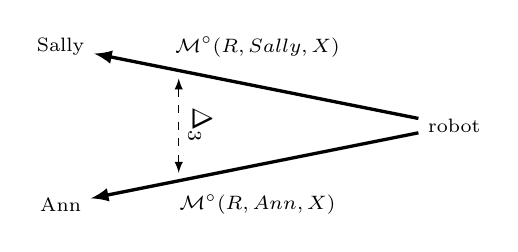
\begin{tikzpicture}[
                    >=latex,
                scale=0.5]

                \draw(0,2) node (A) {\scriptsize Sally};
                \draw(0,-2) node (B) {\scriptsize Ann};
                \draw(10,0) node (C) {\scriptsize robot};

                \draw(5,2) node {\scriptsize \Model{R}{ Sally}{ X}};
                \draw(5,-2) node {\scriptsize \Model{R}{ Ann}{ X}};
                \draw[dashed, <->] (3,1.2) -- (3,-1.2) node[midway, sloped, above]
                {$\Delta_3$};
                \draw[<-,very thick] (A) to (C);
                \draw[<-,very thick] (B) to (C);

            \end{tikzpicture}
        \end{multicols}
    }
    \only<5>{
        Do Sally and Ann have the same accuracy when modelling the robot?

        {\centering
            \(\Delta_2 = \Delta(\Mmodel{\text{Sally}}{R}{X}, \Mmodel{\text{Ann}}{R}{X})\)

        }

        \vspace*{1em}
        Conversely, what may lead the robot to model more accurately
        Sally or Ann?

        {\centering
            \(\Delta_3= \Delta(\Mmodel{R}{\text{Sally}}{X}, \Mmodel{R}{\text{Ann}}{X})\)

        }

    }
\badge{europe_epfl}
\end{frame}
}

%%%%%%%%%%%%%%%%%%%%%%%%%%%%%%%%%%%%%%%%%%%%%%%%%%%%%%%%

{
    \paper{Flobbe et al. {\bf Children's application of theory of mind in
    reasoning and language}, J. of Logic, Language and Information, 2008]\newline
           [Lemaignan, Dillenbourg {\bf Mutual Modelling in Robotics: Inspirations for the Next Steps} -- HRI 2015}
    \begin{frame}{2nd order ToM: the Chocolate Bar Experiment}
        \begin{center}
            \includegraphics[width=0.65\textwidth]{tom/chocolate-bar.pdf}
        \end{center}

    \end{frame}
}

%%%%%%%%%%%%%%%%%%%%%%%%%%%%%%%%%%%%%%%%%%%%%%%%%%%%%%%%

{
    \paper{Verbrugge, {\bf Logic and social cognition}, Journal of Philosophical
    Logic, 2009]\newline
           [Lemaignan, Dillenbourg {\bf Mutual Modelling in Robotics: Inspirations for the Next Steps} -- HRI 2015}
\begin{frame}{Agreement as $\infty$-order ToM}
    \only<1>{
        \begin{center}
            \includegraphics[width=0.4\textwidth]{mutual-agreement.pdf}
        \end{center}
    }
    \only<2->{
        \begin{center}
            \includegraphics[width=0.2\textwidth]{mutual-agreement.pdf}
        \end{center}

    \uncover<2->{
        Shared knowledge
    \[
        \mathsf{EK}_J\varphi \leftrightarrow \bigwedge_{i \in J}\mathsf{K}_i\varphi
    \]
}
    \uncover<3>{
        Common knowledge 
    \[
        \mathsf{CK}_J\varphi \leftrightarrow
    \mathsf{EK}_J\varphi \wedge \mathsf{EK}_J\mathsf{EK}_J\varphi \wedge
    \mathsf{EK}_J\mathsf{EK}_J\mathsf{EK}_J\varphi \wedge ...
    \]
}
}
\end{frame}
}

%%%%%%%%%%%%%%%%%%%%%%%%%%%%%%%%%%%%%%%%%%%%%%%%%%%%%%%%

{
    \paper{Frith and Happé {\bf Autism: Beyond "theory of mind"} -- Cognition, 1994]\newline
           [Lemaignan, Dillenbourg {\bf Mutual Modelling in Robotics: Inspirations for the Next Steps} -- HRI 2015}
\begin{frame}{Shopping list for HRI?}
    \centering
    \begin{tabular}{p{0.45\linewidth}p{0.45\linewidth}}
        \toprule
        {\bf Already in the HRI fridge} & {\bf To buy...} \\
        \midrule
        Instrumental gestures & Expressive gestures \\
        Using person as tool & Using person as receiver of information \\
        Talking about desires and emotions & Talking about beliefs and ideas \\
        Showing "active" sociability & Showing "interactive" sociability \\
        Elicited structured play & Spontaneous pretend play \\
        \bottomrule
    \end{tabular}
        \badge{europe_epfl}
\end{frame}
}

%%%%%%%%%%%%%%%%%%%%%%%%%%%%%%%%%%%%%%%%%%%%%%%%%%%%%%%%

{
    \paper{Frith and Happé {\bf Autism: Beyond "theory of mind"} -- Cognition, 1994]\newline
           [Lemaignan, Dillenbourg {\bf Mutual Modelling in Robotics: Inspirations for the Next Steps} -- HRI 2015}
\begin{frame}{Autistic assets and deficits observed in real life}
    \centering
    \begin{tabular}{p{0.45\linewidth}p{0.45\linewidth}}
        \toprule
        {\bf Assets} & {\bf Deficits} \\
        \midrule
        Instrumental gestures & Expressive gestures \\
        Using person as tool & Using person as receiver of information \\
        Talking about desires and emotions & Talking about beliefs and ideas \\
        Showing "active" sociability & Showing "interactive" sociability \\
        Elicited structured play & Spontaneous pretend play \\
        \bottomrule
    \end{tabular}
        \badge{europe_epfl}
\end{frame}
}

%%%%%%%%%%%%%%%%%%%%%%%%%%%%%%%%%%%%%%%%%%%%%%%%%%%%%%%%

\section{Dynamics of Interaction}

%%%%%%%%%%%%%%%%%%%%%%%%%%%%%%%%%%%%%%%%%%%%%%%%%%%%%%%%

{
\paper{Lemaignan, Fink, Dillenbourg, Braboszcz {\bf The Cognitive Correlates of Anthropomorphism}, HRI 2014}
\begin{frame}[label=anthropomorphism]{How do we perceive robot over time?}
    \begin{figure}
        \centering
        \resizebox{0.8\paperwidth}{!}{

            \begin{tikzpicture}

                % background shading
                \path[fill=hriSec2!50] (0,0) rectangle (0.6,5.5);
                \path[fill=hriSec1Comp!50] (0.6,0) rectangle (5.2,5.5);
                \path[fill=hriSec3Comp!50] (5.2,0) rectangle (9.8,5.5);
                \draw(0.5,5.5) node[anchor=south west, rotate=10] {\scriptsize \sc Initialization};
                \draw(3,5.5) node[anchor=south west, rotate=10] {\scriptsize \sc Familiarization};
                \draw(6.5,5.5) node[anchor=south west, rotate=10] {\scriptsize \sc Stabilization};
                % horizontal axis
                \draw[->] (0,0) -- (10,0) node[anchor=north] {$t$};
                \draw(5,-0.1) node[anchor=north] {\scriptsize Interaction history};


                % vertical axis
                \draw[->] (0,0) -- (0,6) node[anchor=east] {};
                \draw(-0.8,3) node[rotate=90,anchor=south] {\scriptsize Anthropomorphic effects};

                \draw (-0.05, 2.1) -- (0.05, 2.1) node[anchor=east] {\IPA};
                \draw (-0.05, 5) -- (0.05, 5) node[anchor=east] {\AntMax};

                % vertical axis - end
                \draw[->] (9.8,0) -- (9.8,4) node[anchor=east] {};
                \draw (9.8, 0.8) node[anchor=west] {\SLA};


                \draw[<-] (1.15,5.1) -- (1.30,5.3) node[anchor=east] {};
                \draw (1.35,5.4) node[anchor=west] {\tiny \it novelty peak};

                \draw[dashed] (1.1, 0) -- (1.1,5.1);
                \draw (1.1,0) node[anchor=north] {$t_{max}$};

                %\draw[dotted] (0, 5) -- (6.2,5);
                %\draw[dotted] (0, 3) -- (6.2,3);
                %\draw[<->] (6.1,3) -- (6.1,5) node[sloped, above, midway] {$\Delta_{a}$};

                \draw[<-] (2.2,4.4) -- (3.7,4.1) node[anchor=east] {};
                \draw[<-] (3.3,2.6) -- (3.7,4.1) node[anchor=east] {};
                \draw (3.8,4.1) node[anchor=west, align=center] {\tiny \it disruptive\\ \tiny
                \it behaviors};
                %%%%%
                %% CURVES
                %%%%
                \begin{scope}[yscale=-1,shift={(-0.125,-0.46)}]
                    \draw[ultra thick, green!70!red!50, dashed] svg[scale=1cm] "M 0.114,-1.1 C 0.733,-2.79 1.88,-2.23
                    2.51,-1.76 3.34,-1.14 3.94,0.02 10.1,0";

                    \draw[ultra thick, blue!70!red!50, dashed] svg[scale=1cm] "M 0.125,-3.21 C 0.549,-4.91 2.05,-4.42
                    2.59,-3.83 3.57,-2.74 5.93,-1.51 10.1,-1.53";

                    \draw[ultra thick, red!70, dashed] svg[scale=1cm] "M 0.12500001,-2.7222489 C 0.70533638,-5.3401235 1.9431386,-3.7307246 2.608741,-3.3299187 c 1.3619528,0.8201274 3.3166657,1.2251393 7.515191,1.2014756";

                    \draw[ultra thick] svg[scale=1cm] "M
                    0.125,-1.622832 c 0.19887378,-2.35086 0.74751962,-2.9373641 1.0765913,-2.9404859 0.3290717,-0.00312 0.5370891,0.383599 0.754419,0.6452353 0.069872,0.099803 0.1021612,-0.2231749 0.1792538,-0.2238964 0.099707,0 0.013454,0.4985362 0.3173383,0.9139831 0.1911917,0.2612926 0.3444354,0.2578391 0.6711932,0.4894291 0.2058265,0.1458798 0.1571532,0.9762306 0.2615031,0.9702183 0.097182,0 0.083295,-0.3336208 0.4330446,-0.1199242 0.4306401,0.2631203 0.216699,0.1355642 0.4296663,0.2647074 2.0858202,1.13836043 3.8496455,1.41300027 5.8769904,1.43753027";



                \end{scope}

            \end{tikzpicture}
        }
    \end{figure}

        \badge{europe_epfl}
        \backbutton{}
\end{frame}
}

%%%%%%%%%%%%%%%%%%%%%%%%%%%%%%%%%%%%%%%%%%%%%%%%%%%%%%%%

{
\paper{Lemaignan, Fink, Dillenbourg, Braboszcz {\bf The Cognitive Correlates of Anthropomorphism}, HRI 2014}
\begin{frame}{Cognitive Interpretation?}

    \begin{figure}
        \centering
        \resizebox{0.9\paperwidth}{!}{
            \begin{tikzpicture}
                \baselineskip=8pt

                \path[fill=hriSec1Comp!50] (0,0) rectangle (10.5,2);
                \path[fill=hriSec1!50] (0,2) rectangle (10.5,4);
                \path[fill=hriSec3Comp!50] (0,4) rectangle (10.5,6);

                \draw (-0.3,1) node[rotate=90] {Stage 1}
                (-0.3,3) node[rotate=90] {Stage 2}
                (-0.3,5) node[rotate=90] {Stage 3};

                \draw[->] (0,0) -- (11,0) node[anchor=north] {$t$};
                \draw[-|] (0,0) -- (0,6.5) node[anchor=east] {};
                % Us
                \draw[ultra thick, ->] (0,0) -- (1,2) -- (3,2) -- (4,4) -- (6,4) -- (7,6) --
                (9.5,6);
                \draw[ultra thick, dashed, ->] (3,2) -- (9.5,2);
                \draw[ultra thick, dashed, ->] (6,4) -- (9.5,4);

                \draw (11,1) node[align=left, anchor=west]{\scriptsize pre-cognitive\\\scriptsize anthropomorphism}; %label

                \draw (11,3) node[align=left, anchor=west] {\scriptsize{projection of existing}\\\scriptsize{mental models}\\\scriptsize{\it (familiarity)}}; %label

                \draw (11,5) node[align=left, anchor=west] {\scriptsize{adapted mental
                model} \\ $\to$ \scriptsize{adapted interaction}\\\scriptsize{\it (anthropomorphic or not)}}; %label


                \draw[dashed,->] (1,0.1) to[bend right] (2,1.9)  node at (4.5,1) {\tiny{\it observation (shape, motion, sound)}}; %label

                \draw[dashed,->] (4,2.1) to[bend right] (5,3.9)  node[align=left] at (7.5,3) {\tiny \it observation (interactive behavior) \\ \tiny \it or short interaction}; %label

                \draw[dashed,->] (7,4.1) to[bend right] (8,5.9)  node[align=left] at (9,5)
                {\tiny \it contextualized\\ \tiny \it interaction}; %label

            \end{tikzpicture}
        }
    \end{figure}

        \badge{europe_epfl}
\end{frame}
}

%%%%%%%%%%%%%%%%%%%%%%%%%%%%%%%%%%%%%%%%%%%%%%%%%%%%%%%%

\begin{frame}{Unexpected behaviours}

    \centering
    \begin{tabular}{  >{\centering\arraybackslash}m{2cm} | >{\centering\arraybackslash}m{2cm} | >{\centering\arraybackslash}m{2cm} }
        & Unplanned by the robot & Planned by the robot \\ \hline
        Perceived as non-intentional & A  & B  \\ \hline
        Perceived as intentional &  C & D 
    \end{tabular}

    \video{0.4\paperwidth}{videos/ranger-correct.m4v}
    \video{0.4\paperwidth}{videos/ranger-disobey.m4v}

\badge{europe_epfl}
\end{frame}

%%%%%%%%%%%%%%%%%%%%%%%%%%%%%%%%%%%%%%%%%%%%%%%%%%%%%%%%

\begin{frame}{Cognitive Context and Anthropomorphism}
    \begin{center}
        \includegraphics[width=0.45\linewidth]{stimulus-toys}
        \hspace*{1cm}
        \includegraphics[width=0.45\linewidth]{cognitive-priming}
    \end{center}
        \badge{europe_epfl}
\end{frame}

%%%%%%%%%%%%%%%%%%%%%%%%%%%%%%%%%%%%%%%%%%%%%%%%%%%%%%%%

\section{Cognitive Architectures}

%%%%%%%%%%%%%%%%%%%%%%%%%%%%%%%%%%%%%%%%%%%%%%%%%%%%%%%%

{
\paper{Baxter, Lemaignan, Trafton {\bf Workshop on Cognitive Architectures for Social HRI} -- HRI 2016}
\begin{frame}{Cognitive Architectures for social HRI}

    \begin{multicols}{2}
        \resizebox{0.7\columnwidth}{!}{%
            \begin{tikzpicture}[
                    >=latex,
                every edge/.style={<-, draw, very thick}]

            \path[small mindmap, 
                level 1 concept/.append style={sibling angle=360/6}, 
                level 2 concept/.append style={sibling angle=60}, 
            concept color=hriSec1,text=white]
            node[concept] {Cognitive Architectures}
                [clockwise from=60]
                child[concept color=hriSec3Dark,text=white] { node[concept]{1. Model} }
                child[concept color=hriSec2Dark,text=white] { node[concept]{2. Integration} }
                child[concept color=hriSec2CompDark,text=white] { node[concept] {3. Methodology}};


        \end{tikzpicture}
    }
    \vfill
    \columnbreak

    {\bf 1. Models of Human Cognition}

    {\scriptsize -- Modelling (aspects of) human cognition \\-- Subsequent application to robots}

    {\bf 2. Technical Integration}

    {\scriptsize -- Define required functionality of robots \\-- Implement algorithms (etc) necessary}

    {\bf 3. A Methodology}

    {\scriptsize -- Formalising assumptions \\-- Integrating knowledge from multiple disciplines \\-- Iteratively updating architecture}

    %\refToContrib{Someone here...}

    \end{multicols}
        \badge{europe_plym}
\end{frame}
}

%%%%%%%%%%%%%%%%%%%%%%%%%%%%%%%%%%%%%%%%%%%%%%%%%%%%%%%%

{

    \paper{Devin et al. {\bf Some essential skills and their combination in an architecture for a cognitive and interactive robot} -- HRI 2016}
\begin{frame}{``Modeling of human cognition''...}

\resizebox{!}{0.7\paperheight}{%
\tikzset{subpart/.style={draw, font=\scriptsize, fill opacity=0.5, text opacity=1, fill=white!50}}
\begin{tikzpicture}[
    >=latex,
    node distance=1.5,
    every edge/.style={draw, very thick},
    skill/.style={draw, rounded corners, align=center, inner sep=5pt, fill=black!20},
    stmt/.style={align=center, font=\bf},
    label/.style={midway, align=center, font=\scriptsize, fill=white}]

    \node at (0,0)[skill, fill=hriSec2!50] (a1) {Shared Plan Elaboration};

    \node [skill, fill=hriSec2!50,above=of a1] (a2) {Intention Prediction};
    \node [skill, fill=hriSec2!50,left=of a1] (a3) {Mental State Management};
    \node [skill, fill=hriSec2!50,right=of a1] (a4) {Communication for\\Joint Action};
    \node [skill, fill=hriSec2!50,below=of a1] (a5) {Shared Plan Achievement};
    \node [skill, fill=hriSec2!50,left=of a5] (a6) {Situation Assessment};


    \node [skill, fill=hriSec3!50,below left=of a5,anchor=north] (a7) {Action Achievement};
    \node [skill, fill=hriSec3!50,below right=of a5,anchor=north] (a8) {Human Action Monitoring};
  
    \node[below=3.7 of a5] (a14) {Human-aware geometric and task planners, real-time controllers, sensors...};

  \coordinate[below=3 of a6] (a9);

  \node[rotate=90,left=0.7 of a3.west] (distal) {\bf\large DISTAL};
  \node[rotate=90] at (distal |- a7.south) {\bf\large PROXIMAL};
  \node[rotate=90] at (distal |- a14) {\bf\large MOTOR};

  \coordinate (a11) at (a9 -| distal.north);
  \coordinate (a12) at (a9 -| a4.east);
  \draw[dotted, thick] (a11) -- (a12);


  \coordinate (a13) at ($(a5)!0.5!(a7)$);
  \draw[dotted, thick] (a13 -| distal.north) -- (a13 -| a4.east);


  %%% Relations between components
  \path (a2) edge [->] node[label] {goal to execute} (a1);
  \path (a1) edge [->] node[label] {plan} (a5);
  \path (a2) edge [<-] node[label] {goal (order)} (a4);

  \path (a3) edge [<->, bend left=40, looseness=1.2] node[label,pos=0.1] {mental state information} (a4);
  \path (a3) edge [<->] (a2);
  \path (a3) edge [<->] (a1);
  \path (a3) edge [<->] (a5);

  \path (a6) edge [->] node[label] {conceptual\\world state} (a3);

  \path (a5) edge [<->] node[label] {coordination} (a4);

  \path (a5) edge [<->] node[label,right=0.5] {anchoring of actions} (a7);
  \path (a5) edge [<->] (a8);

  \path (a9) edge [->] node[label] {sensors} (a6);

  \coordinate (a10) at (a9 -| a7);
  \path (a10) edge [<->] node[label] {planning and control} (a7);

  \coordinate (a10) at (a9 -| a8);
  \path (a10) edge [<->] node[label] {sensors} (a8);

  \path (a7) edge [<->] node[label] {coordination} (a8);
 
\end{tikzpicture}
}

\end{frame}
}

%%%%%%%%%%%%%%%%%%%%%%%%%%%%%%%%%%%%%%%%%%%%%%%%%%%%%%%%
%%%%%%%%%%%%%%%%%%%%%%%%%%%%%%%%%%%%%%%%%%%%%%%%%%%%%%%%

%%%%%%%%%%%%%%%%%%%%%%%%%%%%%%%%%%%%%%%%%%%%%%%%%%%%%%%%
%%%%%%%%%%%%%%%%%%%%%%%%%%%%%%%%%%%%%%%%%%%%%%%%%%%%%%%%
%%%%%%%%%%%%%%%%%%%%%%%%%%%%%%%%%%%%%%%%%%%%%%%%%%%%%%%%




\end{document}
